% !TeX program = xelatex
% !TeX encoding = UTF-8
% Presentazione revisionata: Basalto · Dal codice al calcolo scientifico
% Basata sul materiale originale fornito dall'autore e sul template M01_Pensare_con_i_dati.tex
% Compilazione: xelatex -interaction=nonstopmode T00_Basalto.tex (due passaggi)
% Diagrammi TikZ e figure statistiche vettoriali; sorgenti R e dati inclusi.
% 66 slide. Materiali del corso e impaginazione della serie planetaria.
\RequirePackage{fix-cm}
\documentclass[12pt,aspectratio=1610]{beamer}
\geometry{paperwidth=20cm,paperheight=12.5cm}
\usepackage[italian,provide=*]{babel}
\usepackage{fontspec,adjustbox,tabularx}
\IfFontExistsTF{NimbusSans-Regular.otf}{
\setsansfont{NimbusSans-Regular.otf}[BoldFont=NimbusSans-Bold.otf,ItalicFont=NimbusSans-Italic.otf,BoldItalicFont=NimbusSans-BoldItalic.otf]
\setmainfont{NimbusSans-Regular.otf}[BoldFont=NimbusSans-Bold.otf,ItalicFont=NimbusSans-Italic.otf,BoldItalicFont=NimbusSans-BoldItalic.otf]
}{
\setsansfont{TeX Gyre Heros}
\setmainfont{TeX Gyre Heros}
}
\IfFontExistsTF{DejaVu Sans Mono}{
\setmonofont{DejaVu Sans Mono}[Scale=.88]
}{\setmonofont{Latin Modern Mono}[Scale=.88]}
\usefonttheme{professionalfonts}
\usepackage{amsmath,amssymb,booktabs,array,graphicx,tikz,bookmark}
\usetikzlibrary{calc,positioning,arrows.meta}
\graphicspath{{Figure/}}
\definecolor{Paper}{HTML}{F8F6F1}
\definecolor{Ink}{HTML}{253344}
\definecolor{Navy}{HTML}{15283E}
\definecolor{Quantum}{HTML}{5146A5}
\definecolor{Classical}{HTML}{087C74}
\definecolor{Muted}{HTML}{657180}
\definecolor{Rule}{HTML}{D6DAD9}
\definecolor{Night}{HTML}{112236}
\definecolor{Lilac}{HTML}{ABB5FF}
\definecolor{Mint}{HTML}{72D8C8}
\setbeamercolor{background canvas}{bg=Paper}
\setbeamercolor{normal text}{fg=Ink}
\setbeamertemplate{navigation symbols}{}
\setbeamertemplate{headline}{}
\setbeamertemplate{footline}{}
\setbeamersize{text margin left=0pt,text margin right=0pt}
\hypersetup{colorlinks=true,linkcolor=Classical,urlcolor=Classical,pdfpagemode=UseOutlines,pdfstartview=Fit,
 pdftitle={Basalto · Dal codice al calcolo scientifico},pdfauthor={GeoStat Lab · materiali di Marzio De Corato},
 pdfsubject={GeoStat Lab · T00}}
\bookmarksetup{open,openlevel=0,depth=2}
\newsavebox{\BodyBox}
\newsavebox{\SideBox}
\newsavebox{\RecallBox}
\newsavebox{\TitleBox}
\newcommand{\MeasureBox}[2]{\typeout{REVIEWBOX:#1:\the\wd#2:\the\ht#2:\the\dp#2}}

% Revisione completa: diagrammi TikZ, formalismo e box R.
\usepackage[most]{tcolorbox}
\usepackage{listings}
\usetikzlibrary{fit,backgrounds,matrix,decorations.pathreplacing}
\definecolor{GeoA}{HTML}{1D7890}
\definecolor{GeoB}{HTML}{C57E42}
\definecolor{GeoC}{HTML}{7363AA}
\definecolor{GeoTint}{HTML}{F0F4F3}
\lstdefinestyle{GeoR}{language=R,basicstyle=\ttfamily\fontsize{9.2}{12.2}\selectfont,
 keywordstyle=\color{Quantum}\bfseries,commentstyle=\color{Classical},stringstyle=\color{GeoB},
 numbers=left,numberstyle=\tiny\color{Muted},numbersep=4pt,showstringspaces=false,
 columns=fullflexible,keepspaces=true,breaklines=true,xleftmargin=1.15em,
 frame=none,aboveskip=0pt,belowskip=0pt,tabsize=2}
\newsavebox{\PilotLeftBox}
\newsavebox{\PilotRightBox}
\newcommand{\PLabel}[1]{\par{\color{Classical}\bfseries\fontsize{9}{11}\selectfont\MakeUppercase{#1}}\par\vspace{1.8mm}}
\newcommand{\PBody}[1]{\par{\fontsize{11.3}{14.8}\selectfont #1\par}}
\newcommand{\PSmall}[1]{\par{\fontsize{9.8}{13.1}\selectfont #1\par}}
\newcommand{\PCode}[2]{%
\begin{tcolorbox}[enhanced,arc=1.8mm,boxrule=.65pt,
  colback=white,colframe=Classical!75!Navy,colbacktitle=Navy,
  coltitle=white,fonttitle=\bfseries\fontsize{9.6}{12}\selectfont,
  title={#1},left=1.7mm,right=1.3mm,top=1.5mm,bottom=1.3mm,
  before skip=1mm,after skip=1mm]
\lstinputlisting[style=GeoR]{Codice/#2}
\end{tcolorbox}}
\newcommand{\PInfo}[1]{%
\begin{tcolorbox}[enhanced,arc=1.6mm,boxrule=.55pt,colback=GeoTint,
 colframe=Rule!80!Classical,left=2.3mm,right=2.3mm,top=2mm,bottom=2mm,
 before skip=1mm,after skip=1mm]
\PSmall{#1}\end{tcolorbox}}
\tikzset{
 pFlow/.style={draw=Classical!45,fill=white,rounded corners=2mm,
  line width=.7pt,align=center,minimum height=1.1cm,font=\sffamily\fontsize{10}{12}\selectfont},
 pEdge/.style={-{Latex[length=2.3mm]},draw=Classical,line width=.95pt},
 pGroup/.style={draw=Rule,fill=white,rounded corners=2mm,line width=.65pt},
 pDotA/.style={circle,fill=GeoA,inner sep=1.25pt},
 pDotB/.style={circle,fill=GeoB,inner sep=1.25pt},
 pDotC/.style={circle,fill=GeoC,inner sep=1.25pt}
}
\newcommand{\PilotChrome}[4]{%
  \node[anchor=north west,inner sep=0,text width=17.7cm] at ([xshift=.95cm,yshift=-.55cm]current page.north west) {\color{Navy}\bfseries\fontsize{20.6}{24.5}\selectfont #1};
  \node[anchor=north east,inner sep=0] at ([xshift=19.05cm,yshift=-.14cm]current page.north west) {\color{Classical}\fontsize{8}{10}\selectfont\hyperlink{slide2}{#2}};
  \draw[Classical,line width=1.2pt] ([xshift=.95cm,yshift=-1.7cm]current page.north west)--([xshift=2.35cm,yshift=-1.7cm]current page.north west);
  \draw[Rule,line width=.65pt] ([xshift=.95cm,yshift=-10.36cm]current page.north west)--([xshift=19.05cm,yshift=-10.36cm]current page.north west);
  \node[anchor=north west,inner sep=0] at ([xshift=.96cm,yshift=-10.55cm]current page.north west) {\color{Classical}\bfseries\fontsize{9.1}{12}\selectfont DA RICORDARE};
  \node[anchor=north west,inner sep=0,text width=14.3cm] at ([xshift=4.2cm,yshift=-10.53cm]current page.north west) {\color{Ink}\fontsize{10.3}{13.8}\selectfont #4};
  \draw[Rule,line width=.35pt] ([xshift=.95cm,yshift=-11.92cm]current page.north west)--([xshift=19.05cm,yshift=-11.92cm]current page.north west);
  \node[anchor=north west,inner sep=0] at ([xshift=.95cm,yshift=-12.06cm]current page.north west) {\color{Muted}\fontsize{7.7}{9.2}\selectfont Basalto · Dal codice al calcolo scientifico};
  \node[anchor=north east,inner sep=0] at ([xshift=19.05cm,yshift=-12.06cm]current page.north west) {\color{Muted}\fontsize{7.7}{9.2}\selectfont #3/66};
}


% Stili comuni per i diagrammi scientifici della revisione completa.
\tikzset{
 pAxis/.style={-{Latex[length=2mm]},draw=Muted,line width=.65pt},
 pNote/.style={font=\sffamily\fontsize{9}{11.5}\selectfont,text=Muted,align=center},
 pLabel/.style={font=\sffamily\fontsize{10}{12.5}\selectfont,text=Ink,align=center}
}
\newsavebox{\FullWideBox}
\setlength{\emergencystretch}{1em}




\newcommand{\PLab}[2]{\par{\color{Classical}\bfseries\fontsize{9}{11}\selectfont
\href{#1}{\MakeUppercase{#2}}}\par\vspace{1.8mm}}

\definecolor{Measure}{HTML}{A05B10}\definecolor{Rose}{HTML}{9B4564}\definecolor{Wash}{HTML}{EAE7F6}\definecolor{Gold}{HTML}{EEC184}
\tikzset{arr/.style={-{Stealth[length=2mm]},line width=.8pt,draw=Classical}}
\newcommand{\Colonna}[2]{\begin{adjustbox}{max totalsize={#1}{7.95cm},valign=t}\begin{minipage}[t]{#1}\raggedright\fontsize{11.3}{14.8}\selectfont #2\end{minipage}\end{adjustbox}}
\begin{document}



\begin{frame}[plain]\hypertarget{slide1}{}\bookmark[level=0,page=1]{Basalto}
\begin{tikzpicture}[remember picture,overlay]
\fill[Night](current page.south west) rectangle(current page.north east);
\IfFileExists{Scena/copertina.jpg}{\node[inner sep=0] at(current page.center){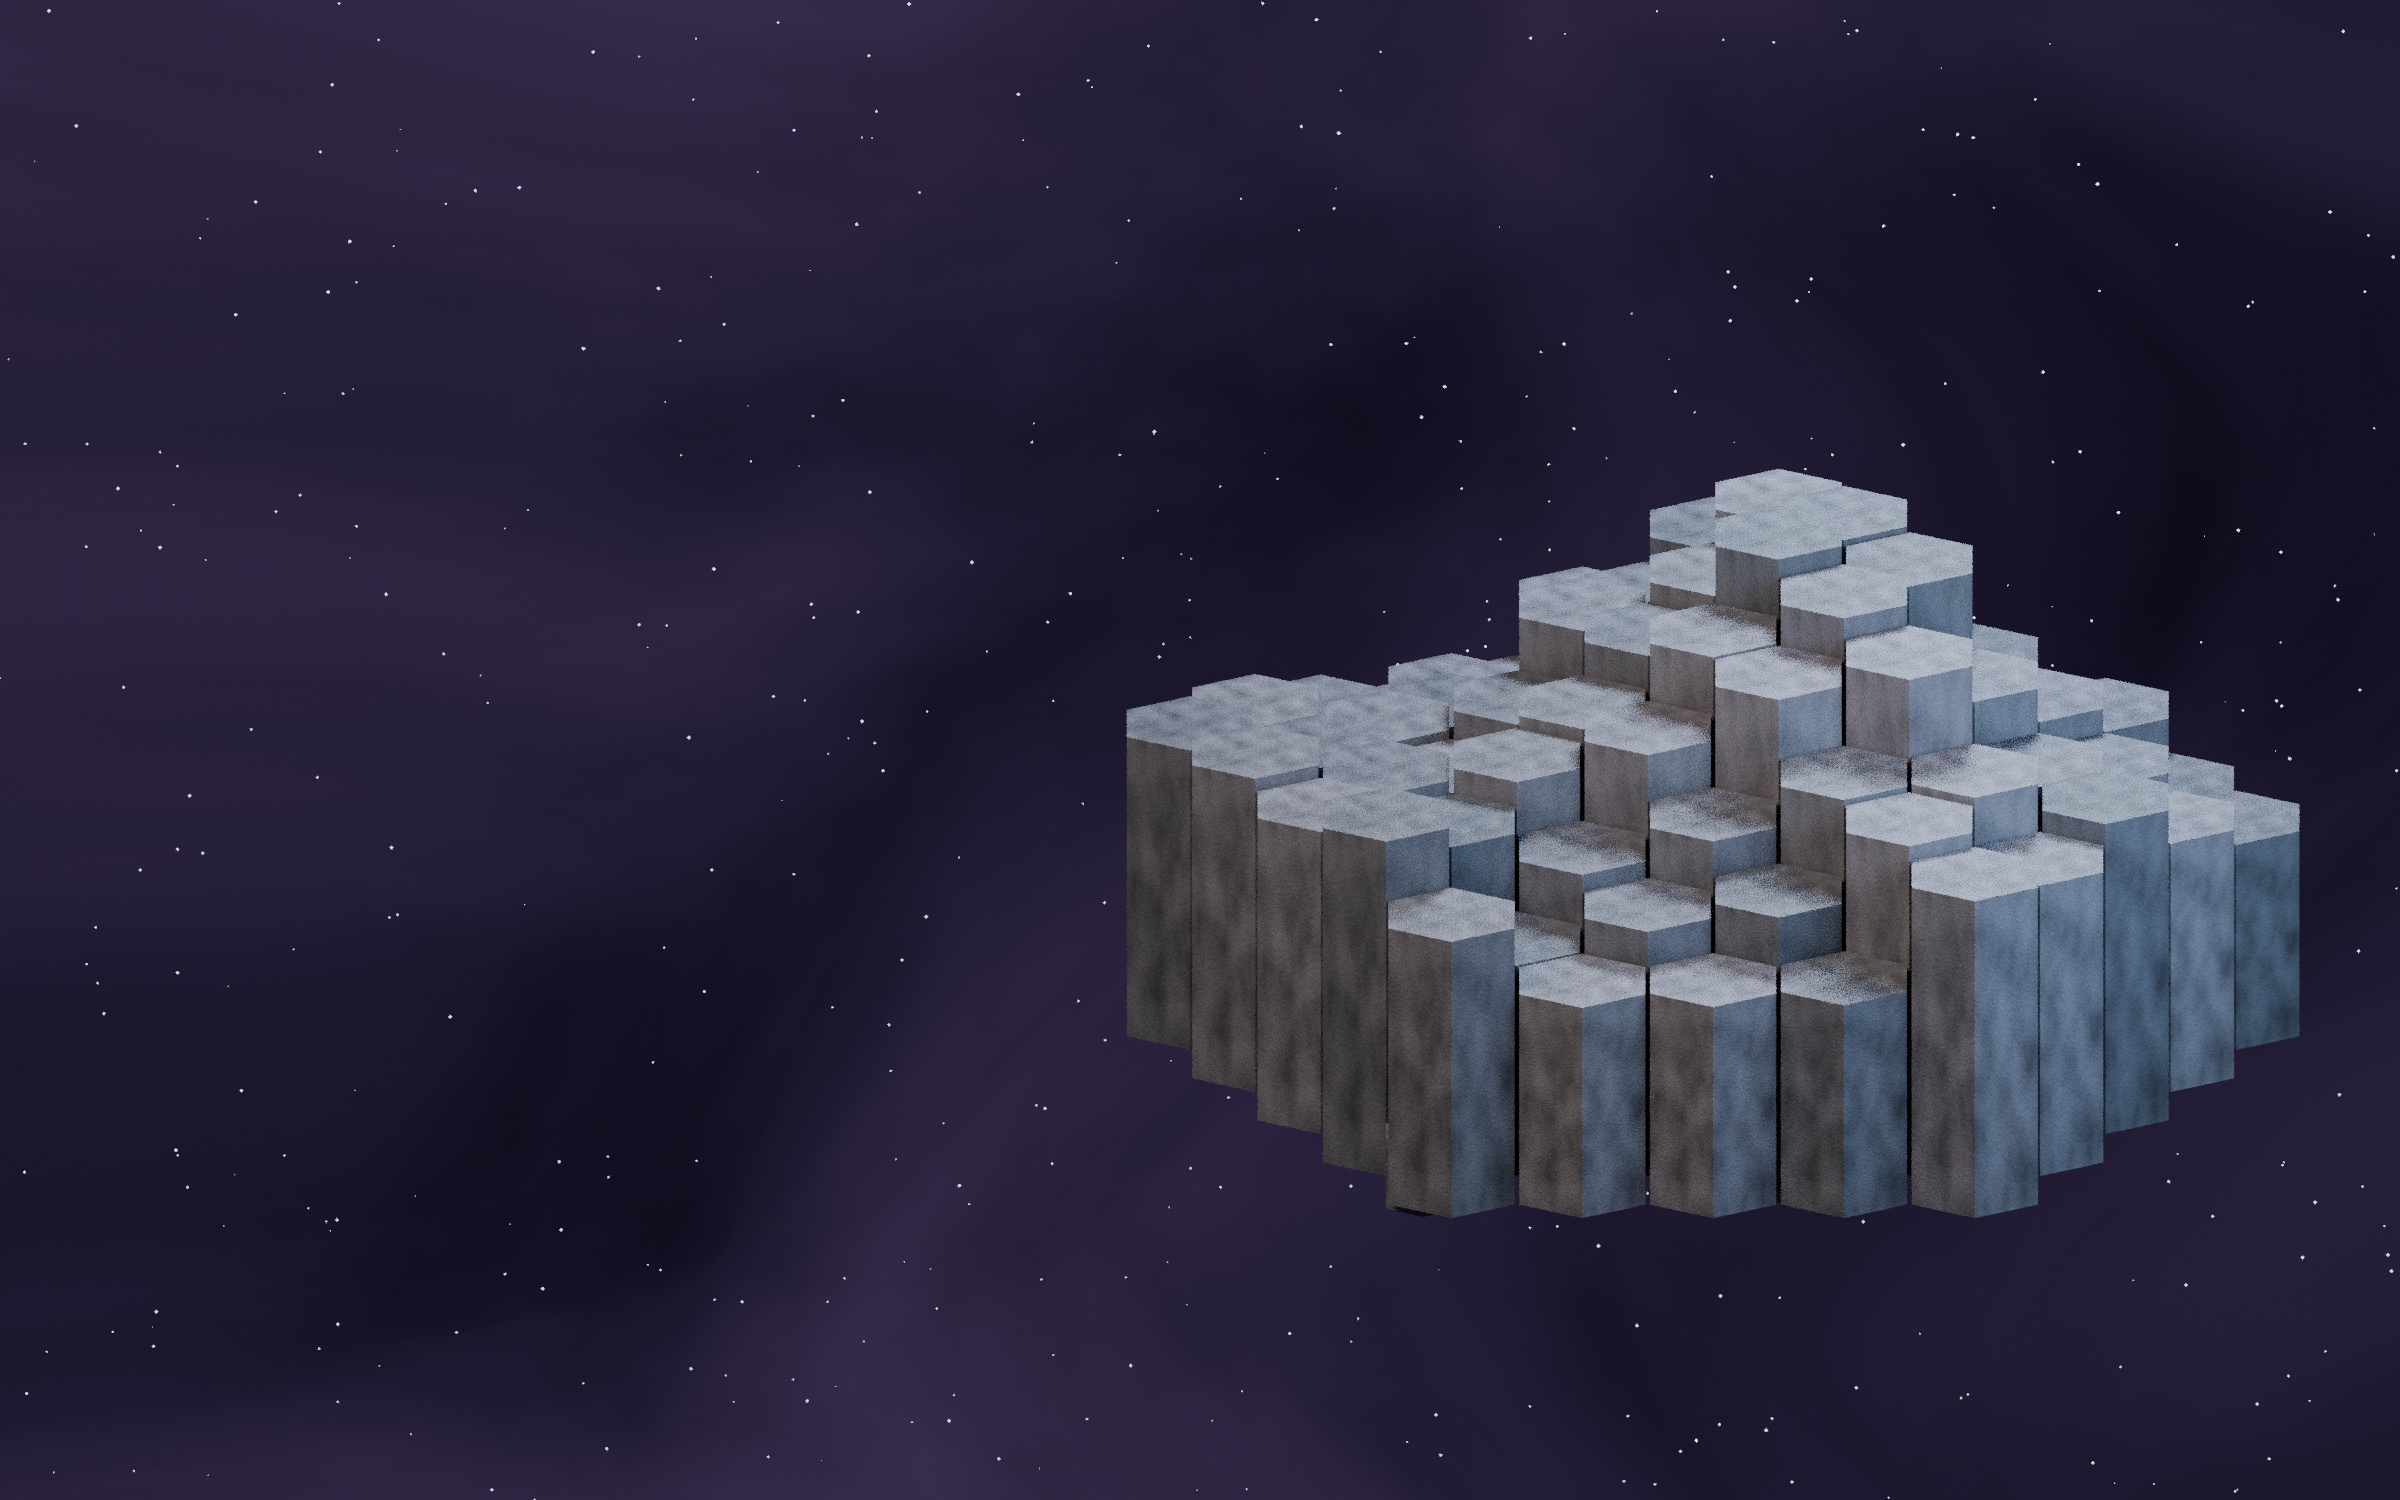
\includegraphics[width=20cm,height=12.5cm]{Scena/copertina.jpg}};}{}
\node[anchor=north west,inner sep=0] at([xshift=1.05cm,yshift=-1.10cm]current page.north west){\color{Mint}\bfseries\fontsize{23}{28}\selectfont BASALTO};
\node[anchor=north west,inner sep=0] at([xshift=1.07cm,yshift=-2.16cm]current page.north west){\color{white}\fontsize{9}{12}\selectfont MODULO T00 · SCIENZE DELLA TERRA};
\draw[Mint,line width=1.5pt]([xshift=1.07cm,yshift=-2.78cm]current page.north west)--([xshift=2.6cm,yshift=-2.78cm]current page.north west);
\node[anchor=north west,inner sep=0] at([xshift=1.05cm,yshift=-3.35cm]current page.north west){\begin{minipage}{9.2cm}\raggedright\color{white}\bfseries\fontsize{28.5}{34.5}\selectfont Dal codice al\\calcolo scientifico\end{minipage}};
\node[anchor=north west,inner sep=0] at([xshift=1.07cm,yshift=-7.88cm]current page.north west){\begin{minipage}{8.9cm}\raggedright\color{Lilac}\fontsize{12.2}{17}\selectfont Un provino, due linguaggi\end{minipage}};
\node[anchor=north west,inner sep=0] at([xshift=1.07cm,yshift=-8.70cm]current page.north west){\begin{minipage}{8.9cm}\raggedright\color{white!75}\fontsize{10.3}{14.5}\selectfont Massa, volume e densità come filo conduttore\end{minipage}};
\node[anchor=north west,inner sep=0] at([xshift=1.07cm,yshift=-10.52cm]current page.north west){\color{white}\fontsize{10.5}{14}\selectfont GeoStat Lab · corso di Marzio De Corato};
\node[anchor=north west,inner sep=0] at([xshift=1.07cm,yshift=-11.17cm]current page.north west){\color{Mint}\fontsize{8.8}{11}\selectfont\href{https://creativecommons.org/licenses/by-nc-sa/4.0/}{Impaginazione da Tessera · CC BY-NC-SA 4.0}};
\end{tikzpicture}\end{frame}
\begin{frame}[plain]\hypertarget{slide2}{}
\bookmark[level=1,page=2]{Indice della presentazione}
\begin{tikzpicture}[remember picture,overlay]
\PilotChrome{Indice della presentazione}{PERCORSO}{2}{I titoli dell’indice aprono i capitoli. Il nome del capitolo in alto riporta a questa pagina.}
\node[anchor=north west,inner sep=0] at([xshift=.96cm,yshift=-2.12cm]current page.north west){\Colonna{9.40cm}{\PLabel{Capitoli}
{\fontsize{10.7}{13.5}\selectfont\hyperlink{slide4}{Dalla domanda al programma\hfill 4}\par}\vspace{.16cm}
{\fontsize{10.7}{13.5}\selectfont\hyperlink{slide12}{Valori, tipi e operazioni\hfill 12}\par}\vspace{.16cm}
{\fontsize{10.7}{13.5}\selectfont\hyperlink{slide20}{Lettura e trasformazione dei dati\hfill 20}\par}\vspace{.16cm}
{\fontsize{10.7}{13.5}\selectfont\hyperlink{slide31}{Errori e controllo del procedimento\hfill 31}\par}\vspace{.16cm}
{\fontsize{10.7}{13.5}\selectfont\hyperlink{slide37}{Preparazione ed esecuzione locale\hfill 37}\par}\vspace{.16cm}
{\fontsize{10.7}{13.5}\selectfont\hyperlink{slide45}{Scelte di strumenti e prestazioni\hfill 45}\par}\vspace{.16cm}
{\fontsize{10.7}{13.5}\selectfont\hyperlink{slide53}{Esecuzione remota e persistenza\hfill 53}\par}\vspace{.16cm}
{\fontsize{10.7}{13.5}\selectfont\hyperlink{slide59}{Confronti e consegna del lavoro\hfill 59}\par}\vspace{.16cm}
}};
\node[anchor=north west,inner sep=0] at([xshift=10.85cm,yshift=-2.12cm]current page.north west){\Colonna{8.16cm}{\PLabel{Percorso di lettura}
\PBody{Il registro contiene 24 provini, quattro per stazione, distribuiti in due affioramenti. Seguiamo dal banco di misura alla tabella la densità del primo provino, C01.}
\PInfo{Le pagine Scenario A e Confronto riprendono gli esperimenti nel browser. I valori di partenza del simulatore possono differire dal caso guida.}
\href{https://marzione00.github.io/Lab_Geo/\#modulo-T00}{\color{Classical}\bfseries Apri gli esperimenti di Basalto}}};
\end{tikzpicture}\end{frame}

\begin{frame}[plain]\hypertarget{slide3}{}
\bookmark[level=1,page=3]{Come si trasforma una misura in un risultato che un’altra persona può ricalcolare?}
\begin{tikzpicture}[remember picture,overlay]
\PilotChrome{{\fontsize{15.3}{19}\selectfont Come si trasforma una misura in un risultato che un’altra persona può ricalcolare?}}{IL CASO GUIDA}{3}{Prima del calcolo annota identificativo, unità e criterio di selezione.}
\node[anchor=north west,inner sep=0] at([xshift=.96cm,yshift=-2.12cm]current page.north west){\Colonna{9.40cm}{{\centering\resizebox{.97\linewidth}{!}{\begin{tikzpicture}[x=1cm,y=1cm]

\foreach \x/\h/\id/\massa/\vol in {0/1.2/C01/{107{,}2}/40,2.8/1.5/C02/{121{,}95}/45,5.6/1.8/C03/{132{,}5}/50}{
 \begin{scope}[shift={(\x,0)}]
 \fill[GeoA!58] (.2,1.4)--(1,1.1)--(1,{1.1+\h})--(.2,{1.4+\h})--cycle;
 \fill[GeoA!83!Navy] (1,1.1)--(1.9,1.5)--(1.9,{1.5+\h})--(1,{1.1+\h})--cycle;
 \fill[GeoA!25] (.2,{1.4+\h})--(1,{1.1+\h})--(1.9,{1.5+\h})--(1.12,{1.82+\h})--cycle;
 \node[font=\bfseries,text=Navy] at (1,.64){\id};
 \node[pNote] at (1,.14){$\massa$ g};
 \node[pNote] at (1,-.35){$\vol$ cm$^3$};
 \end{scope}}
\end{tikzpicture}
}\par}
}};
\node[anchor=north west,inner sep=0] at([xshift=10.85cm,yshift=-2.12cm]current page.north west){\Colonna{8.16cm}{\PLabel{Il caso}
\PBody{Il registro contiene 24 provini, quattro per stazione, distribuiti in due affioramenti. Seguiamo dal banco di misura alla tabella la densità del primo provino, C01.}
\PInfo{Alla fine della lezione saprai verificare in R e Python un rapporto fisico, una selezione di righe e una sintesi di gruppo.}
}};
\end{tikzpicture}\end{frame}

\begin{frame}[plain]\hypertarget{slide4}{}
\bookmark[level=0,page=4]{Dalla domanda al programma}
\bookmark[level=1,page=4]{Tre provini diventano tre densità}
\begin{tikzpicture}[remember picture,overlay]
\PilotChrome{Tre provini diventano tre densità}{DALLA DOMANDA AL PROGRAMMA}{4}{Una densità appartiene allo stesso provino della sua massa e del suo volume.}
\node[anchor=north west,inner sep=0] at([xshift=.96cm,yshift=-2.12cm]current page.north west){\Colonna{9.40cm}{\PLabel{Domanda}
\PBody{Sul banco ci sono i provini C01, C02 e C03. Per ognuno misuriamo massa in grammi e volume in centimetri cubi. Quale operazione conserva l’identità del provino?}
\vspace{.35cm}\PLabel{Interpretazione}
\PBody{Dividendo le colonne riga per riga si ottengono 2,68, 2,71 e 2,65 g/cm³. È possibile risalire da ciascun risultato alla coppia che lo ha prodotto.}
}};
\node[anchor=north west,inner sep=0] at([xshift=10.85cm,yshift=-2.12cm]current page.north west){\Colonna{8.16cm}{\begin{tcolorbox}[enhanced,arc=1.7mm,boxrule=.6pt,colback=white,colframe=Classical!60!Navy,colbacktitle=Navy,coltitle=white,fonttitle=\bfseries\small,title={R · calcolo riproducibile},left=1.7mm,right=1.3mm,top=1.1mm,bottom=1.1mm,before skip=1mm,after skip=1.0mm]\lstinputlisting[style=GeoR,language=R]{Codice/capitolo-01.R}\end{tcolorbox}
\PLabel{Risultato in R}
\begin{tcolorbox}[colback=GeoTint,colframe=Rule,boxrule=.5pt,arc=1.4mm,left=2mm,right=1mm,top=1mm,bottom=1mm]{\fontsize{9}{12}\selectfont\ttfamily \mbox{[1]\ 2.68\ 2.71\ 2.65}}\end{tcolorbox}}};
\end{tikzpicture}\end{frame}

\begin{frame}[plain]\hypertarget{slide5}{}
\bookmark[level=1,page=5]{La stessa operazione in R e Python}
\begin{tikzpicture}[remember picture,overlay]
\PilotChrome{La stessa operazione in R e Python}{DALLA DOMANDA AL PROGRAMMA}{5}{Dividendo le colonne riga per riga si ottengono 2,68, 2,71 e 2,65 g/cm³. È possibile risalire da ciascun risultato alla coppia che lo ha prodotto.}
\node[anchor=north west,inner sep=0] at([xshift=.96cm,yshift=-2.12cm]current page.north west){\Colonna{9.40cm}{\begin{tcolorbox}[enhanced,arc=1.7mm,boxrule=.6pt,colback=white,colframe=Classical!60!Navy,colbacktitle=Navy,coltitle=white,fonttitle=\bfseries\small,title={R},left=1.7mm,right=1.3mm,top=1.1mm,bottom=1.1mm,before skip=1mm,after skip=1.0mm]\lstinputlisting[style=GeoR,language=R]{Codice/capitolo-01.R}\end{tcolorbox}
\PSmall{Caso: Tre provini diventano tre densità.}
}};
\node[anchor=north west,inner sep=0] at([xshift=10.85cm,yshift=-2.12cm]current page.north west){\Colonna{8.16cm}{\begin{tcolorbox}[enhanced,arc=1.7mm,boxrule=.6pt,colback=white,colframe=Classical!60!Navy,colbacktitle=Navy,coltitle=white,fonttitle=\bfseries\small,title={Python 3},left=1.7mm,right=1.3mm,top=1.1mm,bottom=1.1mm,before skip=1mm,after skip=1.0mm]\lstinputlisting[style=GeoR,language=Python]{Codice/capitolo-01.py}\end{tcolorbox}
\PInfo{Una densità appartiene allo stesso provino della sua massa e del suo volume.}
}};
\end{tikzpicture}\end{frame}

\begin{frame}[plain]\hypertarget{slide6}{}
\bookmark[level=1,page=6]{Una domanda geologica diventa una procedura}
\begin{tikzpicture}[remember picture,overlay]
\PilotChrome{Una domanda geologica diventa una procedura}{DALLA DOMANDA AL PROGRAMMA}{6}{Il programma traduce una domanda definita attraverso variabili, unità e operazioni verificabili.}
\node[anchor=north west,inner sep=0] at([xshift=.96cm,yshift=-2.12cm]current page.north west){\Colonna{9.40cm}{{\centering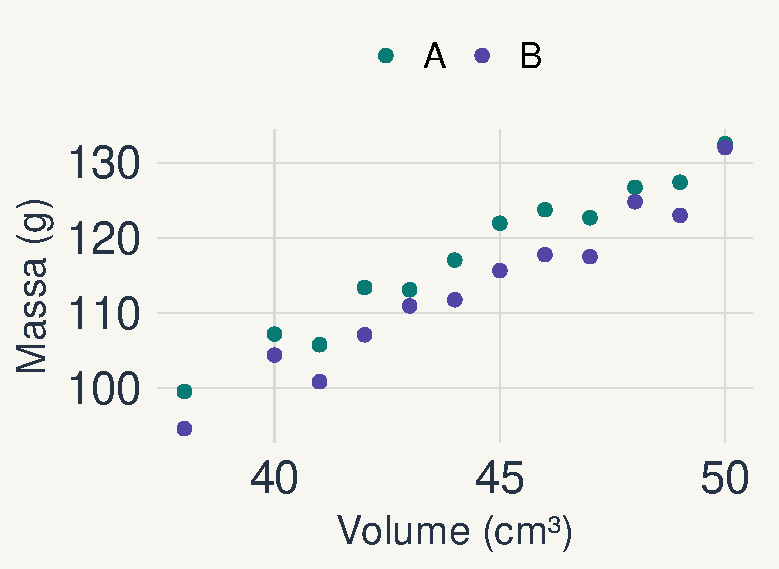
\includegraphics[width=\linewidth,height=6.15cm,keepaspectratio]{Figure/F01.pdf}\par}
\PSmall{Massa e volume dei ventiquattro provini didattici. Il colore identifica l’affioramento di appartenenza.}
}};
\node[anchor=north west,inner sep=0] at([xshift=10.85cm,yshift=-2.12cm]current page.north west){\Colonna{8.16cm}{\PBody{Il corso collega misure, ragionamento statistico e calcolo attraverso procedure delle quali sia possibile ricostruire ogni passaggio. L’introduzione utilizza ventiquattro provini, distribuiti in sei stazioni e due affioramenti, per derivare la densità da massa e volume. Prima di eseguire un comando occorre stabilire il significato delle colonne, le unità e l’oggetto della sintesi. R costituisce il linguaggio principale delle lezioni; gli esercizi Python affiancati permettono di riconoscere quali scelte appartengano al metodo e quali alla sua implementazione.}
}};
\end{tikzpicture}\end{frame}

\begin{frame}[plain]\hypertarget{slide7}{}
\bookmark[level=1,page=7]{Algoritmo, linguaggio e programma}
\begin{tikzpicture}[remember picture,overlay]
\PilotChrome{Algoritmo, linguaggio e programma}{DALLA DOMANDA AL PROGRAMMA}{7}{Il significato della procedura resta distinguibile dagli strumenti con cui viene scritta ed eseguita.}
\node[anchor=north west,inner sep=0] at([xshift=.96cm,yshift=-2.12cm]current page.north west){\Colonna{9.40cm}{{\centering\resizebox{.97\linewidth}{!}{\begin{tikzpicture}[x=1cm,y=-.87cm,every node/.style={font=\fontsize{12.2}{15}\selectfont,text=Ink},arr/.style={-{Stealth[length=2mm]},line width=.8pt,draw=Classical}]\path[use as bounding box] (0,0) rectangle (7.45,6.2);
\draw[draw=Classical,fill=Classical!8,rounded corners=2pt,line width=.7pt] (0.25,0.25) rectangle (7.15,1.6);
\node[anchor=center,text=Classical,font=\fontsize{12}{15}\selectfont,text width=6.5cm,align=center] at (3.7,0.61) {\textbf{Algoritmo}};
\node[anchor=center,text=Ink,font=\fontsize{11.3}{15}\selectfont,text width=6.5cm,align=center] at (3.7,1.2) {Operazioni e dipendenze};
\draw[arr,draw=Classical] (3.7,1.65)--(3.7,1.97);
\draw[draw=Quantum,fill=Quantum!8,rounded corners=2pt,line width=.7pt] (0.25,2.1) rectangle (7.15,3.45);
\node[anchor=center,text=Quantum,font=\fontsize{12}{15}\selectfont,text width=6.5cm,align=center] at (3.7,2.46) {\textbf{Programma}};
\node[anchor=center,text=Ink,font=\fontsize{11.3}{15}\selectfont,text width=6.5cm,align=center] at (3.7,3.05) {Istruzioni nel linguaggio scelto};
\draw[arr,draw=Quantum] (3.7,3.5)--(3.7,3.8200000000000003);
\draw[draw=Classical,fill=Classical!8,rounded corners=2pt,line width=.7pt] (0.25,3.95) rectangle (7.15,5.300000000000001);
\node[anchor=center,text=Classical,font=\fontsize{12}{15}\selectfont,text width=6.5cm,align=center] at (3.7,4.3100000000000005) {\textbf{Runtime}};
\node[anchor=center,text=Ink,font=\fontsize{11.3}{15}\selectfont,text width=6.5cm,align=center] at (3.7,4.9) {Esecuzione delle istruzioni};

\end{tikzpicture}}\par}
}};
\node[anchor=north west,inner sep=0] at([xshift=10.85cm,yshift=-2.12cm]current page.north west){\Colonna{8.16cm}{\PBody{Un algoritmo descrive una sequenza di operazioni, mentre un linguaggio fornisce le regole con cui esprimerla in una forma eseguibile. Un programma è una realizzazione di tale procedura; uno script ne costituisce una forma comunemente conservata in un file di testo. L’ambiente di sviluppo offre strumenti per scrivere, avviare e ispezionare il codice, mentre il runtime ne esegue le istruzioni. Questa distinzione permette di comprendere perché lo stesso file R possa essere utilizzato da un terminale oppure da un’interfaccia come RStudio.}
}};
\end{tikzpicture}\end{frame}

\begin{frame}[plain]\hypertarget{slide8}{}
\bookmark[level=1,page=8]{Interfaccia, processo e sistema di calcolo}
\begin{tikzpicture}[remember picture,overlay]
\PilotChrome{Interfaccia, processo e sistema di calcolo}{DALLA DOMANDA AL PROGRAMMA}{8}{File persistenti e oggetti della sessione occupano ruoli diversi nel procedimento di calcolo.}
\node[anchor=north west,inner sep=0] at([xshift=.96cm,yshift=-2.12cm]current page.north west){\Colonna{9.40cm}{{\centering\resizebox{.97\linewidth}{!}{\begin{tikzpicture}[x=1cm,y=-.87cm,every node/.style={font=\fontsize{12.2}{15}\selectfont,text=Ink},arr/.style={-{Stealth[length=2mm]},line width=.8pt,draw=Classical}]\path[use as bounding box] (0,0) rectangle (7.45,6.2);
\draw[draw=Classical,fill=Classical!8,rounded corners=2pt,line width=.7pt] (0.4,0.6) rectangle (3.2,2);
\node[anchor=center,text=Ink,font=\fontsize{12.2}{15}\selectfont,text width=2.4cm,align=center] at (1.8,1.3) {Interfaccia};
\draw[arr,draw=Classical] (3.4,1.3)--(4.1,1.3);
\draw[draw=Quantum,fill=Quantum!8,rounded corners=2pt,line width=.7pt] (4.3,0.6) rectangle (7.1,2);
\node[anchor=center,text=Ink,font=\fontsize{12.2}{15}\selectfont,text width=2.4cm,align=center] at (5.7,1.3) {Runtime};
\draw[arr,draw=Quantum] (5.7,2.2)--(5.7,3.5);
\draw[draw=Quantum,fill=Quantum!8,rounded corners=2pt,line width=.7pt] (4.3,3.7) rectangle (7.1,5.2);
\node[anchor=center,text=Ink,font=\fontsize{12.2}{15}\selectfont,text width=2.4cm,align=center] at (5.7,4.45) {Memoria};
\draw[draw=Classical,fill=Classical!8,rounded corners=2pt,line width=.7pt] (0.4,3.7) rectangle (3.2,5.2);
\node[anchor=center,text=Ink,font=\fontsize{12.2}{15}\selectfont,text width=2.4cm,align=center] at (1.8,4.45) {File su disco};
\draw[arr,draw=Classical] (3.4,4.45)--(4.1,4.45);
\draw[arr,draw=Classical] (4.1,4.8)--(3.4,4.8);

\end{tikzpicture}}\par}
}};
\node[anchor=north west,inner sep=0] at([xshift=10.85cm,yshift=-2.12cm]current page.north west){\Colonna{8.16cm}{\PBody{Quando si avvia una porzione di codice, l’interfaccia la trasmette a un processo che analizza le istruzioni e opera sugli oggetti disponibili. Il processore esegue le operazioni, la memoria conserva temporaneamente dati e stato della sessione, mentre il disco mantiene i file salvati. Le implementazioni dei linguaggi possono tradurre o compilare parti del codice e richiamare librerie native. Per il lavoro iniziale conta soprattutto riconoscere quale processo stia eseguendo il programma e quali file siano stati letti o scritti.}
}};
\end{tikzpicture}\end{frame}

\begin{frame}[plain]\hypertarget{slide9}{}
\bookmark[level=1,page=9]{Un nome identifica un oggetto nella sessione}
\begin{tikzpicture}[remember picture,overlay]
\PilotChrome{Un nome identifica un oggetto nella sessione}{DALLA DOMANDA AL PROGRAMMA}{9}{La disponibilità di un output sullo schermo non prova che esista un file contenente il risultato.}
\node[anchor=north west,inner sep=0] at([xshift=.96cm,yshift=-2.12cm]current page.north west){\Colonna{9.40cm}{{\centering\resizebox{.97\linewidth}{!}{\begin{tikzpicture}[x=1cm,y=-.87cm,every node/.style={font=\fontsize{12.2}{15}\selectfont,text=Ink},arr/.style={-{Stealth[length=2mm]},line width=.8pt,draw=Classical}]\path[use as bounding box] (0,0) rectangle (7.45,6.2);
\draw[draw=Classical,fill=Classical!8,rounded corners=2pt,line width=.7pt] (0.25,0.25) rectangle (7.15,1.6);
\node[anchor=center,text=Classical,font=\fontsize{12}{15}\selectfont,text width=6.5cm,align=center] at (3.7,0.61) {\textbf{File CSV}};
\node[anchor=center,text=Ink,font=\fontsize{11.3}{15}\selectfont,text width=6.5cm,align=center] at (3.7,1.2) {Dati conservati sul disco};
\draw[arr,draw=Classical] (3.7,1.65)--(3.7,1.97);
\draw[draw=Quantum,fill=Quantum!8,rounded corners=2pt,line width=.7pt] (0.25,2.1) rectangle (7.15,3.45);
\node[anchor=center,text=Quantum,font=\fontsize{12}{15}\selectfont,text width=6.5cm,align=center] at (3.7,2.46) {\textbf{Tabella in memoria}};
\node[anchor=center,text=Ink,font=\fontsize{11.3}{15}\selectfont,text width=6.5cm,align=center] at (3.7,3.05) {Oggetto disponibile nella sessione};
\draw[arr,draw=Quantum] (3.7,3.5)--(3.7,3.8200000000000003);
\draw[draw=Classical,fill=Classical!8,rounded corners=2pt,line width=.7pt] (0.25,3.95) rectangle (7.15,5.300000000000001);
\node[anchor=center,text=Classical,font=\fontsize{12}{15}\selectfont,text width=6.5cm,align=center] at (3.7,4.3100000000000005) {\textbf{Scrittura}};
\node[anchor=center,text=Ink,font=\fontsize{11.3}{15}\selectfont,text width=6.5cm,align=center] at (3.7,4.9) {Risultato salvato in un nuovo file};

\end{tikzpicture}}\par}
}};
\node[anchor=north west,inner sep=0] at([xshift=10.85cm,yshift=-2.12cm]current page.north west){\Colonna{8.16cm}{\PBody{L’assegnazione collega un nome a un oggetto, rendendolo disponibile alle istruzioni successive. La memoria contiene il valore e la struttura dell’oggetto, mentre il nome consente di richiamarlo nel programma. Stampare una tabella produce una rappresentazione leggibile nell’uscita della sessione; per conservarla in un file occorre una scrittura esplicita. Alla chiusura del processo, gli oggetti che esistevano soltanto in memoria possono scomparire, anche se il testo del programma e un output precedentemente salvato restano disponibili.}
}};
\end{tikzpicture}\end{frame}

\begin{frame}[plain]\hypertarget{slide10}{}
\bookmark[level=1,page=10]{Dal dato alla trasformazione}
\begin{tikzpicture}[remember picture,overlay]
\PilotChrome{Dal dato alla trasformazione}{DALLA DOMANDA AL PROGRAMMA}{10}{Seguire gli oggetti prodotti da una sequenza di istruzioni.}
\node[anchor=north west,inner sep=0] at([xshift=.96cm,yshift=-2.12cm]current page.north west){\Colonna{9.40cm}{{\centering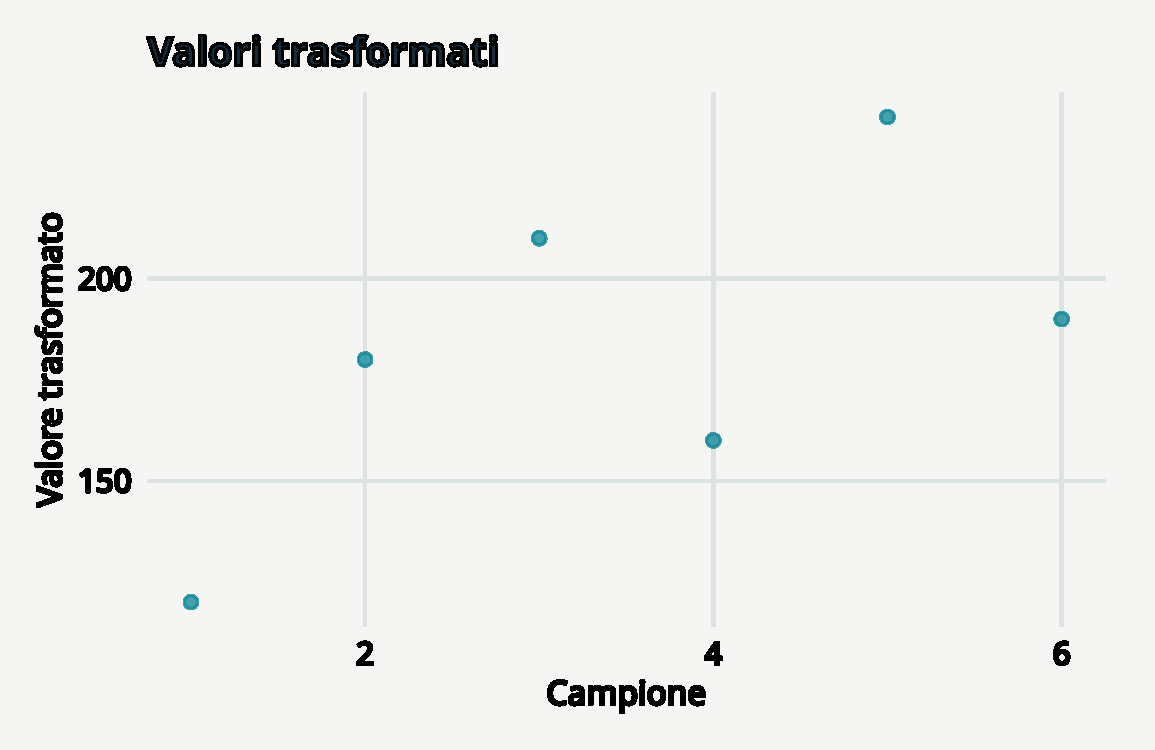
\includegraphics[width=\linewidth,height=6.0cm,keepaspectratio]{Esperimenti/t00-programma-A.pdf}\par}
\PSmall{Fattore di conversione: 1000. Seme: 17.}
}};
\node[anchor=north west,inner sep=0] at([xshift=10.85cm,yshift=-2.12cm]current page.north west){\Colonna{8.16cm}{\PLabel{Scenario A · simulazione}
\PBody{Il calcolo parte da un vettore di misure, al quale viene applicato un fattore comune di conversione. Poiché ogni elemento conserva la propria posizione, la tabella permette di seguire l’associazione fra valore iniziale e valore trasformato; il grafico rende visibile la variazione della scala numerica.}
\par\smallskip{\centering\adjustbox{max width=.98\linewidth}{$\displaystyle y_i=a x_i,\quad \bar y=a\bar x$}\par\smallskip}
\PSmall{$x_i$ è la misura iniziale del campione $i$; $a$ è il fattore di conversione; $y_i$ è il valore trasformato. Le barre indicano medie aritmetiche.}
}};
\node[anchor=north east,inner sep=0] at([xshift=17.1cm,yshift=-12.04cm]current page.north west){\fontsize{7.7}{9}\selectfont \href{https://marzione00.github.io/Lab_Geo/\#laboratorio/t00-programma}{\color{Classical}\bfseries Apri il laboratorio · t00-programma}};
\end{tikzpicture}\end{frame}

\begin{frame}[plain]\hypertarget{slide11}{}
\bookmark[level=1,page=11]{Confronto | Dal dato alla trasformazione}
\begin{tikzpicture}[remember picture,overlay]
\PilotChrome{Confronto | Dal dato alla trasformazione}{DALLA DOMANDA AL PROGRAMMA}{11}{Una trasformazione elementare permette di ricostruire il passaggio fra dato e risultato.}
\node[anchor=north west,inner sep=0] at([xshift=.96cm,yshift=-2.12cm]current page.north west){\Colonna{9.40cm}{{\centering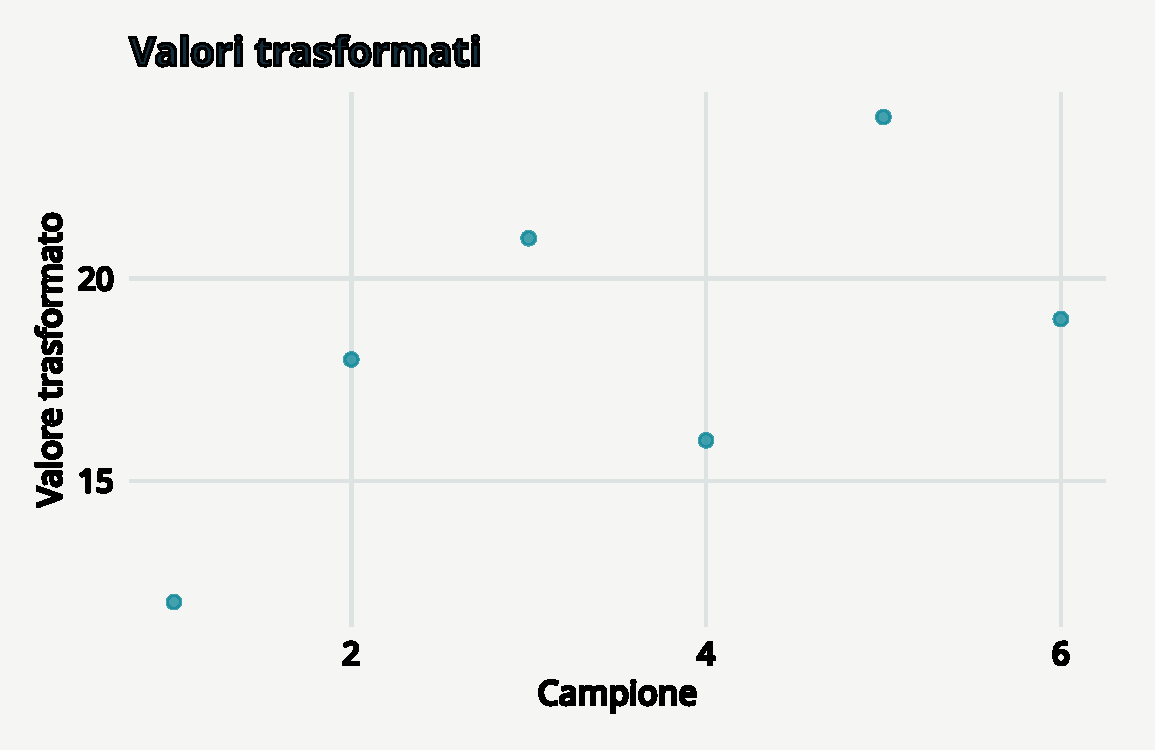
\includegraphics[width=\linewidth,height=5.6cm,keepaspectratio]{Esperimenti/t00-programma-B.pdf}\par}
\PSmall{Fattore di conversione: 1000 $\to$ 100. Tutti gli altri parametri e il seme sono fissi.}
}};
\node[anchor=north west,inner sep=0] at([xshift=10.85cm,yshift=-2.12cm]current page.north west){\Colonna{8.16cm}{\PLabel{Confronto fra gli scenari}
{\fontsize{10.2}{12.8}\selectfont\begin{tabular}{@{}>{\raggedright\arraybackslash}p{0.48\linewidth}@{\hspace{.13cm}}>{\raggedright\arraybackslash}p{0.224\linewidth}@{\hspace{.13cm}}>{\raggedright\arraybackslash}p{0.224\linewidth}@{}}\toprule Grandezza & A & B\\[2.3pt]
\midrule 
Media iniziale & 0,183 & 0,183\\[2.3pt]
Media trasformata & 183 & 18,3\\[2.3pt]
\bottomrule\end{tabular}\par}
\vspace{.25cm}\PBody{Moltiplicare per 100 anziché per 1000 riduce di dieci volte la media trasformata. La media di partenza resta 0,183.}
}};
\node[anchor=north east,inner sep=0] at([xshift=17.1cm,yshift=-12.04cm]current page.north west){\fontsize{7.7}{9}\selectfont \href{https://marzione00.github.io/Lab_Geo/\#laboratorio/t00-programma}{\color{Classical}\bfseries Apri il laboratorio · t00-programma}};
\end{tikzpicture}\end{frame}

\begin{frame}[plain]\hypertarget{slide12}{}
\bookmark[level=0,page=12]{Valori, tipi e operazioni}
\bookmark[level=1,page=12]{Una selezione deve conservare gli identificativi}
\begin{tikzpicture}[remember picture,overlay]
\PilotChrome{Una selezione deve conservare gli identificativi}{VALORI, TIPI E OPERAZIONI}{12}{La riga è l’unità da trasportare attraverso il filtro.}
\node[anchor=north west,inner sep=0] at([xshift=.96cm,yshift=-2.12cm]current page.north west){\Colonna{9.40cm}{\PLabel{Domanda}
\PBody{Il registro contiene una seconda misura per un provino. Selezionando le masse sopra 120 g, quali etichette accompagnano i numeri?}
\vspace{.35cm}\PLabel{Interpretazione}
\PBody{La maschera ha la stessa lunghezza delle due colonne. Applicandola a entrambe, C02 e C03 restano associati ai valori corretti.}
}};
\node[anchor=north west,inner sep=0] at([xshift=10.85cm,yshift=-2.12cm]current page.north west){\Colonna{8.16cm}{\begin{tcolorbox}[enhanced,arc=1.7mm,boxrule=.6pt,colback=white,colframe=Classical!60!Navy,colbacktitle=Navy,coltitle=white,fonttitle=\bfseries\small,title={R · calcolo riproducibile},left=1.7mm,right=1.3mm,top=1.1mm,bottom=1.1mm,before skip=1mm,after skip=1.0mm]\lstinputlisting[style=GeoR,language=R]{Codice/capitolo-02.R}\end{tcolorbox}
\PLabel{Risultato in R}
\begin{tcolorbox}[colback=GeoTint,colframe=Rule,boxrule=.5pt,arc=1.4mm,left=2mm,right=1mm,top=1mm,bottom=1mm]{\fontsize{9}{12}\selectfont\ttfamily \mbox{[1]\ "C02"\ "C03"}}\end{tcolorbox}}};
\end{tikzpicture}\end{frame}

\begin{frame}[plain]\hypertarget{slide13}{}
\bookmark[level=1,page=13]{La stessa operazione in R e Python}
\begin{tikzpicture}[remember picture,overlay]
\PilotChrome{La stessa operazione in R e Python}{VALORI, TIPI E OPERAZIONI}{13}{La maschera ha la stessa lunghezza delle due colonne. Applicandola a entrambe, C02 e C03 restano associati ai valori corretti.}
\node[anchor=north west,inner sep=0] at([xshift=.96cm,yshift=-2.12cm]current page.north west){\Colonna{9.40cm}{\begin{tcolorbox}[enhanced,arc=1.7mm,boxrule=.6pt,colback=white,colframe=Classical!60!Navy,colbacktitle=Navy,coltitle=white,fonttitle=\bfseries\small,title={R},left=1.7mm,right=1.3mm,top=1.1mm,bottom=1.1mm,before skip=1mm,after skip=1.0mm]\lstinputlisting[style=GeoR,language=R]{Codice/capitolo-02.R}\end{tcolorbox}
\PSmall{Caso: Una selezione deve conservare gli identificativi.}
}};
\node[anchor=north west,inner sep=0] at([xshift=10.85cm,yshift=-2.12cm]current page.north west){\Colonna{8.16cm}{\begin{tcolorbox}[enhanced,arc=1.7mm,boxrule=.6pt,colback=white,colframe=Classical!60!Navy,colbacktitle=Navy,coltitle=white,fonttitle=\bfseries\small,title={Python 3},left=1.7mm,right=1.3mm,top=1.1mm,bottom=1.1mm,before skip=1mm,after skip=1.0mm]\lstinputlisting[style=GeoR,language=Python]{Codice/capitolo-02.py}\end{tcolorbox}
\PInfo{La riga è l’unità da trasportare attraverso il filtro.}
}};
\end{tikzpicture}\end{frame}

\begin{frame}[plain]\hypertarget{slide14}{}
\bookmark[level=1,page=14]{La relazione fisica precede la sintassi}
\begin{tikzpicture}[remember picture,overlay]
\PilotChrome{La relazione fisica precede la sintassi}{VALORI, TIPI E OPERAZIONI}{14}{Il controllo manuale collega la formula, le unità e l’istruzione eseguita.}
\node[anchor=north west,inner sep=0] at([xshift=.96cm,yshift=-2.12cm]current page.north west){\Colonna{9.40cm}{\begin{tcolorbox}[enhanced,arc=1.7mm,boxrule=.6pt,colback=white,colframe=Classical!60!Navy,colbacktitle=Navy,coltitle=white,fonttitle=\bfseries\small,title={R · istruzioni},left=1.7mm,right=1.3mm,top=1.1mm,bottom=1.1mm,before skip=1mm,after skip=1.0mm]\lstinputlisting[style=GeoR,language=R]{Codice/lettura-07.R}\end{tcolorbox}
\par\smallskip{\centering\adjustbox{max width=.98\linewidth}{$\displaystyle \rho=\frac mV=\frac{107{,}2\ \mathrm g}{40\ \mathrm{cm}^3}=2{,}68\ \mathrm{g\,cm^{-3}}$}\par\smallskip}
}};
\node[anchor=north west,inner sep=0] at([xshift=10.85cm,yshift=-2.12cm]current page.north west){\Colonna{8.16cm}{\PBody{La densità del primo provino deriva dal rapporto fra 107,2 grammi e quaranta centimetri cubi, restituendo 2,68 grammi per centimetro cubo. Il codice conserva le unità nei nomi delle variabili e confronta il risultato con un calcolo manuale. In R la freccia assegna un valore, mentre il confronto di uguaglianza usa due segni uguali. In Python l’assegnazione usa un segno uguale e la medesima divisione esprime il rapporto, purché i valori siano numerici e le unità restino coerenti.}
}};
\end{tikzpicture}\end{frame}

\begin{frame}[plain]\hypertarget{slide15}{}
\bookmark[level=1,page=15]{Il tipo dell’oggetto determina l’operazione}
\begin{tikzpicture}[remember picture,overlay]
\PilotChrome{Il tipo dell’oggetto determina l’operazione}{VALORI, TIPI E OPERAZIONI}{15}{La lettura del codice richiede di conoscere sia l’operatore sia il tipo degli oggetti coinvolti.}
\node[anchor=north west,inner sep=0] at([xshift=.96cm,yshift=-2.12cm]current page.north west){\Colonna{9.40cm}{{\centering\resizebox{.97\linewidth}{!}{\begin{tikzpicture}[x=1cm,y=-.87cm,every node/.style={font=\fontsize{12.2}{15}\selectfont,text=Ink},arr/.style={-{Stealth[length=2mm]},line width=.8pt,draw=Classical}]\path[use as bounding box] (0,0) rectangle (7.45,6.2);
\draw[draw=Classical,fill=Classical!8,rounded corners=2pt,line width=.7pt] (0.25,0.3) rectangle (7.15,2.8);
\node[anchor=center,text=Classical,font=\fontsize{12.2}{15}\selectfont,text width=6.5cm,align=center] at (3.7,0.75) {\textbf{Lista Python}};
\node[anchor=center,text=Ink,font=\fontsize{13}{15}\selectfont,text width=2.5cm,align=center] at (1.85,1.55) {[1, 2]};
\draw[arr,draw=Classical] (3.1,1.55)--(3.8,1.55);
\node[anchor=center,text=Ink,font=\fontsize{13}{15}\selectfont,text width=3cm,align=center] at (5.45,1.55) {[1, 2, 1, 2]};
\node[anchor=center,text=Ink,font=\fontsize{11.5}{15}\selectfont,text width=6.5cm,align=center] at (3.7,2.35) {× 2 ripete gli elementi};
\draw[draw=Quantum,fill=Quantum!8,rounded corners=2pt,line width=.7pt] (0.25,3.25) rectangle (7.15,5.75);
\node[anchor=center,text=Quantum,font=\fontsize{12.2}{15}\selectfont,text width=6.5cm,align=center] at (3.7,3.7) {\textbf{Array NumPy}};
\node[anchor=center,text=Ink,font=\fontsize{13}{15}\selectfont,text width=2.5cm,align=center] at (1.85,4.5) {[1, 2]};
\draw[arr,draw=Quantum] (3.1,4.5)--(3.8,4.5);
\node[anchor=center,text=Ink,font=\fontsize{13}{15}\selectfont,text width=3cm,align=center] at (5.45,4.5) {[2, 4]};
\node[anchor=center,text=Ink,font=\fontsize{11.5}{15}\selectfont,text width=6.5cm,align=center] at (3.7,5.3) {× 2 raddoppia ogni valore};

\end{tikzpicture}}\par}
}};
\node[anchor=north west,inner sep=0] at([xshift=10.85cm,yshift=-2.12cm]current page.north west){\Colonna{8.16cm}{\PBody{Un vettore atomico R raccoglie valori di un tipo comune, mentre una tabella può associare colonne di tipi differenti. In Python, una lista e un array numerico interpretano diversamente alcune operazioni: moltiplicare una lista per due ne ripete gli elementi, mentre moltiplicare un array NumPy raddoppia i valori. Il simbolo scritto nel programma acquista pertanto significato attraverso il tipo degli operandi. La verifica di struttura e tipi dopo l’importazione evita che una misura venga trattata come testo o che un codice perda il proprio formato.}
}};
\end{tikzpicture}\end{frame}

\begin{frame}[plain]\hypertarget{slide16}{}
\bookmark[level=1,page=16]{Indici e corrispondenza delle righe}
\begin{tikzpicture}[remember picture,overlay]
\PilotChrome{Indici e corrispondenza delle righe}{VALORI, TIPI E OPERAZIONI}{16}{La verifica degli identificativi protegge la corrispondenza scientifica oltre la convenzione degli indici.}
\node[anchor=north west,inner sep=0] at([xshift=.96cm,yshift=-2.12cm]current page.north west){\Colonna{9.40cm}{{\centering\resizebox{.97\linewidth}{!}{\begin{tikzpicture}[x=1cm,y=-.87cm,every node/.style={font=\fontsize{12.2}{15}\selectfont,text=Ink},arr/.style={-{Stealth[length=2mm]},line width=.8pt,draw=Classical}]\path[use as bounding box] (0,0) rectangle (7.45,6.2);
\draw[draw=Classical,fill=Classical!8,rounded corners=2pt,line width=.7pt] (0.6,1.7) rectangle (2.4,3.3);
\node[anchor=center,text=Ink,font=\fontsize{13}{15}\selectfont,text width=1.6cm,align=center] at (1.5,2.5) {C01};
\node[anchor=center,text=Ink,font=\fontsize{12}{15}\selectfont] at (1.5,0.9) {R: 1};
\node[anchor=center,text=Ink,font=\fontsize{12}{15}\selectfont] at (1.5,4.1) {Python: 0};
\draw[draw=Classical,fill=Classical!8,rounded corners=2pt,line width=.7pt] (2.7,1.7) rectangle (4.5,3.3);
\node[anchor=center,text=Ink,font=\fontsize{13}{15}\selectfont,text width=1.6cm,align=center] at (3.6,2.5) {C02};
\node[anchor=center,text=Ink,font=\fontsize{12}{15}\selectfont] at (3.6,0.9) {R: 2};
\node[anchor=center,text=Ink,font=\fontsize{12}{15}\selectfont] at (3.6,4.1) {Python: 1};
\draw[draw=Classical,fill=Classical!8,rounded corners=2pt,line width=.7pt] (4.8,1.7) rectangle (6.6,3.3);
\node[anchor=center,text=Ink,font=\fontsize{13}{15}\selectfont,text width=1.6cm,align=center] at (5.7,2.5) {C03};
\node[anchor=center,text=Ink,font=\fontsize{12}{15}\selectfont] at (5.7,0.9) {R: 3};
\node[anchor=center,text=Ink,font=\fontsize{12}{15}\selectfont] at (5.7,4.1) {Python: 2};
\node[anchor=center,text=Ink,font=\fontsize{11}{15}\selectfont,text width=6.8cm,align=center] at (3.7,5.5) {Stessi provini, convenzioni di accesso differenti.};

\end{tikzpicture}}\par}
}};
\node[anchor=north west,inner sep=0] at([xshift=10.85cm,yshift=-2.12cm]current page.north west){\Colonna{8.16cm}{\PBody{Gli indici numerici ordinari di un vettore R iniziano da uno, mentre quelli di una lista o di un array Python iniziano da zero. Il primo elemento viene quindi richiamato con x[1] in R e x[0] in Python. La differenza riguarda la convenzione di accesso e lascia invariata l’identità dell’osservazione, purché l’ordine dei dati coincida. Negli scambi fra linguaggi conviene verificare gli identificativi, poiché la posizione nella tabella può cambiare dopo ordinamenti, filtri o aggregazioni.}
}};
\end{tikzpicture}\end{frame}

\begin{frame}[plain]\hypertarget{slide17}{}
\bookmark[level=1,page=17]{Operazioni vettoriali e controllo delle dimensioni}
\begin{tikzpicture}[remember picture,overlay]
\PilotChrome{Operazioni vettoriali e controllo delle dimensioni}{VALORI, TIPI E OPERAZIONI}{17}{La forma compatta di un’operazione conserva la necessità di verificare l’allineamento delle osservazioni.}
\node[anchor=north west,inner sep=0] at([xshift=.96cm,yshift=-2.12cm]current page.north west){\Colonna{9.40cm}{\begin{tcolorbox}[enhanced,arc=1.7mm,boxrule=.6pt,colback=white,colframe=Classical!60!Navy,colbacktitle=Navy,coltitle=white,fonttitle=\bfseries\small,title={R · procedura},left=1.7mm,right=1.3mm,top=1.1mm,bottom=1.1mm,before skip=1mm,after skip=1.0mm]\lstinputlisting[style=GeoR,language=R]{Codice/lettura-10.R}\end{tcolorbox}
\par\smallskip{\centering\adjustbox{max width=.98\linewidth}{$\displaystyle \rho_i=m_i/V_i,\qquad i=1,\ldots,n$}\par\smallskip}
}};
\node[anchor=north west,inner sep=0] at([xshift=10.85cm,yshift=-2.12cm]current page.north west){\Colonna{8.16cm}{\PBody{Per n provini, la divisione fra i vettori delle masse m e dei volumi V calcola una densità per ogni coppia, mantenendo l’associazione stabilita dall’ordine delle righe. In R vettori di lunghezze differenti possono essere riciclati, producendo talvolta un risultato numericamente plausibile ma privo della corrispondenza desiderata. Il controllo della lunghezza precede quindi l’operazione. Un ciclo esplicito può esprimere lo stesso algoritmo; la scelta fra ciclo e operazione vettoriale deve conservare significato, leggibilità e gestione dei casi limite.}
}};
\end{tikzpicture}\end{frame}

\begin{frame}[plain]\hypertarget{slide18}{}
\bookmark[level=1,page=18]{Tipi, vettori e selezioni}
\begin{tikzpicture}[remember picture,overlay]
\PilotChrome{Tipi, vettori e selezioni}{VALORI, TIPI E OPERAZIONI}{18}{Esaminare una selezione logica e la sua applicazione a un vettore.}
\node[anchor=north west,inner sep=0] at([xshift=.96cm,yshift=-2.12cm]current page.north west){\Colonna{9.40cm}{{\centering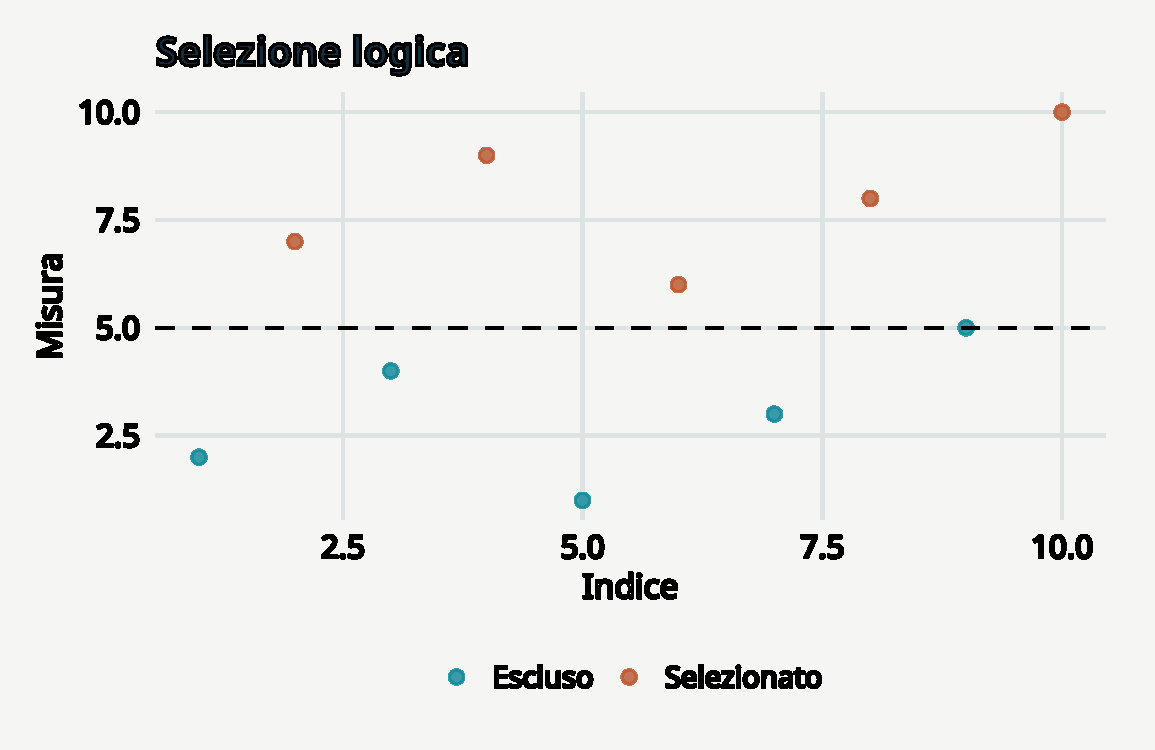
\includegraphics[width=\linewidth,height=6.0cm,keepaspectratio]{Esperimenti/t00-tipi-A.pdf}\par}
\PSmall{Soglia di selezione: 5. Seme: 17.}
}};
\node[anchor=north west,inner sep=0] at([xshift=10.85cm,yshift=-2.12cm]current page.north west){\Colonna{8.16cm}{\PLabel{Scenario A · simulazione}
\PBody{Una condizione applicata a un vettore produce un risultato logico per ciascuna osservazione. Nell’esperimento vengono selezionati i valori strettamente maggiori della soglia, mentre il grafico mantiene visibili anche quelli esclusi, affinché sia possibile ricostruire il cambiamento del campione analitico.}
\par\smallskip{\centering\adjustbox{max width=.98\linewidth}{$\displaystyle I_i=\mathbf{1}(x_i>c),\quad \bar x_I=\frac{\sum I_i x_i}{\sum I_i}$}\par\smallskip}
\PSmall{$c$ è la soglia; $I_i$ vale uno quando $x_i>c$ e zero altrimenti; $\bar x_I$ è la media delle sole osservazioni selezionate.}
}};
\node[anchor=north east,inner sep=0] at([xshift=17.1cm,yshift=-12.04cm]current page.north west){\fontsize{7.7}{9}\selectfont \href{https://marzione00.github.io/Lab_Geo/\#laboratorio/t00-tipi}{\color{Classical}\bfseries Apri il laboratorio · t00-tipi}};
\end{tikzpicture}\end{frame}

\begin{frame}[plain]\hypertarget{slide19}{}
\bookmark[level=1,page=19]{Confronto | Tipi, vettori e selezioni}
\begin{tikzpicture}[remember picture,overlay]
\PilotChrome{Confronto | Tipi, vettori e selezioni}{VALORI, TIPI E OPERAZIONI}{19}{La media riguarda soltanto le osservazioni selezionate; la dimensione del sottoinsieme va dichiarata.}
\node[anchor=north west,inner sep=0] at([xshift=.96cm,yshift=-2.12cm]current page.north west){\Colonna{9.40cm}{{\centering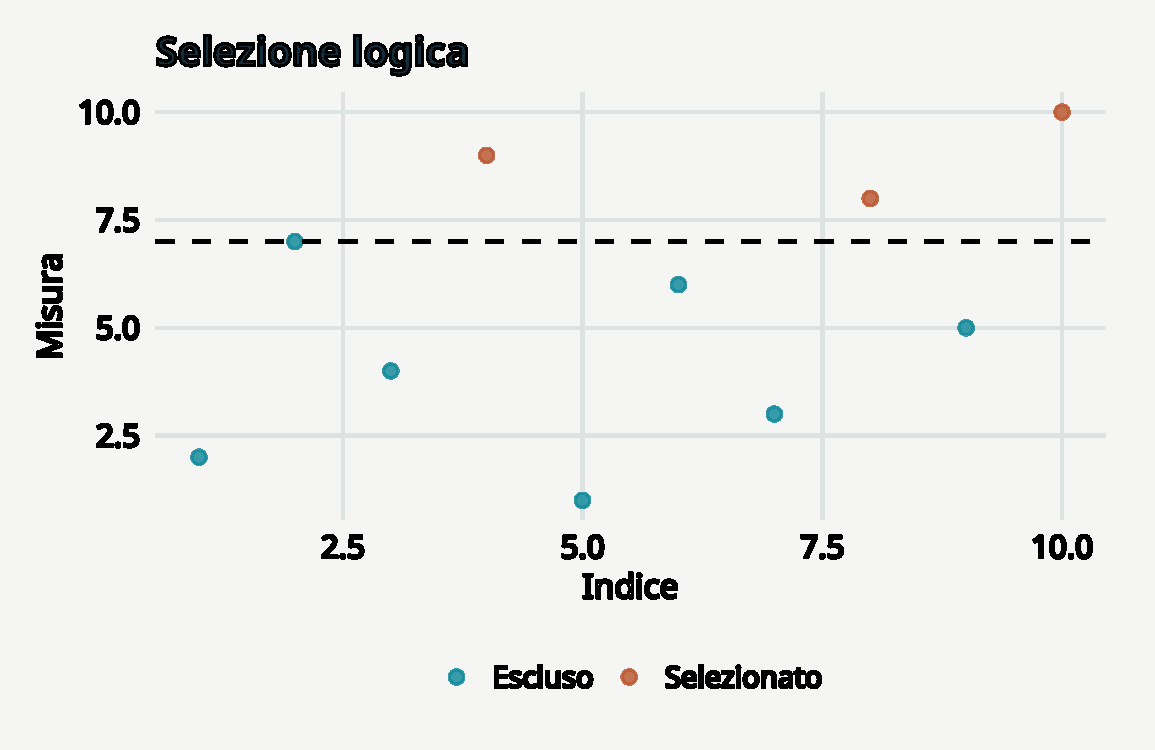
\includegraphics[width=\linewidth,height=5.6cm,keepaspectratio]{Esperimenti/t00-tipi-B.pdf}\par}
\PSmall{Soglia di selezione: 5 $\to$ 7. Tutti gli altri parametri e il seme sono fissi.}
}};
\node[anchor=north west,inner sep=0] at([xshift=10.85cm,yshift=-2.12cm]current page.north west){\Colonna{8.16cm}{\PLabel{Confronto fra gli scenari}
{\fontsize{10.2}{12.8}\selectfont\begin{tabular}{@{}>{\raggedright\arraybackslash}p{0.48\linewidth}@{\hspace{.13cm}}>{\raggedright\arraybackslash}p{0.224\linewidth}@{\hspace{.13cm}}>{\raggedright\arraybackslash}p{0.224\linewidth}@{}}\toprule Grandezza & A & B\\[2.3pt]
\midrule 
Selezionati & 5 & 3\\[2.3pt]
Media selezionata & 8 & 9\\[2.3pt]
\bottomrule\end{tabular}\par}
\vspace{.25cm}\PBody{Alzando la soglia da 5 a 7 entrano tre osservazioni anziché cinque. La media riguarda ora i valori più elevati.}
}};
\node[anchor=north east,inner sep=0] at([xshift=17.1cm,yshift=-12.04cm]current page.north west){\fontsize{7.7}{9}\selectfont \href{https://marzione00.github.io/Lab_Geo/\#laboratorio/t00-tipi}{\color{Classical}\bfseries Apri il laboratorio · t00-tipi}};
\end{tikzpicture}\end{frame}

\begin{frame}[plain]\hypertarget{slide20}{}
\bookmark[level=0,page=20]{Lettura e trasformazione dei dati}
\bookmark[level=1,page=20]{Una cella vuota cambia il denominatore}
\begin{tikzpicture}[remember picture,overlay]
\PilotChrome{Una cella vuota cambia il denominatore}{LETTURA E TRASFORMAZIONE DEI DATI}{20}{Conserva il numero di misure valide accanto alla sintesi.}
\node[anchor=north west,inner sep=0] at([xshift=.96cm,yshift=-2.12cm]current page.north west){\Colonna{9.40cm}{\PLabel{Domanda}
\PBody{Due volumi sono misurati, il terzo è assente. Che cosa cambierebbe sostituendo il dato assente con zero?}
\vspace{.35cm}\PLabel{Interpretazione}
\PBody{La media dei due volumi disponibili vale 45 cm³. Inserire zero produce 30 cm³ e attribuisce al terzo campione una misura mai eseguita.}
}};
\node[anchor=north west,inner sep=0] at([xshift=10.85cm,yshift=-2.12cm]current page.north west){\Colonna{8.16cm}{\begin{tcolorbox}[enhanced,arc=1.7mm,boxrule=.6pt,colback=white,colframe=Classical!60!Navy,colbacktitle=Navy,coltitle=white,fonttitle=\bfseries\small,title={R · calcolo riproducibile},left=1.7mm,right=1.3mm,top=1.1mm,bottom=1.1mm,before skip=1mm,after skip=1.0mm]\lstinputlisting[style=GeoR,language=R]{Codice/capitolo-03.R}\end{tcolorbox}
\PLabel{Risultato in R}
\begin{tcolorbox}[colback=GeoTint,colframe=Rule,boxrule=.5pt,arc=1.4mm,left=2mm,right=1mm,top=1mm,bottom=1mm]{\fontsize{9}{12}\selectfont\ttfamily \mbox{validi\ \ media\ }\\\mbox{\ \ \ \ \ 2\ \ \ \ \ 45}}\end{tcolorbox}}};
\end{tikzpicture}\end{frame}

\begin{frame}[plain]\hypertarget{slide21}{}
\bookmark[level=1,page=21]{La stessa operazione in R e Python}
\begin{tikzpicture}[remember picture,overlay]
\PilotChrome{La stessa operazione in R e Python}{LETTURA E TRASFORMAZIONE DEI DATI}{21}{La media dei due volumi disponibili vale 45 cm³. Inserire zero produce 30 cm³ e attribuisce al terzo campione una misura mai eseguita.}
\node[anchor=north west,inner sep=0] at([xshift=.96cm,yshift=-2.12cm]current page.north west){\Colonna{9.40cm}{\begin{tcolorbox}[enhanced,arc=1.7mm,boxrule=.6pt,colback=white,colframe=Classical!60!Navy,colbacktitle=Navy,coltitle=white,fonttitle=\bfseries\small,title={R},left=1.7mm,right=1.3mm,top=1.1mm,bottom=1.1mm,before skip=1mm,after skip=1.0mm]\lstinputlisting[style=GeoR,language=R]{Codice/capitolo-03.R}\end{tcolorbox}
\PSmall{Caso: Una cella vuota cambia il denominatore.}
}};
\node[anchor=north west,inner sep=0] at([xshift=10.85cm,yshift=-2.12cm]current page.north west){\Colonna{8.16cm}{\begin{tcolorbox}[enhanced,arc=1.7mm,boxrule=.6pt,colback=white,colframe=Classical!60!Navy,colbacktitle=Navy,coltitle=white,fonttitle=\bfseries\small,title={Python 3},left=1.7mm,right=1.3mm,top=1.1mm,bottom=1.1mm,before skip=1mm,after skip=1.0mm]\lstinputlisting[style=GeoR,language=Python]{Codice/capitolo-03.py}\end{tcolorbox}
\PInfo{Conserva il numero di misure valide accanto alla sintesi.}
}};
\end{tikzpicture}\end{frame}

\begin{frame}[plain]\hypertarget{slide22}{}
\bookmark[level=1,page=22]{Il CSV rappresenta testo organizzato in colonne}
\begin{tikzpicture}[remember picture,overlay]
\PilotChrome{Il CSV rappresenta testo organizzato in colonne}{LETTURA E TRASFORMAZIONE DEI DATI}{22}{L’importazione interpreta una rappresentazione e richiede convenzioni dichiarate.}
\node[anchor=north west,inner sep=0] at([xshift=.96cm,yshift=-2.12cm]current page.north west){\Colonna{9.40cm}{{\centering\resizebox{.97\linewidth}{!}{\begin{tikzpicture}[x=1cm,y=-.87cm,every node/.style={font=\fontsize{12.2}{15}\selectfont,text=Ink},arr/.style={-{Stealth[length=2mm]},line width=.8pt,draw=Classical}]\path[use as bounding box] (0,0) rectangle (7.45,6.2);
\draw[draw=Classical,fill=Classical!8,rounded corners=2pt,line width=.7pt] (0.25,0.25) rectangle (7.15,1.6);
\node[anchor=center,text=Classical,font=\fontsize{12}{15}\selectfont,text width=6.5cm,align=center] at (3.7,0.61) {\textbf{File di testo}};
\node[anchor=center,text=Ink,font=\fontsize{11.3}{15}\selectfont,text width=6.5cm,align=center] at (3.7,1.2) {Caratteri e separatori};
\draw[arr,draw=Classical] (3.7,1.65)--(3.7,1.97);
\draw[draw=Quantum,fill=Quantum!8,rounded corners=2pt,line width=.7pt] (0.25,2.1) rectangle (7.15,3.45);
\node[anchor=center,text=Quantum,font=\fontsize{12}{15}\selectfont,text width=6.5cm,align=center] at (3.7,2.46) {\textbf{Lettura}};
\node[anchor=center,text=Ink,font=\fontsize{11.3}{15}\selectfont,text width=6.5cm,align=center] at (3.7,3.05) {Codifica, separatori e tipi};
\draw[arr,draw=Quantum] (3.7,3.5)--(3.7,3.8200000000000003);
\draw[draw=Classical,fill=Classical!8,rounded corners=2pt,line width=.7pt] (0.25,3.95) rectangle (7.15,5.300000000000001);
\node[anchor=center,text=Classical,font=\fontsize{12}{15}\selectfont,text width=6.5cm,align=center] at (3.7,4.3100000000000005) {\textbf{Tabella}};
\node[anchor=center,text=Ink,font=\fontsize{11.3}{15}\selectfont,text width=6.5cm,align=center] at (3.7,4.9) {Valori organizzati in righe e colonne};

\end{tikzpicture}}\par}
}};
\node[anchor=north west,inner sep=0] at([xshift=10.85cm,yshift=-2.12cm]current page.north west){\Colonna{8.16cm}{\PBody{Un file CSV contiene caratteri, separatori e righe che il programma interpreta secondo regole di lettura. Il separatore decimale, il simbolo dei mancanti e la codifica dei caratteri incidono sulla ricostruzione della tabella. Un identificativo come 001 deve essere conservato come testo quando gli zeri iniziali fanno parte del codice. Il formato tabellare richiede un dizionario esterno per documentare unità, metodi e significato delle colonne, poiché tali informazioni non sono garantite dalla sola estensione del file.}
}};
\end{tikzpicture}\end{frame}

\begin{frame}[plain]\hypertarget{slide23}{}
\bookmark[level=1,page=23]{Controlli iniziali e cartella di avvio}
\begin{tikzpicture}[remember picture,overlay]
\PilotChrome{Controlli iniziali e cartella di avvio}{LETTURA E TRASFORMAZIONE DEI DATI}{23}{Il controllo dell’input distingue problemi di accesso, struttura e contenuto prima del calcolo.}
\node[anchor=north west,inner sep=0] at([xshift=.96cm,yshift=-2.12cm]current page.north west){\Colonna{9.40cm}{\begin{tcolorbox}[enhanced,arc=1.7mm,boxrule=.6pt,colback=white,colframe=Classical!60!Navy,colbacktitle=Navy,coltitle=white,fonttitle=\bfseries\small,title={R · procedura},left=1.7mm,right=1.3mm,top=1.1mm,bottom=1.1mm,before skip=1mm,after skip=1.0mm]\lstinputlisting[style=GeoR,language=R]{Codice/lettura-12.R}\end{tcolorbox}
}};
\node[anchor=north west,inner sep=0] at([xshift=10.85cm,yshift=-2.12cm]current page.north west){\Colonna{8.16cm}{\PBody{Il frammento assume che la sessione sia avviata dalla radice del progetto e cerca il CSV nella cartella dati. Dopo la lettura verifica ventiquattro righe, identificativi unici, massa numerica e volumi finiti positivi. L’ispezione della struttura completa questi controlli mostrando i tipi assegnati alle colonne. Se il file risulta assente, si esaminano cartella corrente, nome ed estensione prima di modificare il codice di analisi; un errore di percorso riguarda infatti l’accesso al dato e precede qualsiasi problema statistico.}
}};
\end{tikzpicture}\end{frame}

\begin{frame}[plain]\hypertarget{slide24}{}
\bookmark[level=1,page=24]{Filtrare conservando l’unità della riga}
\begin{tikzpicture}[remember picture,overlay]
\PilotChrome{Filtrare conservando l’unità della riga}{LETTURA E TRASFORMAZIONE DEI DATI}{24}{L’identità del provino resta il riferimento di ogni trasformazione della tabella.}
\node[anchor=north west,inner sep=0] at([xshift=.96cm,yshift=-2.12cm]current page.north west){\Colonna{9.40cm}{{\centering\resizebox{.97\linewidth}{!}{\begin{tikzpicture}[x=1cm,y=-.87cm,every node/.style={font=\fontsize{12.2}{15}\selectfont,text=Ink},arr/.style={-{Stealth[length=2mm]},line width=.8pt,draw=Classical}]\path[use as bounding box] (0,0) rectangle (7.45,6.2);
\node[anchor=center,text=Ink,font=\fontsize{12.5}{15}\selectfont,text width=7cm,align=center] at (3.7,0.45) {\textbf{Condizione: }$V\geq45\ \mathrm{cm}^3$};
\draw[draw=Muted,fill=Muted!4,rounded corners=2pt,line width=.7pt] (0.25,1.1) rectangle (7.15,2.2800000000000002);
\node[anchor=center,text=Muted,font=\fontsize{11}{15}\selectfont,text width=6.7cm,align=center] at (3.7,1.4200000000000002) {C01 · A1 · 107,2 g · 40 cm³};
\node[anchor=center,text=Muted,font=\fontsize{11}{15}\selectfont,text width=6.7cm,align=center] at (3.7,1.94) {escluso};
\draw[draw=Classical,fill=Classical!10,rounded corners=2pt,line width=.7pt] (0.25,2.55) rectangle (7.15,3.7299999999999995);
\node[anchor=center,text=Classical,font=\fontsize{11}{15}\selectfont,text width=6.7cm,align=center] at (3.7,2.8699999999999997) {C02 · A1 · 121,95 g · 45 cm³};
\node[anchor=center,text=Classical,font=\fontsize{11}{15}\selectfont,text width=6.7cm,align=center] at (3.7,3.3899999999999997) {incluso};
\draw[draw=Classical,fill=Classical!10,rounded corners=2pt,line width=.7pt] (0.25,4.0) rectangle (7.15,5.18);
\node[anchor=center,text=Classical,font=\fontsize{11}{15}\selectfont,text width=6.7cm,align=center] at (3.7,4.32) {C03 · A1 · 132,5 g · 50 cm³};
\node[anchor=center,text=Classical,font=\fontsize{11}{15}\selectfont,text width=6.7cm,align=center] at (3.7,4.84) {incluso};
\node[anchor=center,text=Ink,font=\fontsize{12}{15}\selectfont,text width=7cm,align=center] at (3.7,5.85) {$A=\{2,3\}$: due righe complete};

\end{tikzpicture}}\par}
}};
\node[anchor=north west,inner sep=0] at([xshift=10.85cm,yshift=-2.12cm]current page.north west){\Colonna{8.16cm}{\PBody{Un filtro seleziona righe intere, preservando l’associazione fra identificativo id, massa m, volume V e stazione s. Indichiamo con A l’insieme degli indici che soddisfano la condizione e con $D_A$ la tabella risultante. Nell’esempio si conservano i provini con volume almeno pari a 45 centimetri cubi. Ordinare separatamente le colonne distruggerebbe la corrispondenza fra misure dello stesso provino; il confronto degli identificativi e il conteggio delle righe permettono invece di verificare l’effetto della selezione.}
\par\smallskip{\centering\adjustbox{max width=.98\linewidth}{$\displaystyle D_A=\{(id_i,m_i,V_i,s_i):i\in A\}$}\par\smallskip}
}};
\end{tikzpicture}\end{frame}

\begin{frame}[plain]\hypertarget{slide25}{}
\bookmark[level=1,page=25]{Valore mancante e osservazione censurata}
\begin{tikzpicture}[remember picture,overlay]
\PilotChrome{Valore mancante e osservazione censurata}{LETTURA E TRASFORMAZIONE DEI DATI}{25}{Codici di assenza e limiti di misura conservano informazioni diverse sul processo osservativo.}
\node[anchor=north west,inner sep=0] at([xshift=.96cm,yshift=-2.12cm]current page.north west){\Colonna{9.40cm}{\PLabel{Metodo}
\PBody{Un valore registrato come inferiore a 0,05 informa che la misura ricade sotto un limite, mentre un valore mancante segnala l’assenza dell’informazione secondo il protocollo adottato. La sostituzione automatica con zero cancellerebbe questa distinzione e introdurrebbe un valore esatto non osservato. Il dataset analitico dovrebbe conservare valore, limite e indicatore di censura in campi distinti. Nei calcoli introduttivi, la gestione di NA viene resa esplicita e collegata al numero di osservazioni effettivamente utilizzate.}
}};
\node[anchor=north west,inner sep=0] at([xshift=10.85cm,yshift=-2.12cm]current page.north west){\Colonna{8.16cm}{\PLabel{Interpretazione}
\PBody{Per x = c(1, NA, 3), mean(x) restituisce NA, mentre mean(x, na.rm = TRUE) restituisce 2 sui due valori disponibili. L’esclusione è computazionalmente definita; la sua pertinenza dipende dal motivo per cui manca la misura e dalla popolazione che si vuole descrivere.}
}};
\end{tikzpicture}\end{frame}

\begin{frame}[plain]\hypertarget{slide26}{}
\bookmark[level=1,page=26]{La variabile derivata conserva le osservazioni}
\begin{tikzpicture}[remember picture,overlay]
\PilotChrome{La variabile derivata conserva le osservazioni}{LETTURA E TRASFORMAZIONE DEI DATI}{26}{Una variabile derivata si interpreta insieme alle misure originarie e al disegno di campionamento.}
\node[anchor=north west,inner sep=0] at([xshift=.96cm,yshift=-2.12cm]current page.north west){\Colonna{9.40cm}{{\centering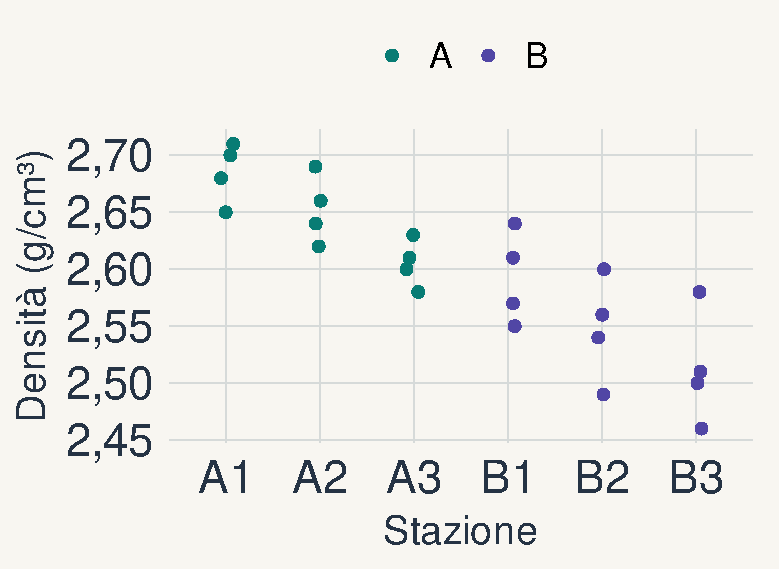
\includegraphics[width=\linewidth,height=6.15cm,keepaspectratio]{Figure/F02.pdf}\par}
\PSmall{Densità individuali ordinate per stazione. Il colore mantiene l’affioramento e rende visibile la struttura del campione.}
}};
\node[anchor=north west,inner sep=0] at([xshift=10.85cm,yshift=-2.12cm]current page.north west){\Colonna{8.16cm}{\PBody{La nuova colonna di densità viene calcolata per ciascun provino, lasciando disponibili massa e volume originari. Il grafico per stazione permette di riconoscere il raggruppamento dei dati e la variabilità fra provini dello stesso luogo. La lieve separazione orizzontale dei punti facilita la lettura senza modificare la densità rappresentata sull’asse verticale. Prima di sintetizzare le differenze fra affioramenti occorre mantenere evidente che le ventiquattro righe appartengono a sei unità geografiche distinte.}
}};
\end{tikzpicture}\end{frame}

\begin{frame}[plain]\hypertarget{slide27}{}
\bookmark[level=1,page=27]{Media dei rapporti e rapporto delle somme}
\begin{tikzpicture}[remember picture,overlay]
\PilotChrome{Media dei rapporti e rapporto delle somme}{LETTURA E TRASFORMAZIONE DEI DATI}{27}{L’aggregazione incorpora una ponderazione che deve essere coerente con la domanda fisica.}
\node[anchor=north west,inner sep=0] at([xshift=.96cm,yshift=-2.12cm]current page.north west){\Colonna{9.40cm}{\PLabel{Metodo}
\PBody{Per n provini, con masse $m_i$ e volumi $V_i$, la media delle densità attribuisce uguale peso a ciascun provino; il rapporto fra massa totale e volume totale assegna invece pesi $w_i$ proporzionali ai volumi. Le due quantità valgono qui circa 2,59917 e 2,59984 grammi per centimetro cubo. La vicinanza numerica dipende da questi dati, mentre la diversa ponderazione corrisponde a due distinti significati fisici.}
}};
\node[anchor=north west,inner sep=0] at([xshift=10.85cm,yshift=-2.12cm]current page.north west){\Colonna{8.16cm}{\PLabel{Formalismo}
\par\smallskip{\centering\adjustbox{max width=.98\linewidth}{$\displaystyle \overline\rho=\frac1n\sum_i\frac{m_i}{V_i},\qquad\rho_{tot}=\frac{\sum_i m_i}{\sum_i V_i}$}\par\smallskip}

\par\smallskip{\centering\adjustbox{max width=.98\linewidth}{$\displaystyle \rho_{tot}=\sum_i w_i\rho_i,\qquad w_i=\frac{V_i}{\sum_j V_j}$}\par\smallskip}
\PLabel{Interpretazione}
\PBody{La prima sintesi descrive il provino medio secondo pesi uguali. La seconda descrive il rapporto complessivo del materiale considerato, sotto una somma di volumi pertinente al problema. La scelta deve precedere l’interpretazione delle differenze fra gruppi.}
}};
\end{tikzpicture}\end{frame}

\begin{frame}[plain]\hypertarget{slide28}{}
\bookmark[level=1,page=28]{Sintesi per affioramento e livello dell’inferenza}
\begin{tikzpicture}[remember picture,overlay]
\PilotChrome{Sintesi per affioramento e livello dell’inferenza}{LETTURA E TRASFORMAZIONE DEI DATI}{28}{La sintesi descrittiva conserva un dominio osservativo che l’inferenza deve esplicitare.}
\node[anchor=north west,inner sep=0] at([xshift=.96cm,yshift=-2.12cm]current page.north west){\Colonna{9.40cm}{{\centering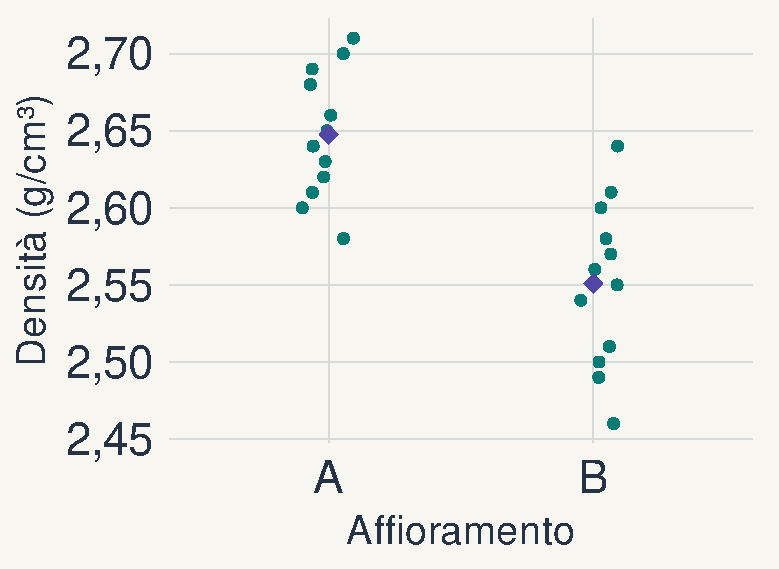
\includegraphics[width=\linewidth,height=6.15cm,keepaspectratio]{Figure/F03.pdf}\par}
\PSmall{Punti verdi: densità individuali. Rombi viola: medie per affioramento sui provini disponibili.}
}};
\node[anchor=north west,inner sep=0] at([xshift=10.85cm,yshift=-2.12cm]current page.north west){\Colonna{8.16cm}{\PBody{Le medie dei dodici provini dell’affioramento A e dei dodici dell’affioramento B sono rispettivamente 2,6475 e circa 2,55083 grammi per centimetro cubo. La figura conserva i valori individuali affinché la sintesi resti collegata alla dispersione osservata. Queste medie descrivono il campione disponibile; un confronto inferenziale richiederà di considerare le tre stazioni per affioramento, la dipendenza dei provini e il modo in cui i luoghi sono stati selezionati. Il calcolo corretto costituisce dunque un passaggio della costruzione dell’argomento scientifico.}
}};
\end{tikzpicture}\end{frame}

\begin{frame}[plain]\hypertarget{slide29}{}
\bookmark[level=1,page=29]{Dalla tabella alla sintesi}
\begin{tikzpicture}[remember picture,overlay]
\PilotChrome{Dalla tabella alla sintesi}{LETTURA E TRASFORMAZIONE DEI DATI}{29}{Confrontare aggregazioni ottenute da misure appartenenti a gruppi.}
\node[anchor=north west,inner sep=0] at([xshift=.96cm,yshift=-2.12cm]current page.north west){\Colonna{9.40cm}{{\centering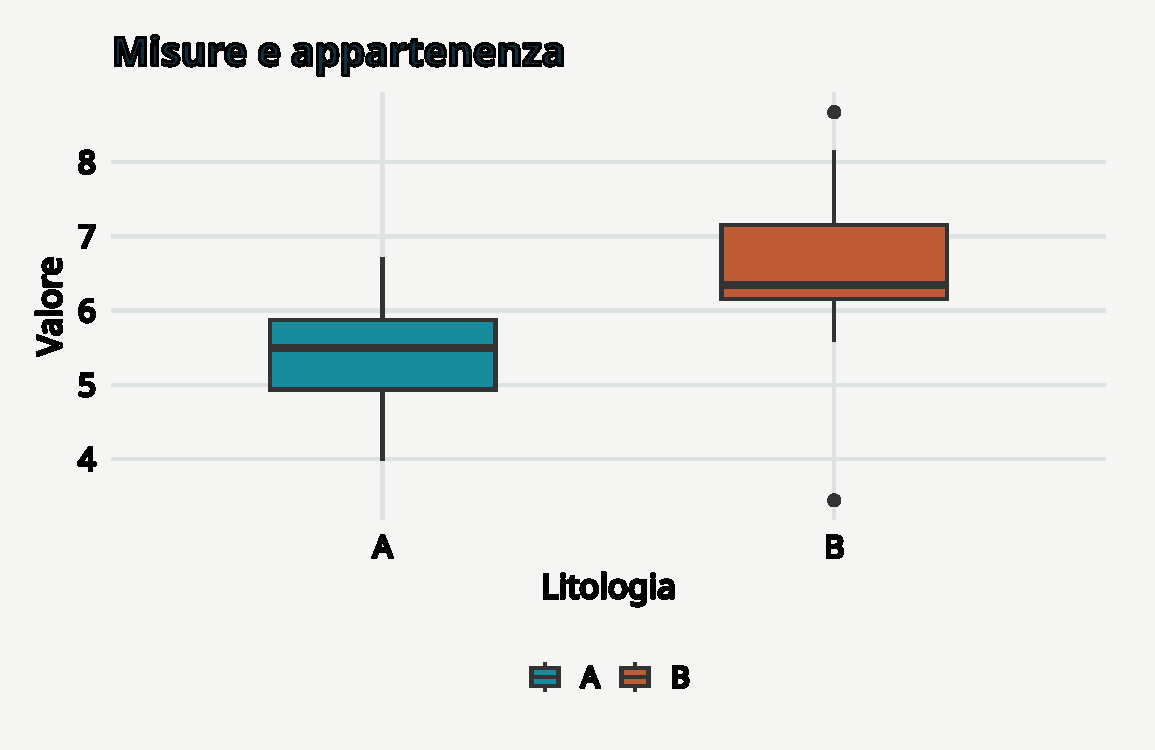
\includegraphics[width=\linewidth,height=6.0cm,keepaspectratio]{Esperimenti/t00-lettura-A.pdf}\par}
\PSmall{Differenza fra litologie: 2. Seme: 17.}
}};
\node[anchor=north west,inner sep=0] at([xshift=10.85cm,yshift=-2.12cm]current page.north west){\Colonna{8.16cm}{\PLabel{Scenario A · simulazione}
\PBody{La tabella contiene misure simulate appartenenti a due litologie, per le quali il modello assume distribuzioni normali con uguale dispersione. Il controllo della differenza sposta la media della seconda litologia, lasciando invariata la struttura della tabella e consentendo di confrontare direttamente le sintesi dei gruppi.}
\par\smallskip{\centering\adjustbox{max width=.98\linewidth}{$\displaystyle \bar x_g=n_g^{-1}\sum_{i\in g}x_i$}\par\smallskip}
\PSmall{$g$ identifica la litologia; $n_g$ è il numero delle sue osservazioni; $\bar x_g$ è la media dei valori appartenenti al gruppo.}
}};
\node[anchor=north east,inner sep=0] at([xshift=17.1cm,yshift=-12.04cm]current page.north west){\fontsize{7.7}{9}\selectfont \href{https://marzione00.github.io/Lab_Geo/\#laboratorio/t00-lettura}{\color{Classical}\bfseries Apri il laboratorio · t00-lettura}};
\end{tikzpicture}\end{frame}

\begin{frame}[plain]\hypertarget{slide30}{}
\bookmark[level=1,page=30]{Confronto | Dalla tabella alla sintesi}
\begin{tikzpicture}[remember picture,overlay]
\PilotChrome{Confronto | Dalla tabella alla sintesi}{LETTURA E TRASFORMAZIONE DEI DATI}{30}{Una tabella analitica conserva le informazioni necessarie a distinguere le unità di osservazione.}
\node[anchor=north west,inner sep=0] at([xshift=.96cm,yshift=-2.12cm]current page.north west){\Colonna{9.40cm}{{\centering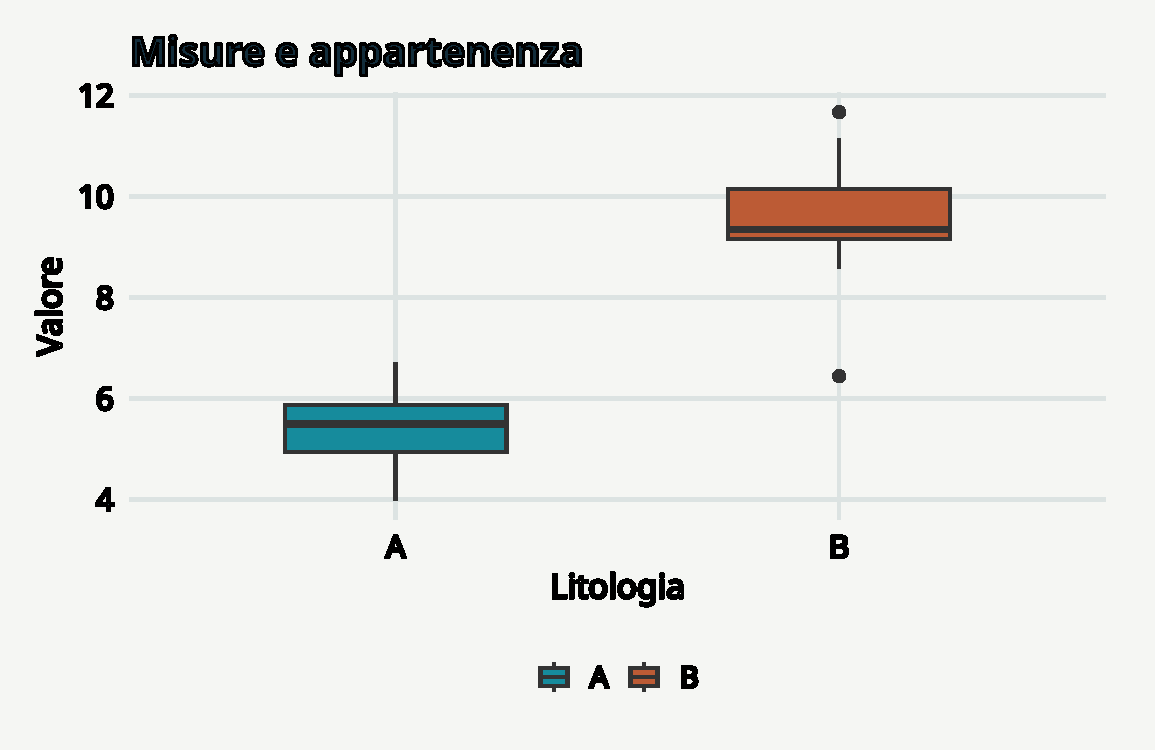
\includegraphics[width=\linewidth,height=5.6cm,keepaspectratio]{Esperimenti/t00-lettura-B.pdf}\par}
\PSmall{Differenza fra litologie: 2 $\to$ 5. Tutti gli altri parametri e il seme sono fissi.}
}};
\node[anchor=north west,inner sep=0] at([xshift=10.85cm,yshift=-2.12cm]current page.north west){\Colonna{8.16cm}{\PLabel{Confronto fra gli scenari}
{\fontsize{10.2}{12.8}\selectfont\begin{tabular}{@{}>{\raggedright\arraybackslash}p{0.48\linewidth}@{\hspace{.13cm}}>{\raggedright\arraybackslash}p{0.224\linewidth}@{\hspace{.13cm}}>{\raggedright\arraybackslash}p{0.224\linewidth}@{}}\toprule Grandezza & A & B\\[2.3pt]
\midrule 
Media A & 5,44 & 5,44\\[2.3pt]
Media B & 6,55 & 9,55\\[2.3pt]
\bottomrule\end{tabular}\par}
\vspace{.25cm}\PBody{Nel caso B la differenza generatrice aumenta di tre unità. Il gruppo di riferimento mantiene la stessa media perché il seme è fissato.}
}};
\node[anchor=north east,inner sep=0] at([xshift=17.1cm,yshift=-12.04cm]current page.north west){\fontsize{7.7}{9}\selectfont \href{https://marzione00.github.io/Lab_Geo/\#laboratorio/t00-lettura}{\color{Classical}\bfseries Apri il laboratorio · t00-lettura}};
\end{tikzpicture}\end{frame}

\begin{frame}[plain]\hypertarget{slide31}{}
\bookmark[level=0,page=31]{Errori e controllo del procedimento}
\bookmark[level=1,page=31]{Un valore noto mette alla prova la funzione}
\begin{tikzpicture}[remember picture,overlay]
\PilotChrome{Un valore noto mette alla prova la funzione}{ERRORI E CONTROLLO DEL PROCEDIMENTO}{31}{Un controllo sul significato del risultato completa il controllo sulla sintassi.}
\node[anchor=north west,inner sep=0] at([xshift=.96cm,yshift=-2.12cm]current page.north west){\Colonna{9.40cm}{\PLabel{Domanda}
\PBody{Un provino da 100 g con volume di 40 cm³ offre un risultato calcolabile a mano. Come lo useresti per verificare il codice?}
\vspace{.35cm}\PLabel{Interpretazione}
\PBody{Se si inverte il rapporto si ottiene 0,4. Il confronto con 2,5 scopre l’inversione anche quando il programma termina regolarmente.}
}};
\node[anchor=north west,inner sep=0] at([xshift=10.85cm,yshift=-2.12cm]current page.north west){\Colonna{8.16cm}{\begin{tcolorbox}[enhanced,arc=1.7mm,boxrule=.6pt,colback=white,colframe=Classical!60!Navy,colbacktitle=Navy,coltitle=white,fonttitle=\bfseries\small,title={R · calcolo riproducibile},left=1.7mm,right=1.3mm,top=1.1mm,bottom=1.1mm,before skip=1mm,after skip=1.0mm]\lstinputlisting[style=GeoR,language=R]{Codice/capitolo-04.R}\end{tcolorbox}
\PLabel{Risultato in R}
\begin{tcolorbox}[colback=GeoTint,colframe=Rule,boxrule=.5pt,arc=1.4mm,left=2mm,right=1mm,top=1mm,bottom=1mm]{\fontsize{9}{12}\selectfont\ttfamily \mbox{[1]\ TRUE}}\end{tcolorbox}}};
\end{tikzpicture}\end{frame}

\begin{frame}[plain]\hypertarget{slide32}{}
\bookmark[level=1,page=32]{La stessa operazione in R e Python}
\begin{tikzpicture}[remember picture,overlay]
\PilotChrome{La stessa operazione in R e Python}{ERRORI E CONTROLLO DEL PROCEDIMENTO}{32}{Se si inverte il rapporto si ottiene 0,4. Il confronto con 2,5 scopre l’inversione anche quando il programma termina regolarmente.}
\node[anchor=north west,inner sep=0] at([xshift=.96cm,yshift=-2.12cm]current page.north west){\Colonna{9.40cm}{\begin{tcolorbox}[enhanced,arc=1.7mm,boxrule=.6pt,colback=white,colframe=Classical!60!Navy,colbacktitle=Navy,coltitle=white,fonttitle=\bfseries\small,title={R},left=1.7mm,right=1.3mm,top=1.1mm,bottom=1.1mm,before skip=1mm,after skip=1.0mm]\lstinputlisting[style=GeoR,language=R]{Codice/capitolo-04.R}\end{tcolorbox}
\PSmall{Caso: Un valore noto mette alla prova la funzione.}
}};
\node[anchor=north west,inner sep=0] at([xshift=10.85cm,yshift=-2.12cm]current page.north west){\Colonna{8.16cm}{\begin{tcolorbox}[enhanced,arc=1.7mm,boxrule=.6pt,colback=white,colframe=Classical!60!Navy,colbacktitle=Navy,coltitle=white,fonttitle=\bfseries\small,title={Python 3},left=1.7mm,right=1.3mm,top=1.1mm,bottom=1.1mm,before skip=1mm,after skip=1.0mm]\lstinputlisting[style=GeoR,language=Python]{Codice/capitolo-04.py}\end{tcolorbox}
\PInfo{Un controllo sul significato del risultato completa il controllo sulla sintassi.}
}};
\end{tikzpicture}\end{frame}

\begin{frame}[plain]\hypertarget{slide33}{}
\bookmark[level=1,page=33]{Localizzare un errore attraverso il passaggio}
\begin{tikzpicture}[remember picture,overlay]
\PilotChrome{Localizzare un errore attraverso il passaggio}{ERRORI E CONTROLLO DEL PROCEDIMENTO}{33}{La riuscita tecnica dell’esecuzione deve essere accompagnata dall’esame della pertinenza del metodo.}
\node[anchor=north west,inner sep=0] at([xshift=.96cm,yshift=-2.12cm]current page.north west){\Colonna{9.40cm}{{\centering\resizebox{.97\linewidth}{!}{\begin{tikzpicture}[x=1cm,y=-.87cm,every node/.style={font=\fontsize{12.2}{15}\selectfont,text=Ink},arr/.style={-{Stealth[length=2mm]},line width=.8pt,draw=Classical}]\path[use as bounding box] (0,0) rectangle (7.45,6.2);
\draw[draw=Classical,fill=Classical!8,rounded corners=2pt,line width=.7pt] (0.25,0.25) rectangle (7.15,1.6);
\node[anchor=center,text=Classical,font=\fontsize{12}{15}\selectfont,text width=6.5cm,align=center] at (3.7,0.61) {\textbf{Sintassi}};
\node[anchor=center,text=Ink,font=\fontsize{11.3}{15}\selectfont,text width=6.5cm,align=center] at (3.7,1.2) {Le istruzioni sono interpretabili?};
\draw[arr,draw=Classical] (3.7,1.65)--(3.7,1.97);
\draw[draw=Quantum,fill=Quantum!8,rounded corners=2pt,line width=.7pt] (0.25,2.1) rectangle (7.15,3.45);
\node[anchor=center,text=Quantum,font=\fontsize{12}{15}\selectfont,text width=6.5cm,align=center] at (3.7,2.46) {\textbf{Esecuzione}};
\node[anchor=center,text=Ink,font=\fontsize{11.3}{15}\selectfont,text width=6.5cm,align=center] at (3.7,3.05) {Le operazioni sono definite?};
\draw[arr,draw=Quantum] (3.7,3.5)--(3.7,3.8200000000000003);
\draw[draw=Classical,fill=Classical!8,rounded corners=2pt,line width=.7pt] (0.25,3.95) rectangle (7.15,5.300000000000001);
\node[anchor=center,text=Classical,font=\fontsize{12}{15}\selectfont,text width=6.5cm,align=center] at (3.7,4.3100000000000005) {\textbf{Metodo}};
\node[anchor=center,text=Ink,font=\fontsize{11.3}{15}\selectfont,text width=6.5cm,align=center] at (3.7,4.9) {Il risultato risponde alla domanda?};

\end{tikzpicture}}\par}
}};
\node[anchor=north west,inner sep=0] at([xshift=10.85cm,yshift=-2.12cm]current page.north west){\Colonna{8.16cm}{\PBody{Un errore di sintassi impedisce di interpretare correttamente le istruzioni; un errore durante l’esecuzione interrompe un’operazione; un errore metodologico può produrre un risultato plausibile e completare il programma. La diagnosi segue quindi la sequenza dell’analisi, verificando file letto, struttura, condizioni del calcolo e significato della sintesi. Un esempio ridotto facilita l’identificazione del passaggio responsabile. Dopo la correzione si ripete l’esecuzione completa da una sessione pulita, per verificare che il risultato dipenda soltanto dagli input dichiarati.}
}};
\end{tikzpicture}\end{frame}

\begin{frame}[plain]\hypertarget{slide34}{}
\bookmark[level=1,page=34]{Funzioni piccole e valori di riferimento}
\begin{tikzpicture}[remember picture,overlay]
\PilotChrome{Funzioni piccole e valori di riferimento}{ERRORI E CONTROLLO DEL PROCEDIMENTO}{34}{Una funzione verificabile rende espliciti input, dominio e risultato atteso.}
\node[anchor=north west,inner sep=0] at([xshift=.96cm,yshift=-2.12cm]current page.north west){\Colonna{9.40cm}{\PLabel{Metodo}
\PBody{Una funzione raccoglie un’operazione definita attraverso argomenti e risultato, rendendo possibile verificarla separatamente dal resto dell’analisi. La funzione di densità richiede volumi positivi e associa masse e volumi della stessa lunghezza. La divisione di 107,2 g per 40 cm³ deve restituire 2,68 g/cm³; un volume nullo verifica il comportamento al limite del dominio. Separare importazione, trasformazione e scrittura permette di riutilizzare il calcolo senza incorporare dipendenze nascoste da file o oggetti della sessione.}
}};
\node[anchor=north west,inner sep=0] at([xshift=10.85cm,yshift=-2.12cm]current page.north west){\Colonna{8.16cm}{\PLabel{Formalismo}
\par\smallskip{\centering\adjustbox{max width=.98\linewidth}{$\displaystyle f(m,V)=m/V,\qquad V>0$}\par\smallskip}
\PLabel{Interpretazione}
\PBody{Un controllo utile confronta il risultato con un valore noto oppure verifica una proprietà della trasformazione. Conservare gli identificativi dopo l’aggiunta di una colonna è un esempio di invariante; confrontare un’espressione con una copia identica della stessa espressione offre invece poca evidenza indipendente.}
}};
\end{tikzpicture}\end{frame}

\begin{frame}[plain]\hypertarget{slide35}{}
\bookmark[level=1,page=35]{Diagnosi di un calcolo incompleto}
\begin{tikzpicture}[remember picture,overlay]
\PilotChrome{Diagnosi di un calcolo incompleto}{ERRORI E CONTROLLO DEL PROCEDIMENTO}{35}{Individuare l’effetto di un valore mancante sulla sintesi.}
\node[anchor=north west,inner sep=0] at([xshift=.96cm,yshift=-2.12cm]current page.north west){\Colonna{9.40cm}{{\centering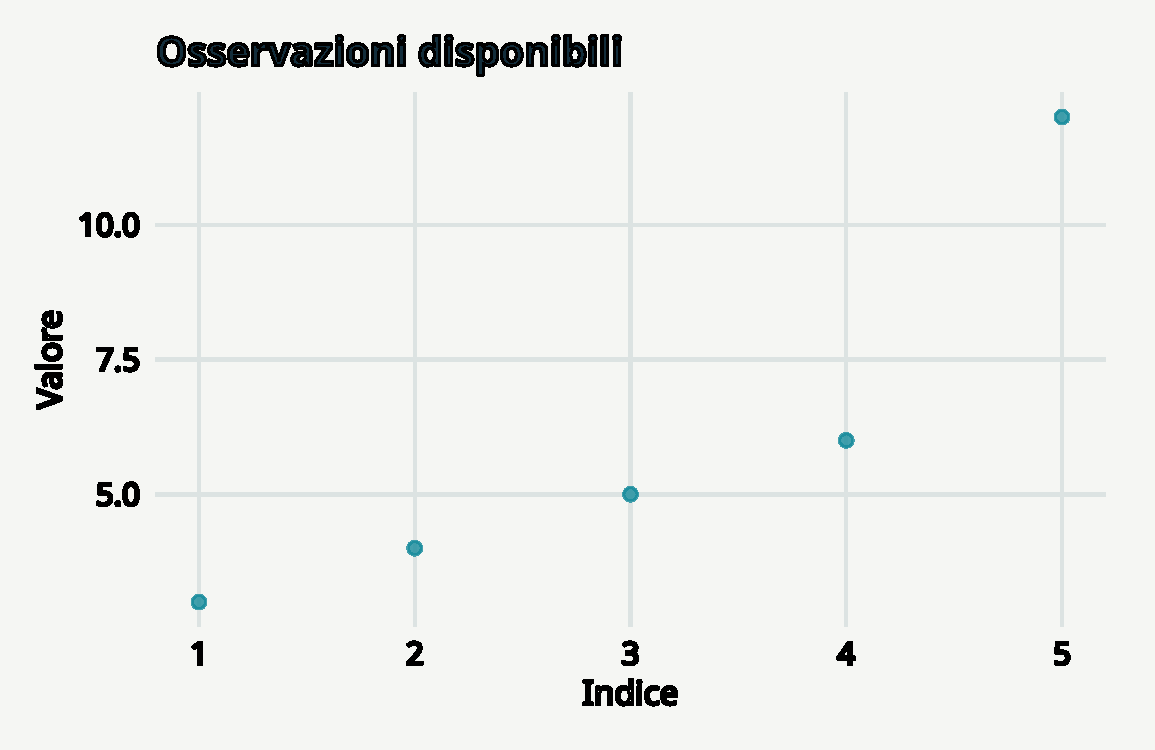
\includegraphics[width=\linewidth,height=6.0cm,keepaspectratio]{Esperimenti/t00-errori-A.pdf}\par}
\PSmall{Valore mancante: Assente. Seme: 17.}
}};
\node[anchor=north west,inner sep=0] at([xshift=10.85cm,yshift=-2.12cm]current page.north west){\Colonna{8.16cm}{\PLabel{Scenario A · simulazione}
\PBody{Il vettore comprende una misura che può essere resa indisponibile. Quando questa viene sostituita con NA, il numero delle osservazioni disponibili diminuisce e il calcolo ordinario della media restituisce un valore mancante, segnalando che il dato incompleto attraversa il procedimento.}
\par\smallskip{\centering\adjustbox{max width=.98\linewidth}{$\displaystyle n_{\rm obs}=\sum_i\mathbf{1}(x_i\ne\mathrm{NA})$}\par\smallskip}
\PSmall{$n_{\rm obs}$ conta i valori disponibili; l’indicatore vale uno quando la misura è osservata. In R la verifica dei mancanti si esegue mediante is.na().}
}};
\node[anchor=north east,inner sep=0] at([xshift=17.1cm,yshift=-12.04cm]current page.north west){\fontsize{7.7}{9}\selectfont \href{https://marzione00.github.io/Lab_Geo/\#laboratorio/t00-errori}{\color{Classical}\bfseries Apri il laboratorio · t00-errori}};
\end{tikzpicture}\end{frame}

\begin{frame}[plain]\hypertarget{slide36}{}
\bookmark[level=1,page=36]{Confronto | Diagnosi di un calcolo incompleto}
\begin{tikzpicture}[remember picture,overlay]
\PilotChrome{Confronto | Diagnosi di un calcolo incompleto}{ERRORI E CONTROLLO DEL PROCEDIMENTO}{36}{L’eliminazione dei mancanti cambia l’insieme delle osservazioni utilizzate.}
\node[anchor=north west,inner sep=0] at([xshift=.96cm,yshift=-2.12cm]current page.north west){\Colonna{9.40cm}{{\centering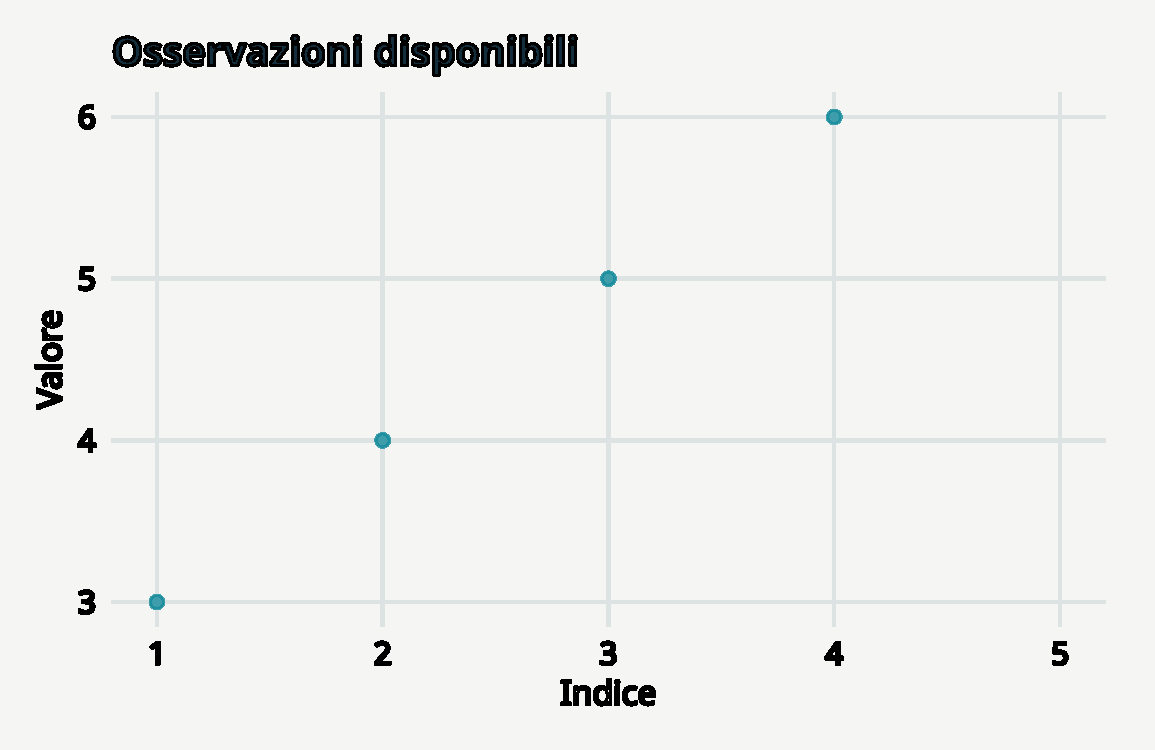
\includegraphics[width=\linewidth,height=5.6cm,keepaspectratio]{Esperimenti/t00-errori-B.pdf}\par}
\PSmall{Valore mancante: Assente $\to$ Presente. Tutti gli altri parametri e il seme sono fissi.}
}};
\node[anchor=north west,inner sep=0] at([xshift=10.85cm,yshift=-2.12cm]current page.north west){\Colonna{8.16cm}{\PLabel{Confronto fra gli scenari}
{\fontsize{10.2}{12.8}\selectfont\begin{tabular}{@{}>{\raggedright\arraybackslash}p{0.48\linewidth}@{\hspace{.13cm}}>{\raggedright\arraybackslash}p{0.224\linewidth}@{\hspace{.13cm}}>{\raggedright\arraybackslash}p{0.224\linewidth}@{}}\toprule Grandezza & A & B\\[2.3pt]
\midrule 
Osservazioni disponibili & 5 & 4\\[2.3pt]
mean(x) & 6 & NA\\[2.3pt]
mean(x, na.rm=TRUE) & 6 & 4,5\\[2.3pt]
\bottomrule\end{tabular}\par}
\vspace{.25cm}\PBody{Con il valore mancante la media diretta restituisce NA. La media dei quattro valori disponibili è 4,5 e descrive un insieme diverso.}
}};
\node[anchor=north east,inner sep=0] at([xshift=17.1cm,yshift=-12.04cm]current page.north west){\fontsize{7.7}{9}\selectfont \href{https://marzione00.github.io/Lab_Geo/\#laboratorio/t00-errori}{\color{Classical}\bfseries Apri il laboratorio · t00-errori}};
\end{tikzpicture}\end{frame}

\begin{frame}[plain]\hypertarget{slide37}{}
\bookmark[level=0,page=37]{Preparazione ed esecuzione locale}
\bookmark[level=1,page=37]{Un argomento esplicito sopravvive al riavvio}
\begin{tikzpicture}[remember picture,overlay]
\PilotChrome{Un argomento esplicito sopravvive al riavvio}{PREPARAZIONE ED ESECUZIONE LOCALE}{37}{Le quantità da cui dipende il risultato devono comparire nella procedura.}
\node[anchor=north west,inner sep=0] at([xshift=.96cm,yshift=-2.12cm]current page.north west){\Colonna{9.40cm}{\PLabel{Domanda}
\PBody{Un valore di conversione può restare nella sessione da una prova precedente. Quale informazione deve ricevere una funzione per ripartire da zero?}
\vspace{.35cm}\PLabel{Interpretazione}
\PBody{Dichiarando il fattore nella chiamata si vede subito che 2,68 g/cm³ diventano 2680 kg/m³. Una seconda esecuzione può ricostruire la conversione.}
}};
\node[anchor=north west,inner sep=0] at([xshift=10.85cm,yshift=-2.12cm]current page.north west){\Colonna{8.16cm}{\begin{tcolorbox}[enhanced,arc=1.7mm,boxrule=.6pt,colback=white,colframe=Classical!60!Navy,colbacktitle=Navy,coltitle=white,fonttitle=\bfseries\small,title={R · calcolo riproducibile},left=1.7mm,right=1.3mm,top=1.1mm,bottom=1.1mm,before skip=1mm,after skip=1.0mm]\lstinputlisting[style=GeoR,language=R]{Codice/capitolo-05.R}\end{tcolorbox}
\PLabel{Risultato in R}
\begin{tcolorbox}[colback=GeoTint,colframe=Rule,boxrule=.5pt,arc=1.4mm,left=2mm,right=1mm,top=1mm,bottom=1mm]{\fontsize{9}{12}\selectfont\ttfamily \mbox{[1]\ 2680}}\end{tcolorbox}}};
\end{tikzpicture}\end{frame}

\begin{frame}[plain]\hypertarget{slide38}{}
\bookmark[level=1,page=38]{La stessa operazione in R e Python}
\begin{tikzpicture}[remember picture,overlay]
\PilotChrome{La stessa operazione in R e Python}{PREPARAZIONE ED ESECUZIONE LOCALE}{38}{Dichiarando il fattore nella chiamata si vede subito che 2,68 g/cm³ diventano 2680 kg/m³. Una seconda esecuzione può ricostruire la conversione.}
\node[anchor=north west,inner sep=0] at([xshift=.96cm,yshift=-2.12cm]current page.north west){\Colonna{9.40cm}{\begin{tcolorbox}[enhanced,arc=1.7mm,boxrule=.6pt,colback=white,colframe=Classical!60!Navy,colbacktitle=Navy,coltitle=white,fonttitle=\bfseries\small,title={R},left=1.7mm,right=1.3mm,top=1.1mm,bottom=1.1mm,before skip=1mm,after skip=1.0mm]\lstinputlisting[style=GeoR,language=R]{Codice/capitolo-05.R}\end{tcolorbox}
\PSmall{Caso: Un argomento esplicito sopravvive al riavvio.}
}};
\node[anchor=north west,inner sep=0] at([xshift=10.85cm,yshift=-2.12cm]current page.north west){\Colonna{8.16cm}{\begin{tcolorbox}[enhanced,arc=1.7mm,boxrule=.6pt,colback=white,colframe=Classical!60!Navy,colbacktitle=Navy,coltitle=white,fonttitle=\bfseries\small,title={Python 3},left=1.7mm,right=1.3mm,top=1.1mm,bottom=1.1mm,before skip=1mm,after skip=1.0mm]\lstinputlisting[style=GeoR,language=Python]{Codice/capitolo-05.py}\end{tcolorbox}
\PInfo{Le quantità da cui dipende il risultato devono comparire nella procedura.}
}};
\end{tikzpicture}\end{frame}

\begin{frame}[plain]\hypertarget{slide39}{}
\bookmark[level=1,page=39]{Preparare runtime, interfaccia e progetto}
\begin{tikzpicture}[remember picture,overlay]
\PilotChrome{Preparare runtime, interfaccia e progetto}{PREPARAZIONE ED ESECUZIONE LOCALE}{39}{Il controllo iniziale dell’ambiente riduce l’ambiguità degli errori incontrati durante l’analisi.}
\node[anchor=north west,inner sep=0] at([xshift=.96cm,yshift=-2.12cm]current page.north west){\Colonna{9.40cm}{{\centering\resizebox{.97\linewidth}{!}{\begin{tikzpicture}[x=1cm,y=-.87cm,every node/.style={font=\fontsize{12.2}{15}\selectfont,text=Ink},arr/.style={-{Stealth[length=2mm]},line width=.8pt,draw=Classical}]\path[use as bounding box] (0,0) rectangle (7.45,6.2);
\draw[draw=Classical,fill=Classical!8,rounded corners=2pt,line width=.7pt] (0.25,0.25) rectangle (7.15,1.6);
\node[anchor=center,text=Classical,font=\fontsize{12}{15}\selectfont,text width=6.5cm,align=center] at (3.7,0.61) {\textbf{Ambiente}};
\node[anchor=center,text=Ink,font=\fontsize{11.3}{15}\selectfont,text width=6.5cm,align=center] at (3.7,1.2) {R e pacchetti disponibili};
\draw[arr,draw=Classical] (3.7,1.65)--(3.7,1.97);
\draw[draw=Quantum,fill=Quantum!8,rounded corners=2pt,line width=.7pt] (0.25,2.1) rectangle (7.15,3.45);
\node[anchor=center,text=Quantum,font=\fontsize{12}{15}\selectfont,text width=6.5cm,align=center] at (3.7,2.46) {\textbf{Progetto}};
\node[anchor=center,text=Ink,font=\fontsize{11.3}{15}\selectfont,text width=6.5cm,align=center] at (3.7,3.05) {Dati e codice nella cartella completa};
\draw[arr,draw=Quantum] (3.7,3.5)--(3.7,3.8200000000000003);
\draw[draw=Classical,fill=Classical!8,rounded corners=2pt,line width=.7pt] (0.25,3.95) rectangle (7.15,5.300000000000001);
\node[anchor=center,text=Classical,font=\fontsize{12}{15}\selectfont,text width=6.5cm,align=center] at (3.7,4.3100000000000005) {\textbf{Verifica}};
\node[anchor=center,text=Ink,font=\fontsize{11.3}{15}\selectfont,text width=6.5cm,align=center] at (3.7,4.9) {Laboratorio e controllo dell’esito};

\end{tikzpicture}}\par}
}};
\node[anchor=north west,inner sep=0] at([xshift=10.85cm,yshift=-2.12cm]current page.north west){\Colonna{8.16cm}{\PBody{L’esecuzione locale richiede un’installazione di R compatibile con il sistema operativo, i pacchetti utilizzati e una copia completa del progetto. Le distribuzioni ufficiali sono disponibili attraverso CRAN, con istruzioni specifiche per Windows, macOS e Linux. RStudio può essere aggiunto come interfaccia di lavoro. Dopo l’estrazione dell’archivio si apre il progetto dalla cartella principale e si verifica la lettura del primo CSV, così da separare i problemi dell’ambiente da quelli introdotti successivamente dall’analisi.}
}};
\end{tikzpicture}\end{frame}

\begin{frame}[plain]\hypertarget{slide40}{}
\bookmark[level=1,page=40]{Avviare un file e controllarne l’esito}
\begin{tikzpicture}[remember picture,overlay]
\PilotChrome{Avviare un file e controllarne l’esito}{PREPARAZIONE ED ESECUZIONE LOCALE}{40}{L’istruzione di avvio deve dichiarare cartella iniziale, file da eseguire e risultato da controllare.}
\node[anchor=north west,inner sep=0] at([xshift=.96cm,yshift=-2.12cm]current page.north west){\Colonna{9.40cm}{\PLabel{Metodo}
\PBody{Dalla radice del progetto, un terminale può eseguire il primo laboratorio mediante Rscript laboratori/T00/T00\_N01.R. Nell’ambiente di sviluppo si apre il medesimo file e lo si esegue dall’inizio, verificando messaggi e risultati. Il percorso Python usa python laboratori\_python/T00/T00\_N01.py, con un interprete nel quale siano disponibili le dipendenze dichiarate. L’esito comprende codice di terminazione, output prodotto e controlli superati; la semplice comparsa di un grafico non garantisce che tutte le istruzioni siano state completate.}
}};
\node[anchor=north west,inner sep=0] at([xshift=10.85cm,yshift=-2.12cm]current page.north west){\Colonna{8.16cm}{\PLabel{Interpretazione}
\PBody{Prima dell’esecuzione, getwd() mostra la cartella corrente in R. Il progetto include dati, funzioni di supporto, script e destinazioni dei risultati. Il trasferimento di un solo file può interrompere queste dipendenze, anche quando il codice rimane leggibile.}
}};
\end{tikzpicture}\end{frame}

\begin{frame}[plain]\hypertarget{slide41}{}
\bookmark[level=1,page=41]{Installazione, caricamento e ambiente attivo}
\begin{tikzpicture}[remember picture,overlay]
\PilotChrome{Installazione, caricamento e ambiente attivo}{PREPARAZIONE ED ESECUZIONE LOCALE}{41}{La disponibilità di un pacchetto va verificata nell’ambiente che esegue effettivamente il codice.}
\node[anchor=north west,inner sep=0] at([xshift=.96cm,yshift=-2.12cm]current page.north west){\Colonna{9.40cm}{\PLabel{Metodo}
\PBody{L’installazione rende un pacchetto disponibile in una libreria, mentre il caricamento lo rende utilizzabile nella sessione secondo le convenzioni del linguaggio. In R, library carica un pacchetto già presente; la forma pacchetto::funzione richiama esplicitamente una funzione esportata. In Python, l’ambiente virtuale separa le dipendenze del progetto e viene creato dall’interprete selezionato. Quando un pacchetto risulta installato ma non viene trovato, si confrontano ambiente attivo, percorsi delle librerie e processo utilizzato dall’interfaccia.}
}};
\node[anchor=north west,inner sep=0] at([xshift=10.85cm,yshift=-2.12cm]current page.north west){\Colonna{8.16cm}{\PLabel{Interpretazione}
\PBody{La preparazione delle dipendenze precede gli script analitici. Per Python, python -m venv .venv crea un ambiente dall’interprete richiamato; python -m pip collega l’installazione a quell’interprete. In R, sessionInfo() e .libPaths() documentano ambiente e librerie utilizzate.}
}};
\end{tikzpicture}\end{frame}

\begin{frame}[plain]\hypertarget{slide42}{}
\bookmark[level=1,page=42]{Notebook, ordine delle celle e stato della sessione}
\begin{tikzpicture}[remember picture,overlay]
\PilotChrome{Notebook, ordine delle celle e stato della sessione}{PREPARAZIONE ED ESECUZIONE LOCALE}{42}{La verifica da una sessione pulita collega il documento salvato al procedimento effettivamente eseguibile.}
\node[anchor=north west,inner sep=0] at([xshift=.96cm,yshift=-2.12cm]current page.north west){\Colonna{9.40cm}{{\centering\resizebox{.97\linewidth}{!}{\begin{tikzpicture}[x=1cm,y=-.87cm,every node/.style={font=\fontsize{12.2}{15}\selectfont,text=Ink},arr/.style={-{Stealth[length=2mm]},line width=.8pt,draw=Classical}]\path[use as bounding box] (0,0) rectangle (7.45,6.2);
\draw[draw=Classical,fill=Classical!8,rounded corners=2pt,line width=.7pt] (0.5,0.6) rectangle (6.9,2);
\node[anchor=center,text=Ink,font=\fontsize{11.5}{15}\selectfont,text width=6.1cm,align=center] at (3.7,1.3) {Documento: testo, codice e output salvati};
\draw[arr,draw=Classical] (3.7,2.2)--(3.7,3);
\draw[draw=Quantum,fill=Quantum!8,rounded corners=2pt,line width=.7pt] (0.5,3.2) rectangle (6.9,4.6);
\node[anchor=center,text=Ink,font=\fontsize{11.5}{15}\selectfont,text width=6.1cm,align=center] at (3.7,3.9) {Kernel: oggetti e stato della sessione};
\node[anchor=center,text=Ink,font=\fontsize{11}{15}\selectfont,text width=6.8cm,align=center] at (3.7,5.6) {Riavvio ed esecuzione ordinata verificano le dipendenze.};

\end{tikzpicture}}\par}
}};
\node[anchor=north west,inner sep=0] at([xshift=10.85cm,yshift=-2.12cm]current page.north west){\Colonna{8.16cm}{\PBody{Un notebook conserva testo, codice e output, mentre il kernel mantiene gli oggetti della sessione di esecuzione. Una cella avviata fuori ordine può utilizzare valori creati in precedenza e produrre un risultato che il documento, letto dall’inizio, non ricostruisce. Il controllo consiste nel riavviare il processo ed eseguire tutte le celle in ordine, verificando dipendenze e risultati. Un output salvato nel documento testimonia una precedente esecuzione, della quale occorre distinguere il contenuto dallo stato attualmente disponibile in memoria.}
}};
\end{tikzpicture}\end{frame}

\begin{frame}[plain]\hypertarget{slide43}{}
\bookmark[level=1,page=43]{Sessione pulita e dipendenze}
\begin{tikzpicture}[remember picture,overlay]
\PilotChrome{Sessione pulita e dipendenze}{PREPARAZIONE ED ESECUZIONE LOCALE}{43}{Riconoscere un risultato che dipende da un oggetto precedente.}
\node[anchor=north west,inner sep=0] at([xshift=.96cm,yshift=-2.12cm]current page.north west){\Colonna{9.40cm}{{\centering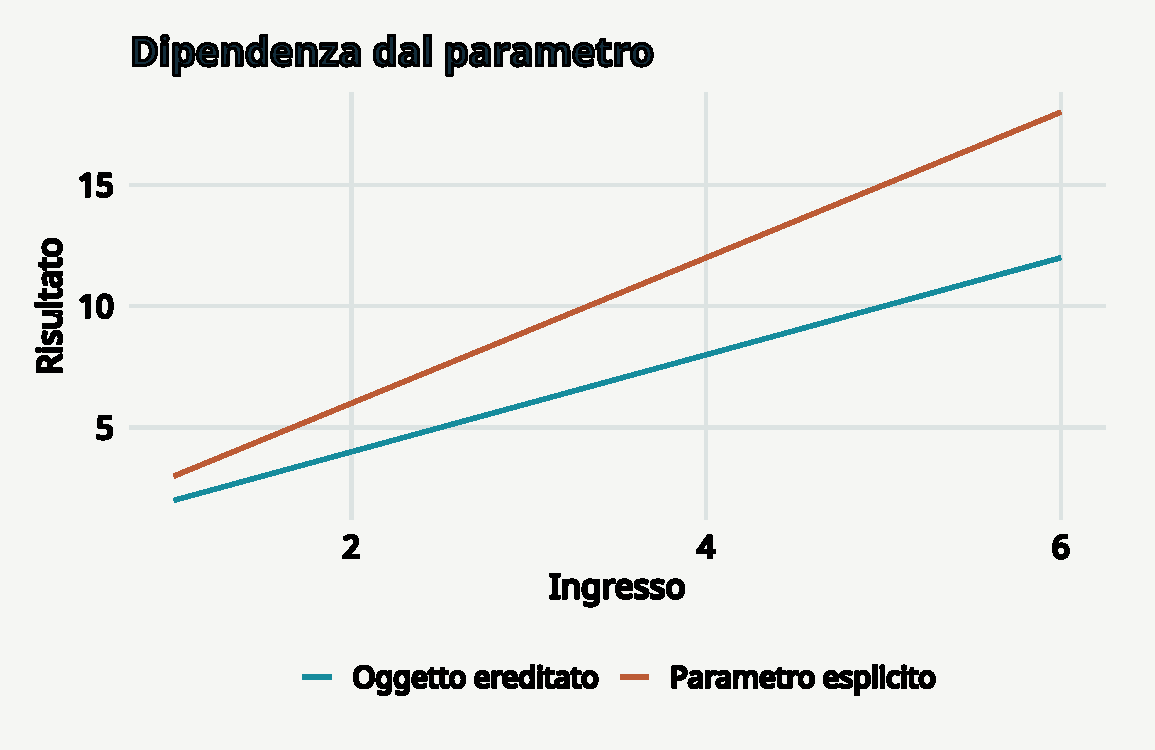
\includegraphics[width=\linewidth,height=6.0cm,keepaspectratio]{Esperimenti/t00-sessione-A.pdf}\par}
\PSmall{Fattore ereditato dalla sessione: 2. Seme: 17.}
}};
\node[anchor=north west,inner sep=0] at([xshift=10.85cm,yshift=-2.12cm]current page.north west){\Colonna{8.16cm}{\PLabel{Scenario A · simulazione}
\PBody{Due procedimenti applicano allo stesso vettore fattori di moltiplicazione differenti. Uno rappresenta il valore che potrebbe essere ereditato da una sessione precedente; l’altro utilizza un parametro dichiarato. Entrambi sono resi visibili nel pannello, così da poter attribuire lo scarto dei risultati a una dipendenza precisa.}
\par\smallskip{\centering\adjustbox{max width=.98\linewidth}{$\displaystyle y=f(x;\theta)$}\par\smallskip}
\PSmall{$x$ rappresenta i dati d’ingresso; $\theta$ indica il parametro della procedura; $f$ è la trasformazione applicata; $y$ è il risultato.}
}};
\node[anchor=north east,inner sep=0] at([xshift=17.1cm,yshift=-12.04cm]current page.north west){\fontsize{7.7}{9}\selectfont \href{https://marzione00.github.io/Lab_Geo/\#laboratorio/t00-sessione}{\color{Classical}\bfseries Apri il laboratorio · t00-sessione}};
\end{tikzpicture}\end{frame}

\begin{frame}[plain]\hypertarget{slide44}{}
\bookmark[level=1,page=44]{Confronto | Sessione pulita e dipendenze}
\begin{tikzpicture}[remember picture,overlay]
\PilotChrome{Confronto | Sessione pulita e dipendenze}{PREPARAZIONE ED ESECUZIONE LOCALE}{44}{Il risultato riproducibile dipende da dati e parametri dichiarati.}
\node[anchor=north west,inner sep=0] at([xshift=.96cm,yshift=-2.12cm]current page.north west){\Colonna{9.40cm}{{\centering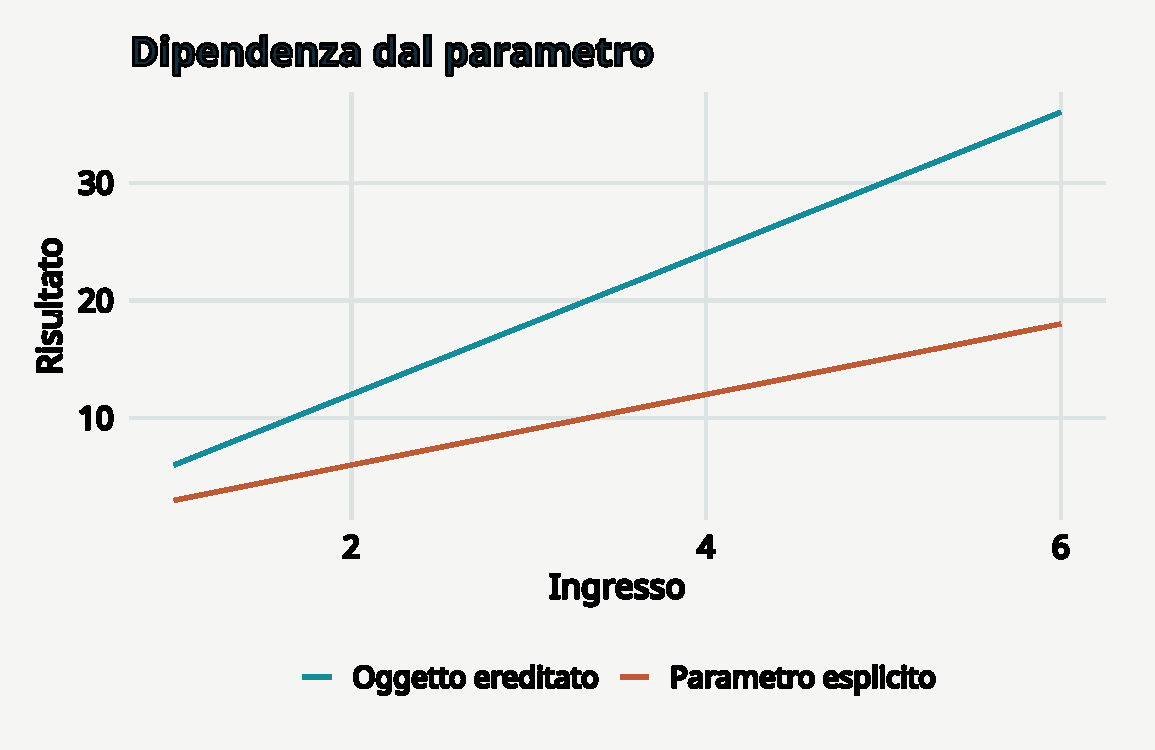
\includegraphics[width=\linewidth,height=5.6cm,keepaspectratio]{Esperimenti/t00-sessione-B.pdf}\par}
\PSmall{Fattore ereditato dalla sessione: 2 $\to$ 6. Tutti gli altri parametri e il seme sono fissi.}
}};
\node[anchor=north west,inner sep=0] at([xshift=10.85cm,yshift=-2.12cm]current page.north west){\Colonna{8.16cm}{\PLabel{Confronto fra gli scenari}
{\fontsize{10.2}{12.8}\selectfont\begin{tabular}{@{}>{\raggedright\arraybackslash}p{0.48\linewidth}@{\hspace{.13cm}}>{\raggedright\arraybackslash}p{0.224\linewidth}@{\hspace{.13cm}}>{\raggedright\arraybackslash}p{0.224\linewidth}@{}}\toprule Grandezza & A & B\\[2.3pt]
\midrule 
Scarto massimo & 6 & 18\\[2.3pt]
\bottomrule\end{tabular}\par}
\vspace{.25cm}\PBody{Portando a 6 il fattore ereditato, la distanza fra le due procedure cresce. La funzione con argomento esplicito usa ancora 3.}
}};
\node[anchor=north east,inner sep=0] at([xshift=17.1cm,yshift=-12.04cm]current page.north west){\fontsize{7.7}{9}\selectfont \href{https://marzione00.github.io/Lab_Geo/\#laboratorio/t00-sessione}{\color{Classical}\bfseries Apri il laboratorio · t00-sessione}};
\end{tikzpicture}\end{frame}

\begin{frame}[plain]\hypertarget{slide45}{}
\bookmark[level=0,page=45]{Scelte di strumenti e prestazioni}
\bookmark[level=1,page=45]{Il divisore decide la dispersione}
\begin{tikzpicture}[remember picture,overlay]
\PilotChrome{Il divisore decide la dispersione}{SCELTE DI STRUMENTI E PRESTAZIONI}{45}{Annota il divisore quando confronti funzioni statistiche.}
\node[anchor=north west,inner sep=0] at([xshift=.96cm,yshift=-2.12cm]current page.north west){\Colonna{9.40cm}{\PLabel{Domanda}
\PBody{R e Python ricevono gli stessi tre numeri. Quale definizione di deviazione standard permette un confronto ripetibile?}
\vspace{.35cm}\PLabel{Interpretazione}
\PBody{Con divisore 2 la deviazione standard vale 1. Con divisore 3 vale circa 0,8165. Entrambe le espressioni usano scarti rispetto alla media.}
}};
\node[anchor=north west,inner sep=0] at([xshift=10.85cm,yshift=-2.12cm]current page.north west){\Colonna{8.16cm}{\begin{tcolorbox}[enhanced,arc=1.7mm,boxrule=.6pt,colback=white,colframe=Classical!60!Navy,colbacktitle=Navy,coltitle=white,fonttitle=\bfseries\small,title={R · calcolo riproducibile},left=1.7mm,right=1.3mm,top=1.1mm,bottom=1.1mm,before skip=1mm,after skip=1.0mm]\lstinputlisting[style=GeoR,language=R]{Codice/capitolo-06.R}\end{tcolorbox}
\PLabel{Risultato in R}
\begin{tcolorbox}[colback=GeoTint,colframe=Rule,boxrule=.5pt,arc=1.4mm,left=2mm,right=1mm,top=1mm,bottom=1mm]{\fontsize{9}{12}\selectfont\ttfamily \mbox{campione\ popolazione\ }\\\mbox{\ \ 1.0000000\ \ \ 0.8164966}}\end{tcolorbox}}};
\end{tikzpicture}\end{frame}

\begin{frame}[plain]\hypertarget{slide46}{}
\bookmark[level=1,page=46]{La stessa operazione in R e Python}
\begin{tikzpicture}[remember picture,overlay]
\PilotChrome{La stessa operazione in R e Python}{SCELTE DI STRUMENTI E PRESTAZIONI}{46}{Con divisore 2 la deviazione standard vale 1. Con divisore 3 vale circa 0,8165. Entrambe le espressioni usano scarti rispetto alla media.}
\node[anchor=north west,inner sep=0] at([xshift=.96cm,yshift=-2.12cm]current page.north west){\Colonna{9.40cm}{\begin{tcolorbox}[enhanced,arc=1.7mm,boxrule=.6pt,colback=white,colframe=Classical!60!Navy,colbacktitle=Navy,coltitle=white,fonttitle=\bfseries\small,title={R},left=1.7mm,right=1.3mm,top=1.1mm,bottom=1.1mm,before skip=1mm,after skip=1.0mm]\lstinputlisting[style=GeoR,language=R]{Codice/capitolo-06.R}\end{tcolorbox}
\PSmall{Caso: Il divisore decide la dispersione.}
}};
\node[anchor=north west,inner sep=0] at([xshift=10.85cm,yshift=-2.12cm]current page.north west){\Colonna{8.16cm}{\begin{tcolorbox}[enhanced,arc=1.7mm,boxrule=.6pt,colback=white,colframe=Classical!60!Navy,colbacktitle=Navy,coltitle=white,fonttitle=\bfseries\small,title={Python 3},left=1.7mm,right=1.3mm,top=1.1mm,bottom=1.1mm,before skip=1mm,after skip=1.0mm]\lstinputlisting[style=GeoR,language=Python]{Codice/capitolo-06.py}\end{tcolorbox}
\PInfo{Annota il divisore quando confronti funzioni statistiche.}
}};
\end{tikzpicture}\end{frame}

\begin{frame}[plain]\hypertarget{slide47}{}
\bookmark[level=1,page=47]{Convenzioni statistiche e confronto fra linguaggi}
\begin{tikzpicture}[remember picture,overlay]
\PilotChrome{Convenzioni statistiche e confronto fra linguaggi}{SCELTE DI STRUMENTI E PRESTAZIONI}{47}{L’equivalenza metodologica richiede convenzioni esplicite oltre alla corrispondenza della sintassi.}
\node[anchor=north west,inner sep=0] at([xshift=.96cm,yshift=-2.12cm]current page.north west){\Colonna{9.40cm}{{\centering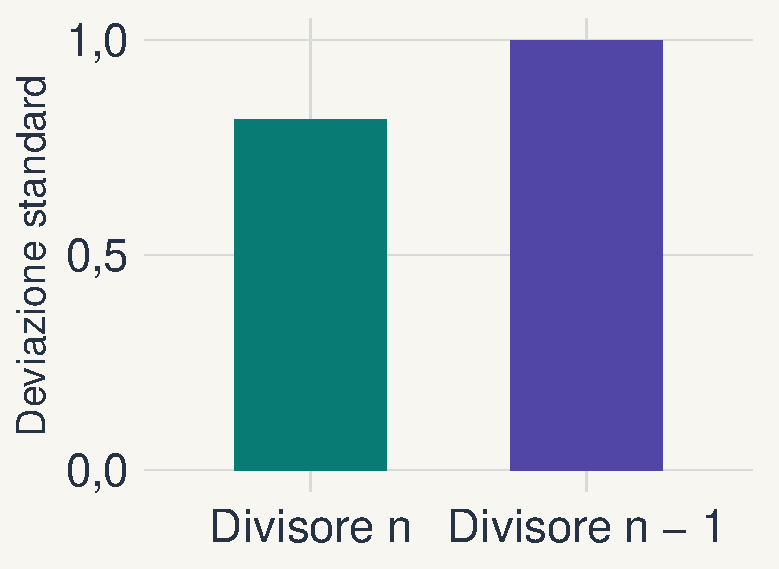
\includegraphics[width=\linewidth,height=6.15cm,keepaspectratio]{Figure/F04.pdf}\par}
\PSmall{Deviazioni standard dei valori 1, 2, 3 secondo due divisori. Il confronto usa gli stessi dati.}
}};
\node[anchor=north west,inner sep=0] at([xshift=10.85cm,yshift=-2.12cm]current page.north west){\Colonna{8.16cm}{\PBody{Due implementazioni possono restituire risultati differenti perché adottano convenzioni diverse, pur applicando entrambe formule corrette. Per i tre valori $x_i$ = 1, 2, 3, con n = 3 e media pari a 2, la deviazione standard con divisore n vale circa 0,8165, mentre quella con divisore n meno uno vale uno. R sd usa il secondo criterio; NumPy richiede ddof uguale a uno per ottenere lo stesso risultato. Il confronto deve perciò dichiarare formula, gestione dei mancanti, ordine delle righe e parametri, prima di attribuire una differenza al linguaggio.}
\par\smallskip{\centering\adjustbox{max width=.98\linewidth}{$\displaystyle s=\sqrt{\frac{\sum_i(x_i-\overline x)^2}{n-1}},\qquad\sigma_n=\sqrt{\frac{\sum_i(x_i-\overline x)^2}{n}}$}\par\smallskip}
}};
\end{tikzpicture}\end{frame}

\begin{frame}[plain]\hypertarget{slide48}{}
\bookmark[level=1,page=48]{Ecosistemi e criteri di scelta}
\begin{tikzpicture}[remember picture,overlay]
\PilotChrome{Ecosistemi e criteri di scelta}{SCELTE DI STRUMENTI E PRESTAZIONI}{48}{Lo strumento viene scelto rispetto al compito, alle dipendenze e alle competenze disponibili.}
\node[anchor=north west,inner sep=0] at([xshift=.96cm,yshift=-2.12cm]current page.north west){\Colonna{9.40cm}{\PLabel{Metodo}
\PBody{R offre un ambiente dedicato al calcolo statistico, nel quale formule dei modelli e rappresentazioni grafiche costituiscono elementi centrali del lavoro. Python collega analisi numerica e attività generaliste attraverso librerie e strumenti differenti. La scelta per un progetto dipende da competenze del gruppo, metodi necessari, integrazione con altri sistemi e manutenzione del codice. Nel corso, R mantiene continuità con le lezioni statistiche, mentre il confronto Python serve a distinguere le scelte analitiche dalle convenzioni delle librerie utilizzate.}
}};
\node[anchor=north west,inner sep=0] at([xshift=10.85cm,yshift=-2.12cm]current page.north west){\Colonna{8.16cm}{\PLabel{Interpretazione}
\PBody{Il riciclo dei vettori, la selezione delle colonne, la gestione degli indici e i valori predefiniti richiedono attenzione in entrambi gli ecosistemi. La documentazione della funzione utilizzata e un esempio verificabile offrono un riferimento più utile di una graduatoria generale fra linguaggi.}
}};
\end{tikzpicture}\end{frame}

\begin{frame}[plain]\hypertarget{slide49}{}
\bookmark[level=1,page=49]{Costo dell’algoritmo e dimensione del problema}
\begin{tikzpicture}[remember picture,overlay]
\PilotChrome{Costo dell’algoritmo e dimensione del problema}{SCELTE DI STRUMENTI E PRESTAZIONI}{49}{La prestazione computazionale deve essere misurata su un compito definito e con risultati equivalenti.}
\node[anchor=north west,inner sep=0] at([xshift=.96cm,yshift=-2.12cm]current page.north west){\Colonna{9.40cm}{{\centering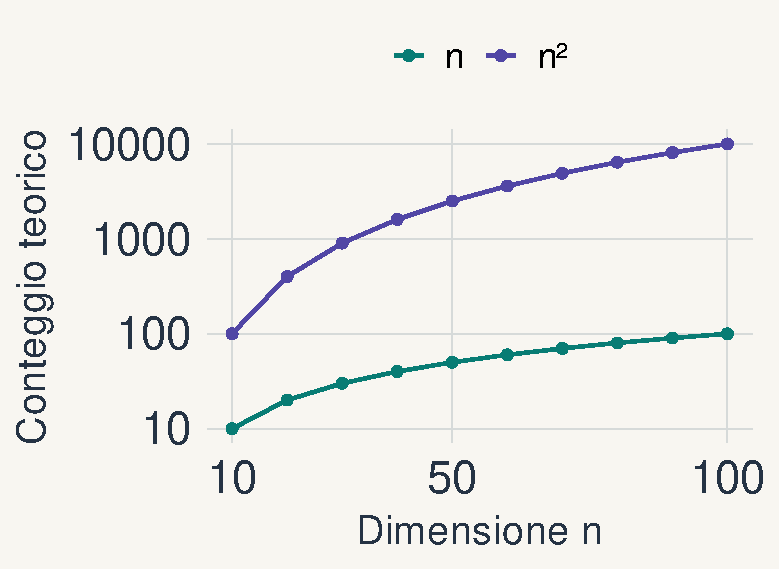
\includegraphics[width=\linewidth,height=6.15cm,keepaspectratio]{Figure/F05.pdf}\par}
\PSmall{Conteggi teorici n e n² su asse verticale logaritmico. La figura illustra la crescita, senza costituire un benchmark.}
}};
\node[anchor=north west,inner sep=0] at([xshift=10.85cm,yshift=-2.12cm]current page.north west){\Colonna{8.16cm}{\PBody{Il tempo di esecuzione dipende da algoritmo, dimensione dei dati, librerie native, memoria e organizzazione del calcolo. La figura confronta due conteggi teorici, proporzionali a n e a n al quadrato, per mostrare come un aumento della dimensione possa amplificare differenze algoritmiche. I valori rappresentano operazioni ipotetiche e non tempi misurati. Un confronto fra implementazioni richiede lo stesso compito, dati equivalenti, risultati verificati e misure ripetute, separando eventuali costi di caricamento o inizializzazione.}
}};
\end{tikzpicture}\end{frame}

\begin{frame}[plain]\hypertarget{slide50}{}
\bookmark[level=1,page=50]{Memoria, parallelismo e trasferimenti}
\begin{tikzpicture}[remember picture,overlay]
\PilotChrome{Memoria, parallelismo e trasferimenti}{SCELTE DI STRUMENTI E PRESTAZIONI}{50}{Risorse e parallelismo vanno valutati rispetto alla struttura delle operazioni e dei dati.}
\node[anchor=north west,inner sep=0] at([xshift=.96cm,yshift=-2.12cm]current page.north west){\Colonna{9.40cm}{\PLabel{Metodo}
\PBody{Una matrice densa con n righe e p colonne di numeri a doppia precisione richiede circa otto byte per elemento, ai quali si aggiungono struttura dell’oggetto e copie temporanee. Operazioni che creano matrici intermedie possono quindi richiedere più memoria del solo input. Il calcolo parallelo distribuisce parti del lavoro, introducendo costi di coordinamento e trasferimento. Un processore grafico (GPU) accelera compiti per i quali esistano implementazioni appropriate e una quantità di lavoro sufficiente; la sua presenza non modifica automaticamente il codice eseguito sul processore centrale (CPU).}
}};
\node[anchor=north west,inner sep=0] at([xshift=10.85cm,yshift=-2.12cm]current page.north west){\Colonna{8.16cm}{\PLabel{Formalismo}
\par\smallskip{\centering\adjustbox{max width=.98\linewidth}{$\displaystyle M_{valori}\simeq8np\ \mathrm{byte}\quad\text{per una matrice double }n\times p$}\par\smallskip}
\PLabel{Interpretazione}
\PBody{La misura della memoria deve includere gli oggetti intermedi effettivamente creati. Per ridurre i costi può essere più efficace cambiare rappresentazione, evitare copie o riformulare l’algoritmo, prima di distribuire il lavoro su più processi.}
}};
\end{tikzpicture}\end{frame}

\begin{frame}[plain]\hypertarget{slide51}{}
\bookmark[level=1,page=51]{Ciclo e calcolo vettoriale}
\begin{tikzpicture}[remember picture,overlay]
\PilotChrome{Ciclo e calcolo vettoriale}{SCELTE DI STRUMENTI E PRESTAZIONI}{51}{Verificare l’equivalenza numerica di due procedimenti.}
\node[anchor=north west,inner sep=0] at([xshift=.96cm,yshift=-2.12cm]current page.north west){\Colonna{9.40cm}{{\centering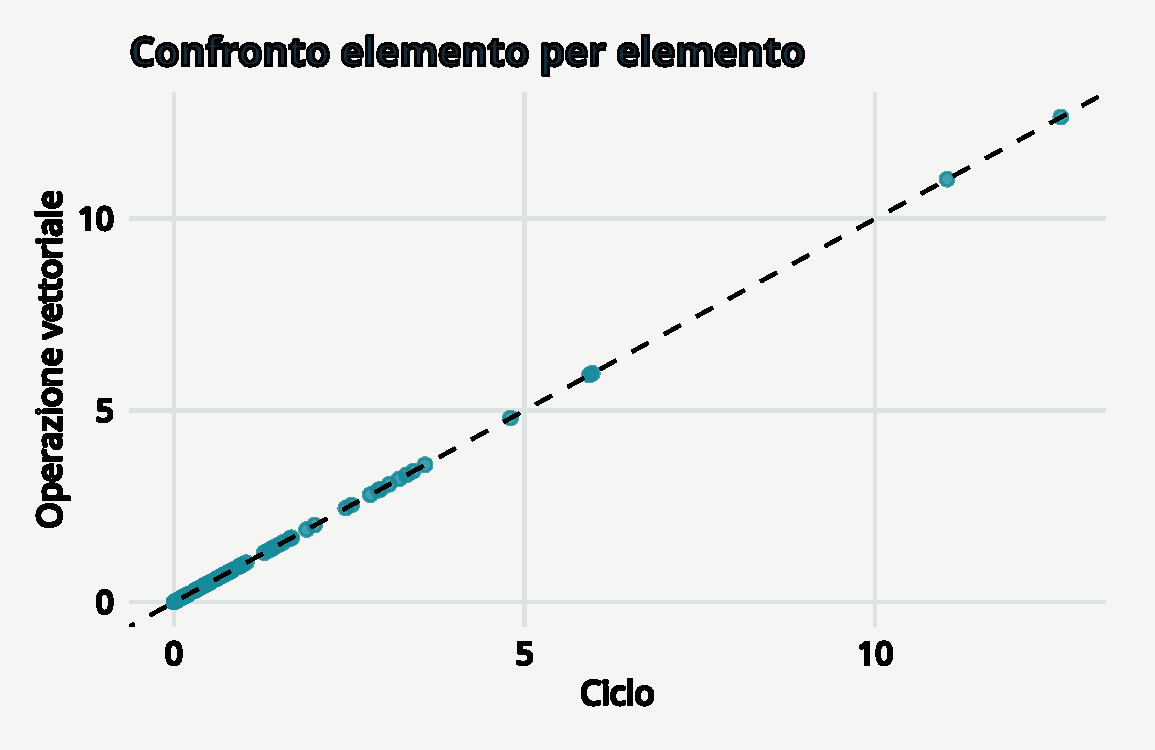
\includegraphics[width=\linewidth,height=6.0cm,keepaspectratio]{Esperimenti/t00-prestazioni-A.pdf}\par}
\PSmall{Lunghezza del vettore: 100. Seme: 17.}
}};
\node[anchor=north west,inner sep=0] at([xshift=10.85cm,yshift=-2.12cm]current page.north west){\Colonna{8.16cm}{\PLabel{Scenario A · simulazione}
\PBody{Il vettore simulato viene elevato al quadrato mediante due procedimenti: un ciclo che visita gli elementi in successione e un’operazione vettoriale che esprime direttamente la trasformazione dell’intero oggetto. Ogni punto del grafico confronta i risultati ottenuti per il medesimo elemento.}
\par\smallskip{\centering\adjustbox{max width=.98\linewidth}{$\displaystyle \sum_{i=1}^n x_i^2=\lVert x\rVert^2$}\par\smallskip}
\PSmall{$x_i$ è l’elemento $i$ del vettore di lunghezza $n$; $\lVert x\rVert^2$ è la somma dei quadrati degli elementi.}
}};
\node[anchor=north east,inner sep=0] at([xshift=17.1cm,yshift=-12.04cm]current page.north west){\fontsize{7.7}{9}\selectfont \href{https://marzione00.github.io/Lab_Geo/\#laboratorio/t00-prestazioni}{\color{Classical}\bfseries Apri il laboratorio · t00-prestazioni}};
\end{tikzpicture}\end{frame}

\begin{frame}[plain]\hypertarget{slide52}{}
\bookmark[level=1,page=52]{Confronto | Ciclo e calcolo vettoriale}
\begin{tikzpicture}[remember picture,overlay]
\PilotChrome{Confronto | Ciclo e calcolo vettoriale}{SCELTE DI STRUMENTI E PRESTAZIONI}{52}{L’equivalenza dei valori precede il confronto delle prestazioni, che dipendono dall’ambiente.}
\node[anchor=north west,inner sep=0] at([xshift=.96cm,yshift=-2.12cm]current page.north west){\Colonna{9.40cm}{{\centering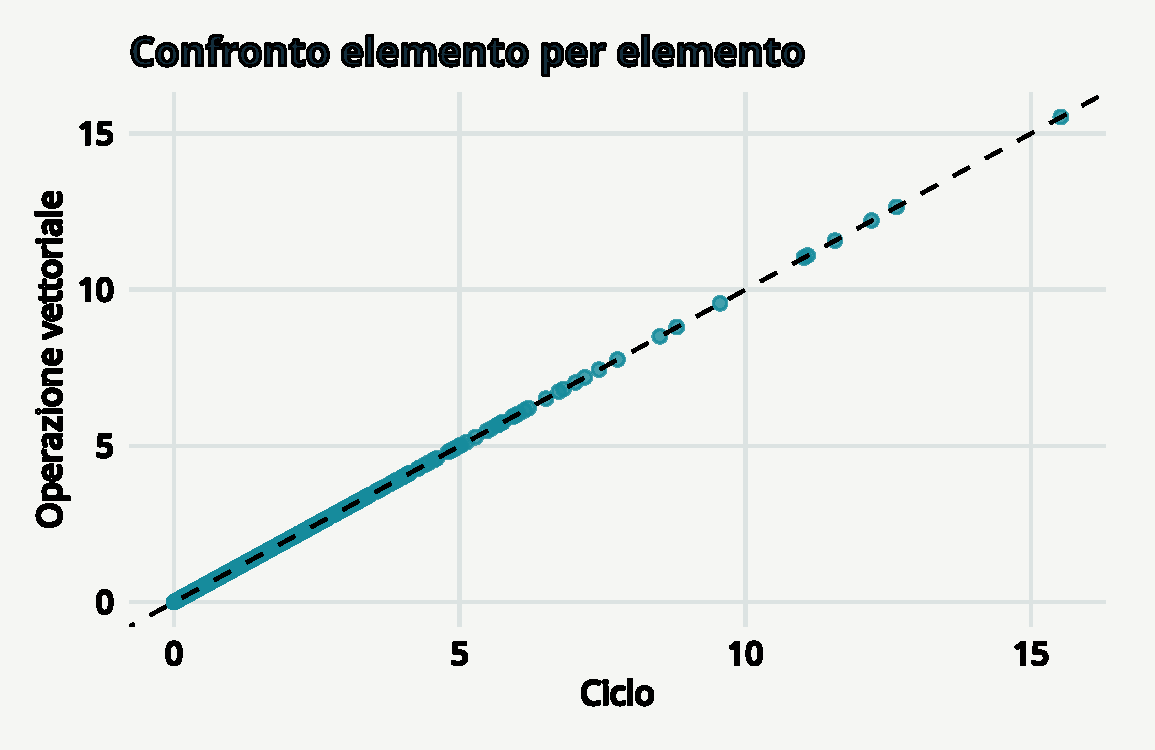
\includegraphics[width=\linewidth,height=5.6cm,keepaspectratio]{Esperimenti/t00-prestazioni-B.pdf}\par}
\PSmall{Lunghezza del vettore: 100 $\to$ 1000. Tutti gli altri parametri e il seme sono fissi.}
}};
\node[anchor=north west,inner sep=0] at([xshift=10.85cm,yshift=-2.12cm]current page.north west){\Colonna{8.16cm}{\PLabel{Confronto fra gli scenari}
{\fontsize{10.2}{12.8}\selectfont\begin{tabular}{@{}>{\raggedright\arraybackslash}p{0.48\linewidth}@{\hspace{.13cm}}>{\raggedright\arraybackslash}p{0.224\linewidth}@{\hspace{.13cm}}>{\raggedright\arraybackslash}p{0.224\linewidth}@{}}\toprule Grandezza & A & B\\[2.3pt]
\midrule 
Scarto massimo & 0 & 0\\[2.3pt]
Elementi verificati & 100 & 1000\\[2.3pt]
\bottomrule\end{tabular}\par}
\vspace{.25cm}\PBody{Passando da 100 a 1000 elementi, lo scarto numerico fra i due metodi rimane zero. Questo controllo stabilisce equivalenza sui dati provati, senza misurare i tempi.}
}};
\node[anchor=north east,inner sep=0] at([xshift=17.1cm,yshift=-12.04cm]current page.north west){\fontsize{7.7}{9}\selectfont \href{https://marzione00.github.io/Lab_Geo/\#laboratorio/t00-prestazioni}{\color{Classical}\bfseries Apri il laboratorio · t00-prestazioni}};
\end{tikzpicture}\end{frame}

\begin{frame}[plain]\hypertarget{slide53}{}
\bookmark[level=0,page=53]{Esecuzione remota e persistenza}
\bookmark[level=1,page=53]{Che cosa sopravvive alla chiusura?}
\begin{tikzpicture}[remember picture,overlay]
\PilotChrome{Che cosa sopravvive alla chiusura?}{ESECUZIONE REMOTA E PERSISTENZA}{53}{Il file esportato va verificato dal punto di vista di chi lo riapre.}
\node[anchor=north west,inner sep=0] at([xshift=.96cm,yshift=-2.12cm]current page.north west){\Colonna{9.40cm}{\PLabel{Domanda}
\PBody{La tabella è in memoria, la sessione sta per terminare. Quale controllo conferma che l’esportazione conserva le tre misure?}
\vspace{.35cm}\PLabel{Interpretazione}
\PBody{Rileggete il file in un nuovo oggetto. Confrontate identificativi e valori. Contare le righe da solo lascerebbe passare uno scambio fra due campioni.}
}};
\node[anchor=north west,inner sep=0] at([xshift=10.85cm,yshift=-2.12cm]current page.north west){\Colonna{8.16cm}{\begin{tcolorbox}[enhanced,arc=1.7mm,boxrule=.6pt,colback=white,colframe=Classical!60!Navy,colbacktitle=Navy,coltitle=white,fonttitle=\bfseries\small,title={R · calcolo riproducibile},left=1.7mm,right=1.3mm,top=1.1mm,bottom=1.1mm,before skip=1mm,after skip=1.0mm]\lstinputlisting[style=GeoR,language=R]{Codice/capitolo-07.R}\end{tcolorbox}
\PLabel{Risultato in R}
\begin{tcolorbox}[colback=GeoTint,colframe=Rule,boxrule=.5pt,arc=1.4mm,left=2mm,right=1mm,top=1mm,bottom=1mm]{\fontsize{9}{12}\selectfont\ttfamily \mbox{[1]\ TRUE}}\end{tcolorbox}}};
\end{tikzpicture}\end{frame}

\begin{frame}[plain]\hypertarget{slide54}{}
\bookmark[level=1,page=54]{Il browser può controllare un processo remoto}
\begin{tikzpicture}[remember picture,overlay]
\PilotChrome{Il browser può controllare un processo remoto}{ESECUZIONE REMOTA E PERSISTENZA}{54}{Il processo che esegue il codice determina quali risorse siano effettivamente accessibili.}
\node[anchor=north west,inner sep=0] at([xshift=.96cm,yshift=-2.12cm]current page.north west){\Colonna{9.40cm}{{\centering\resizebox{.97\linewidth}{!}{\begin{tikzpicture}[x=1cm,y=-.87cm,every node/.style={font=\fontsize{12.2}{15}\selectfont,text=Ink},arr/.style={-{Stealth[length=2mm]},line width=.8pt,draw=Classical}]\path[use as bounding box] (0,0) rectangle (7.45,6.2);
\draw[draw=Classical,fill=Classical!8,rounded corners=2pt,line width=.7pt] (0.5,0.8) rectangle (3.2,4.9);
\node[anchor=center,text=Ink,font=\fontsize{11.5}{15}\selectfont,text width=2.4cm,align=center] at (1.85,1.7) {Computer locale};
\node[anchor=center,text=Ink,font=\fontsize{12.2}{15}\selectfont,text width=2.3cm,align=center] at (1.85,3.4) {Browser};
\draw[draw=Quantum,fill=Quantum!8,rounded corners=2pt,line width=.7pt] (4.2,0.8) rectangle (6.9,4.9);
\node[anchor=center,text=Ink,font=\fontsize{11.5}{15}\selectfont,text width=2.4cm,align=center] at (5.55,1.7) {Servizio remoto};
\node[anchor=center,text=Ink,font=\fontsize{12.2}{15}\selectfont,text width=2.3cm,align=center] at (5.55,3.1) {Runtime};
\node[anchor=center,text=Ink,font=\fontsize{11}{15}\selectfont,text width=2.3cm,align=center] at (5.55,4.2) {File del progetto};
\draw[arr,draw=Classical] (3.3,3.4)--(4.1,3.4);
\node[anchor=center,text=Ink,font=\fontsize{11}{15}\selectfont,text width=6.8cm,align=center] at (3.7,5.7) {Il luogo del calcolo determina file e ambiente disponibili.};

\end{tikzpicture}}\par}
}};
\node[anchor=north west,inner sep=0] at([xshift=10.85cm,yshift=-2.12cm]current page.north west){\Colonna{8.16cm}{\PBody{Un’interfaccia aperta nel browser può comunicare con un runtime sullo stesso computer oppure con un processo ospitato da un servizio remoto. Nel secondo caso, il codice opera sui file e sulle librerie disponibili nell’ambiente remoto, che devono essere predisposti anche quando il documento è visibile localmente. La connessione collega interfaccia e processo, mentre la persistenza dei file dipende dal servizio e dalla destinazione di salvataggio. La distinzione permette di interpretare correttamente la perdita di oggetti dopo un riavvio del runtime.}
}};
\end{tikzpicture}\end{frame}

\begin{frame}[plain]\hypertarget{slide55}{}
\bookmark[level=1,page=55]{Progetti R, notebook gestiti e servizi istituzionali}
\begin{tikzpicture}[remember picture,overlay]
\PilotChrome{Progetti R, notebook gestiti e servizi istituzionali}{ESECUZIONE REMOTA E PERSISTENZA}{55}{La disponibilità dell’interfaccia va accompagnata dalla verifica dell’ambiente e delle dipendenze del progetto.}
\node[anchor=north west,inner sep=0] at([xshift=.96cm,yshift=-2.12cm]current page.north west){\Colonna{9.40cm}{\PLabel{Metodo}
\PBody{Un progetto RStudio in Posit Cloud raccoglie codice, pacchetti e dati entro un ambiente remoto; Colab offre un servizio di notebook Jupyter con runtime gestito. Un JupyterHub istituzionale dipende dalla configurazione predisposta dall’ateneo, mentre Binder costruisce ambienti dimostrativi a partire da repository configurati. Per il corso si trasferisce il progetto completo e si verifica l’ambiente prima dell’esecuzione. Risorse, durata delle sessioni e condizioni d’uso possono variare, per cui la scelta operativa si riferisce alla documentazione del servizio e al piano effettivamente disponibile.}
}};
\node[anchor=north west,inner sep=0] at([xshift=10.85cm,yshift=-2.12cm]current page.north west){\Colonna{8.16cm}{\PLabel{Interpretazione}
\PBody{Per Posit Cloud si crea un progetto RStudio, si caricano i file e si avvia il laboratorio dalla radice. Per un notebook Python si rendono disponibili anche dati e moduli di supporto, si verifica l’interprete del kernel e si esegue il documento dall’inizio.}
}};
\end{tikzpicture}\end{frame}

\begin{frame}[plain]\hypertarget{slide56}{}
\bookmark[level=1,page=56]{Recuperare i risultati prima della fine della sessione}
\begin{tikzpicture}[remember picture,overlay]
\PilotChrome{Recuperare i risultati prima della fine della sessione}{ESECUZIONE REMOTA E PERSISTENZA}{56}{La conclusione del calcolo comprende la conservazione verificata dei prodotti necessari.}
\node[anchor=north west,inner sep=0] at([xshift=.96cm,yshift=-2.12cm]current page.north west){\Colonna{9.40cm}{{\centering\resizebox{.97\linewidth}{!}{\begin{tikzpicture}[x=1cm,y=-.87cm,every node/.style={font=\fontsize{12.2}{15}\selectfont,text=Ink},arr/.style={-{Stealth[length=2mm]},line width=.8pt,draw=Classical}]\path[use as bounding box] (0,0) rectangle (7.45,6.2);
\draw[draw=Classical,fill=Classical!8,rounded corners=2pt,line width=.7pt] (0.25,0.25) rectangle (7.15,1.6);
\node[anchor=center,text=Classical,font=\fontsize{12}{15}\selectfont,text width=6.5cm,align=center] at (3.7,0.61) {\textbf{Sessione temporanea}};
\node[anchor=center,text=Ink,font=\fontsize{11.3}{15}\selectfont,text width=6.5cm,align=center] at (3.7,1.2) {Calcolo e produzione dei risultati};
\draw[arr,draw=Classical] (3.7,1.65)--(3.7,1.97);
\draw[draw=Quantum,fill=Quantum!8,rounded corners=2pt,line width=.7pt] (0.25,2.1) rectangle (7.15,3.45);
\node[anchor=center,text=Quantum,font=\fontsize{12}{15}\selectfont,text width=6.5cm,align=center] at (3.7,2.46) {\textbf{Salvataggio}};
\node[anchor=center,text=Ink,font=\fontsize{11.3}{15}\selectfont,text width=6.5cm,align=center] at (3.7,3.05) {Copia su disco persistente};
\draw[arr,draw=Quantum] (3.7,3.5)--(3.7,3.8200000000000003);
\draw[draw=Classical,fill=Classical!8,rounded corners=2pt,line width=.7pt] (0.25,3.95) rectangle (7.15,5.300000000000001);
\node[anchor=center,text=Classical,font=\fontsize{12}{15}\selectfont,text width=6.5cm,align=center] at (3.7,4.3100000000000005) {\textbf{Verifica}};
\node[anchor=center,text=Ink,font=\fontsize{11.3}{15}\selectfont,text width=6.5cm,align=center] at (3.7,4.9) {Riapertura dei file salvati};

\end{tikzpicture}}\par}
}};
\node[anchor=north west,inner sep=0] at([xshift=10.85cm,yshift=-2.12cm]current page.north west){\Colonna{8.16cm}{\PBody{Un file creato nel disco temporaneo di un runtime può essere eliminato alla cessazione della sessione, mentre il notebook salvato può conservare ancora la rappresentazione dell’output. La procedura conclude quindi l’analisi esportando tabelle e figure in una destinazione persistente e verificandone la rilettura. Il laboratorio T00\_N20 simula localmente questa situazione, copiando un risultato prima di eliminare la cartella temporanea. Nelle attività reali si controllano inoltre autorizzazioni, condizioni di utilizzo dei dati e contenuto effettivo della consegna.}
}};
\end{tikzpicture}\end{frame}

\begin{frame}[plain]\hypertarget{slide57}{}
\bookmark[level=1,page=57]{Ricostruire un risultato salvato}
\begin{tikzpicture}[remember picture,overlay]
\PilotChrome{Ricostruire un risultato salvato}{ESECUZIONE REMOTA E PERSISTENZA}{57}{Separare oggetto in memoria e dato persistente.}
\node[anchor=north west,inner sep=0] at([xshift=.96cm,yshift=-2.12cm]current page.north west){\Colonna{9.40cm}{{\centering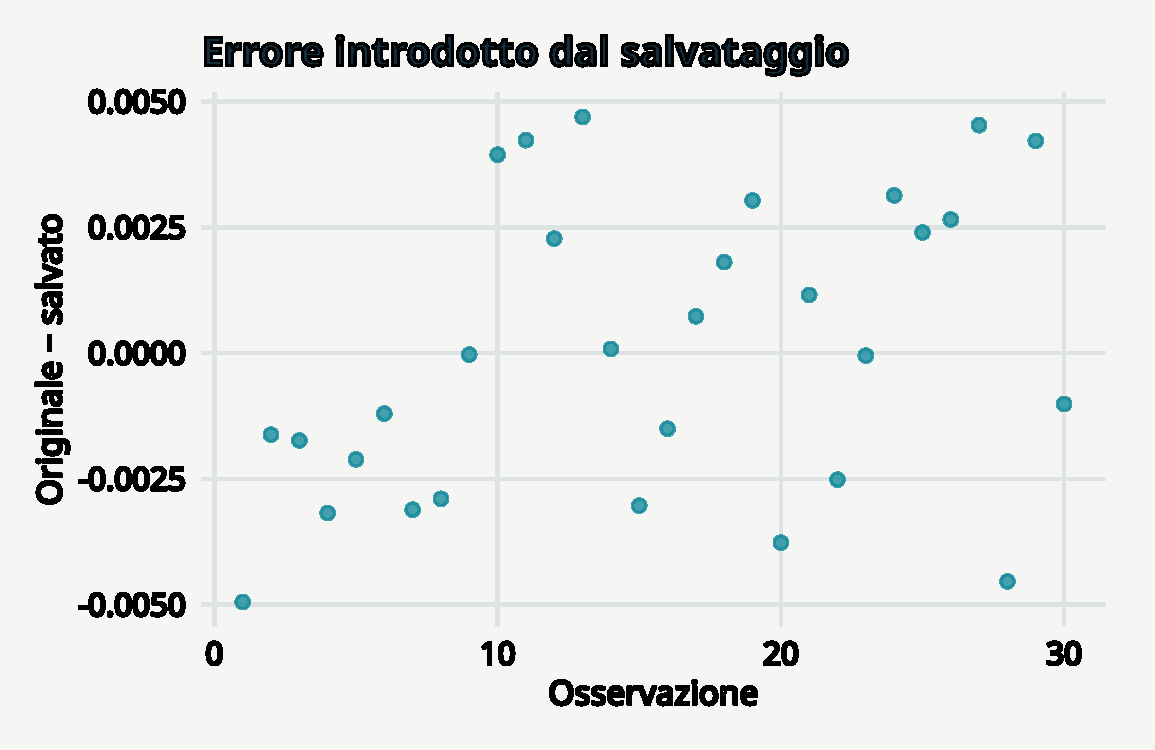
\includegraphics[width=\linewidth,height=6.0cm,keepaspectratio]{Esperimenti/t00-persistenza-A.pdf}\par}
\PSmall{Cifre decimali salvate: 2. Seme: 17.}
}};
\node[anchor=north west,inner sep=0] at([xshift=10.85cm,yshift=-2.12cm]current page.north west){\Colonna{8.16cm}{\PLabel{Scenario A · simulazione}
\PBody{Un vettore simulato viene arrotondato a un numero scelto di cifre decimali, scritto in un file CSV temporaneo e riletto in R. La differenza fra il valore recuperato e quello originario misura la perdita di precisione introdotta dall’arrotondamento, mentre il grafico permette di riconoscerne segno e ampiezza per ciascuna osservazione.}
\par\smallskip{\centering\adjustbox{max width=.98\linewidth}{$\displaystyle e_i=x_i-\operatorname{round}(x_i,d)$}\par\smallskip}
\PSmall{$d$ è il numero di cifre decimali conservate; $\operatorname{round}(x_i,d)$ è il valore arrotondato; $e_i$ è la differenza rispetto all’originale.}
}};
\node[anchor=north east,inner sep=0] at([xshift=17.1cm,yshift=-12.04cm]current page.north west){\fontsize{7.7}{9}\selectfont \href{https://marzione00.github.io/Lab_Geo/\#laboratorio/t00-persistenza}{\color{Classical}\bfseries Apri il laboratorio · t00-persistenza}};
\end{tikzpicture}\end{frame}

\begin{frame}[plain]\hypertarget{slide58}{}
\bookmark[level=1,page=58]{Confronto | Ricostruire un risultato salvato}
\begin{tikzpicture}[remember picture,overlay]
\PilotChrome{Confronto | Ricostruire un risultato salvato}{ESECUZIONE REMOTA E PERSISTENZA}{58}{La persistenza comprende formato, precisione e contesto del dato.}
\node[anchor=north west,inner sep=0] at([xshift=.96cm,yshift=-2.12cm]current page.north west){\Colonna{9.40cm}{{\centering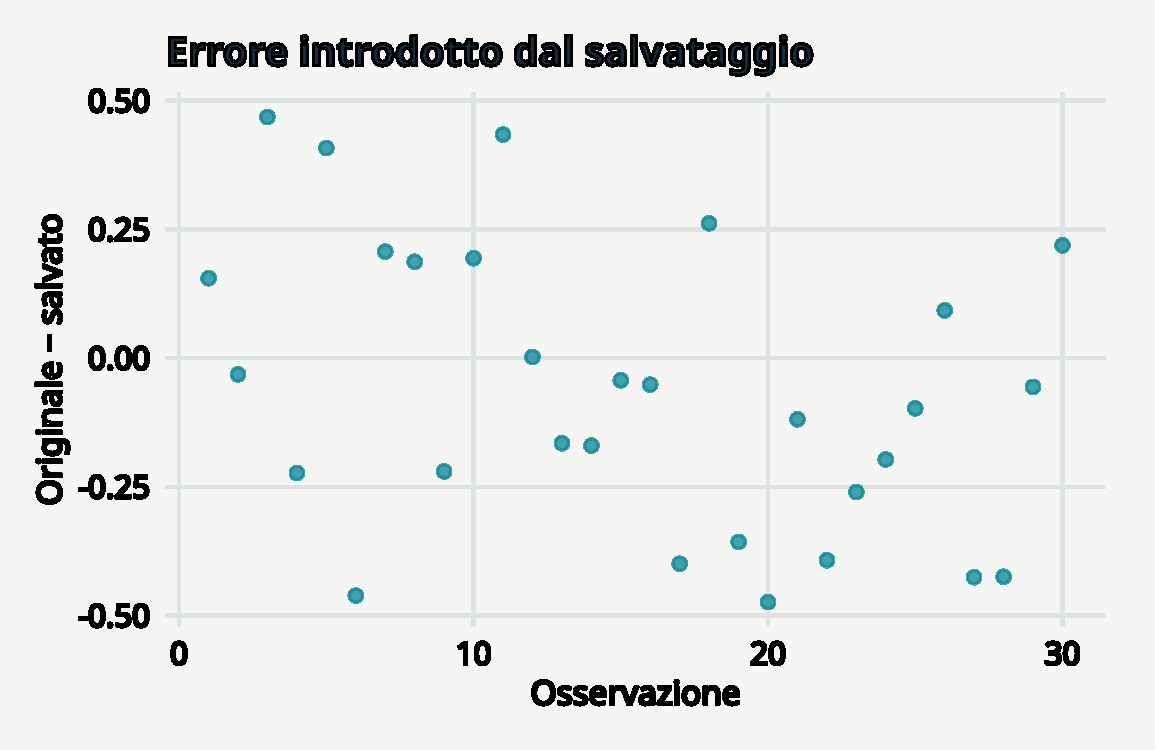
\includegraphics[width=\linewidth,height=5.6cm,keepaspectratio]{Esperimenti/t00-persistenza-B.pdf}\par}
\PSmall{Cifre decimali salvate: 2 $\to$ 0. Tutti gli altri parametri e il seme sono fissi.}
}};
\node[anchor=north west,inner sep=0] at([xshift=10.85cm,yshift=-2.12cm]current page.north west){\Colonna{8.16cm}{\PLabel{Confronto fra gli scenari}
{\fontsize{10.2}{12.8}\selectfont\begin{tabular}{@{}>{\raggedright\arraybackslash}p{0.48\linewidth}@{\hspace{.13cm}}>{\raggedright\arraybackslash}p{0.224\linewidth}@{\hspace{.13cm}}>{\raggedright\arraybackslash}p{0.224\linewidth}@{}}\toprule Grandezza & A & B\\[2.3pt]
\midrule 
Errore massimo & 0,0049492 & 0,47377\\[2.3pt]
Errore quadratico medio & 8,46e-06 & 0,079038\\[2.3pt]
\bottomrule\end{tabular}\par}
\vspace{.25cm}\PBody{Senza cifre decimali l’errore massimo supera 0,47. La perdita è già avvenuta al momento della scrittura.}
}};
\node[anchor=north east,inner sep=0] at([xshift=17.1cm,yshift=-12.04cm]current page.north west){\fontsize{7.7}{9}\selectfont \href{https://marzione00.github.io/Lab_Geo/\#laboratorio/t00-persistenza}{\color{Classical}\bfseries Apri il laboratorio · t00-persistenza}};
\end{tikzpicture}\end{frame}

\begin{frame}[plain]\hypertarget{slide59}{}
\bookmark[level=0,page=59]{Confronti e consegna del lavoro}
\bookmark[level=1,page=59]{La precisione di stampa modifica la consegna}
\begin{tikzpicture}[remember picture,overlay]
\PilotChrome{La precisione di stampa modifica la consegna}{CONFRONTI E CONSEGNA DEL LAVORO}{59}{Distingui la precisione del dato archiviato da quella mostrata al lettore.}
\node[anchor=north west,inner sep=0] at([xshift=.96cm,yshift=-2.12cm]current page.north west){\Colonna{9.40cm}{\PLabel{Domanda}
\PBody{Una densità viene esportata con una sola cifra decimale. Quanto si discosta la copia dal valore calcolato?}
\vspace{.35cm}\PLabel{Interpretazione}
\PBody{Lo scarto massimo dipende dal numero di cifre. Se il risultato viene usato in un secondo calcolo, conviene conservare più cifre nel file che nella tabella stampata.}
}};
\node[anchor=north west,inner sep=0] at([xshift=10.85cm,yshift=-2.12cm]current page.north west){\Colonna{8.16cm}{\begin{tcolorbox}[enhanced,arc=1.7mm,boxrule=.6pt,colback=white,colframe=Classical!60!Navy,colbacktitle=Navy,coltitle=white,fonttitle=\bfseries\small,title={R · calcolo riproducibile},left=1.7mm,right=1.3mm,top=1.1mm,bottom=1.1mm,before skip=1mm,after skip=1.0mm]\lstinputlisting[style=GeoR,language=R]{Codice/capitolo-08.R}\end{tcolorbox}
\PLabel{Risultato in R}
\begin{tcolorbox}[colback=GeoTint,colframe=Rule,boxrule=.5pt,arc=1.4mm,left=2mm,right=1mm,top=1mm,bottom=1mm]{\fontsize{9}{12}\selectfont\ttfamily \mbox{[1]\ 0.05}}\end{tcolorbox}}};
\end{tikzpicture}\end{frame}

\begin{frame}[plain]\hypertarget{slide60}{}
\bookmark[level=1,page=60]{Identità delle estrazioni e delle rappresentazioni}
\begin{tikzpicture}[remember picture,overlay]
\PilotChrome{Identità delle estrazioni e delle rappresentazioni}{CONFRONTI E CONSEGNA DEL LAVORO}{60}{Il criterio di equivalenza va definito rispetto alla quantità scientifica rappresentata.}
\node[anchor=north west,inner sep=0] at([xshift=.96cm,yshift=-2.12cm]current page.north west){\Colonna{9.40cm}{\PLabel{Metodo}
\PBody{Lo stesso seme può inizializzare sequenze diverse in R e Python, poiché generatore e implementazione delle distribuzioni fanno parte del procedimento. Per confrontare simulazioni si possono conservare estrazioni comuni e trasformarle secondo convenzioni dichiarate. Anche rappresentazioni equivalenti possono differire: il segno di una componente principale è arbitrario, mentre le etichette numeriche dei gruppi possono essere permutate. Il confronto deve individuare la proprietà scientifica da conservare, anziché richiedere identità formale a ogni elemento dell’output.}
}};
\node[anchor=north west,inner sep=0] at([xshift=10.85cm,yshift=-2.12cm]current page.north west){\Colonna{8.16cm}{\PLabel{Interpretazione}
\PBody{Supponiamo che tre provini ricevano le etichette di gruppo (1, 1, 2) in R e (2, 2, 1) in Python. In entrambe le analisi i primi due provini appartengono allo stesso gruppo e il terzo a un gruppo distinto: è cambiato il nome dei gruppi, mentre la suddivisione è identica. Il confronto deve quindi riguardare le appartenenze, tenendo conto delle possibili permutazioni delle etichette.}
}};
\end{tikzpicture}\end{frame}

\begin{frame}[plain]\hypertarget{slide61}{}
\bookmark[level=1,page=61]{Dal file iniziale a una tabella rileggibile}
\begin{tikzpicture}[remember picture,overlay]
\PilotChrome{Dal file iniziale a una tabella rileggibile}{CONFRONTI E CONSEGNA DEL LAVORO}{61}{La rilettura del prodotto esportato collega il risultato analitico al file effettivamente consegnato.}
\node[anchor=north west,inner sep=0] at([xshift=.96cm,yshift=-2.12cm]current page.north west){\Colonna{9.40cm}{\begin{tcolorbox}[enhanced,arc=1.7mm,boxrule=.6pt,colback=white,colframe=Classical!60!Navy,colbacktitle=Navy,coltitle=white,fonttitle=\bfseries\small,title={R · procedura},left=1.7mm,right=1.3mm,top=1.1mm,bottom=1.1mm,before skip=1mm,after skip=1.0mm]\lstinputlisting[style=GeoR,language=R]{Codice/lettura-32.R}\end{tcolorbox}
}};
\node[anchor=north west,inner sep=0] at([xshift=10.85cm,yshift=-2.12cm]current page.north west){\Colonna{8.16cm}{\PBody{La dimostrazione riunisce lettura, trasformazione, raggruppamento e scrittura, conservando una verifica numerica della tabella esportata. Il file temporaneo permette di esercitare l’intero passaggio senza modificare i dati originari. Le densità medie attese sono 2,6475 g/cm³ per A e circa 2,55083 g/cm³ per B; gli identificativi verificano il significato delle righe. La consegna applicata utilizza una destinazione persistente e include codice modificabile, dati distribuibili, provenienza, istruzioni di avvio e registri delle verifiche eseguite.}
}};
\end{tikzpicture}\end{frame}

\begin{frame}[plain]\hypertarget{slide62}{}
\bookmark[level=1,page=62]{Studio autonomo e continuità con i moduli}
\begin{tikzpicture}[remember picture,overlay]
\PilotChrome{Studio autonomo e continuità con i moduli}{CONFRONTI E CONSEGNA DEL LAVORO}{62}{La comprensione del procedimento consente di trasferire il codice a problemi nuovi conservandone il significato.}
\node[anchor=north west,inner sep=0] at([xshift=.96cm,yshift=-2.12cm]current page.north west){\Colonna{9.40cm}{\PLabel{Metodo}
\PBody{I venti laboratori introduttivi sono disponibili in R e Python e sviluppano gli stessi oggetti di calcolo: valori, tipi, indici, lettura, filtri, densità, sintesi, errori, convenzioni e persistenza. Lo studio autonomo richiede di spiegare ogni passaggio prima di modificarlo, prevedendo il risultato di un esempio semplice e confrontandolo con l’esecuzione. M01 approfondisce misura e campionamento, M02 l’organizzazione del lavoro in R e M15 la riproducibilità. I moduli successivi riprendono queste basi nella costruzione degli argomenti statistici.}
}};
\node[anchor=north west,inner sep=0] at([xshift=10.85cm,yshift=-2.12cm]current page.north west){\Colonna{8.16cm}{\PLabel{Interpretazione}
\PBody{La verifica conclusiva ricostruisce il percorso del dato: provenienza del file, significato delle colonne, oggetto creato in memoria, trasformazione applicata e risultato salvato. Una modifica viene accompagnata da motivazione, risultato atteso e controllo dell’effetto osservato.}
}};
\end{tikzpicture}\end{frame}

\begin{frame}[plain]\hypertarget{slide63}{}
\bookmark[level=1,page=63]{Confrontare implementazioni}
\begin{tikzpicture}[remember picture,overlay]
\PilotChrome{Confrontare implementazioni}{CONFRONTI E CONSEGNA DEL LAVORO}{63}{Valutare una tolleranza numerica dichiarata.}
\node[anchor=north west,inner sep=0] at([xshift=.96cm,yshift=-2.12cm]current page.north west){\Colonna{9.40cm}{{\centering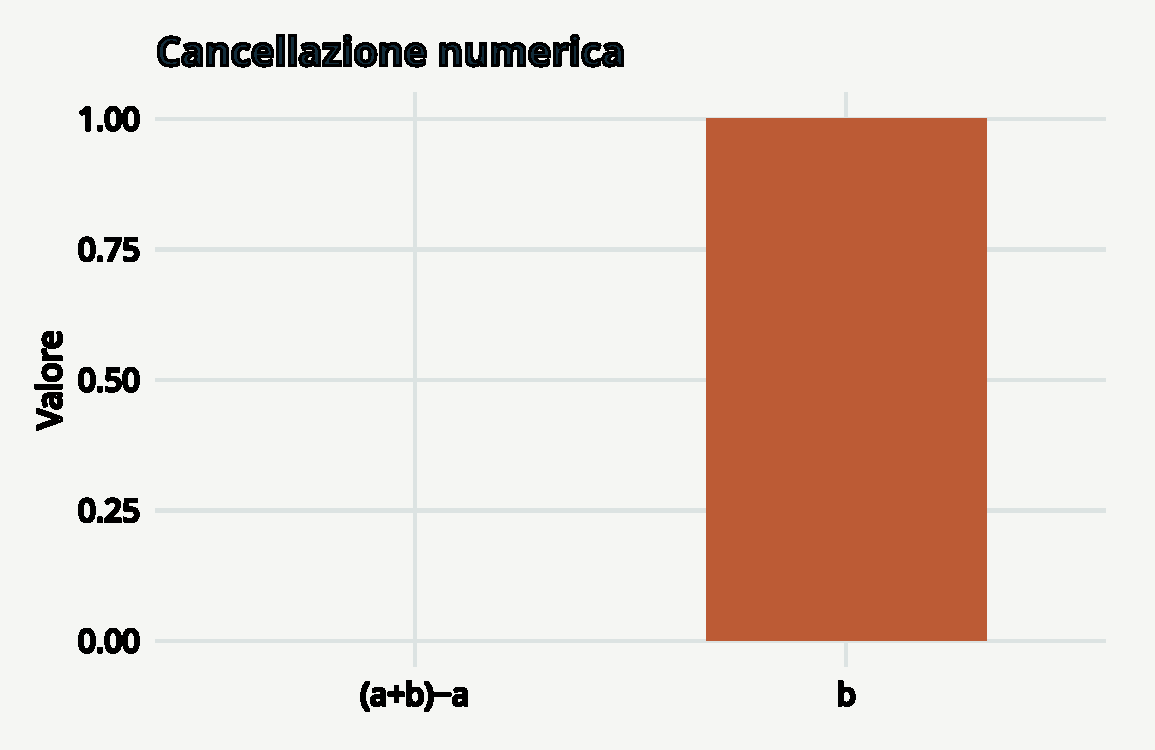
\includegraphics[width=\linewidth,height=6.0cm,keepaspectratio]{Esperimenti/t00-confronto-A.pdf}\par}
\PSmall{Esponente di a = 10\textasciicircum{}k: 16. Seme: 17.}
}};
\node[anchor=north west,inner sep=0] at([xshift=10.85cm,yshift=-2.12cm]current page.north west){\Colonna{8.16cm}{\PLabel{Scenario A · simulazione}
\PBody{Le due espressioni confrontate sono equivalenti nell’aritmetica esatta. Quando il valore di a diventa molto maggiore di b, la rappresentazione finita dei numeri può impedire che l’addizione conservi l’incremento più piccolo; la sottrazione successiva rende allora visibile l’informazione perduta.}
\par\smallskip{\centering\adjustbox{max width=.98\linewidth}{$\displaystyle (a+b)-a\quad\hbox{e}\quad b$}\par\smallskip}
\PSmall{$a=10^k$ è il valore di grande ampiezza; $b$ è l’incremento unitario; lo scarto assoluto confronta $(a+b)-a$ con $b$.}
}};
\node[anchor=north east,inner sep=0] at([xshift=17.1cm,yshift=-12.04cm]current page.north west){\fontsize{7.7}{9}\selectfont \href{https://marzione00.github.io/Lab_Geo/\#laboratorio/t00-confronto}{\color{Classical}\bfseries Apri il laboratorio · t00-confronto}};
\end{tikzpicture}\end{frame}

\begin{frame}[plain]\hypertarget{slide64}{}
\bookmark[level=1,page=64]{Confronto | Confrontare implementazioni}
\begin{tikzpicture}[remember picture,overlay]
\PilotChrome{Confronto | Confrontare implementazioni}{CONFRONTI E CONSEGNA DEL LAVORO}{64}{L’identità algebrica può produrre risultati numerici differenti in aritmetica finita.}
\node[anchor=north west,inner sep=0] at([xshift=.96cm,yshift=-2.12cm]current page.north west){\Colonna{9.40cm}{{\centering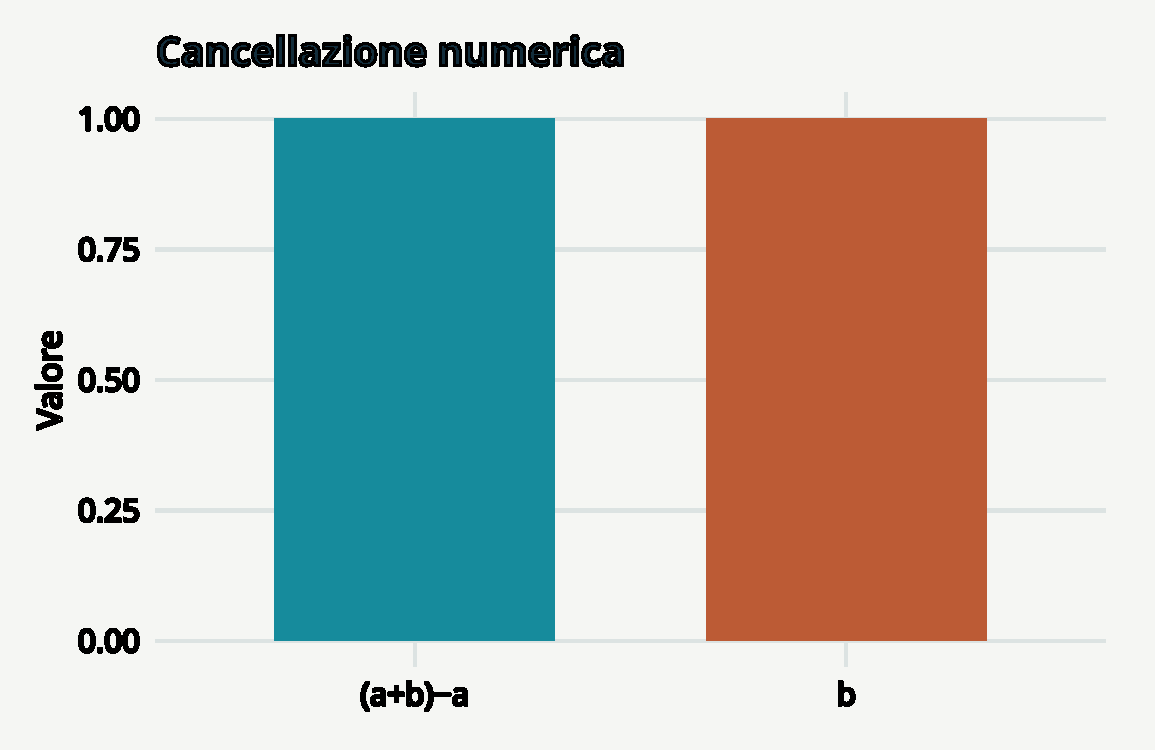
\includegraphics[width=\linewidth,height=5.6cm,keepaspectratio]{Esperimenti/t00-confronto-B.pdf}\par}
\PSmall{Esponente di a = 10\textasciicircum{}k: 16 $\to$ 10. Tutti gli altri parametri e il seme sono fissi.}
}};
\node[anchor=north west,inner sep=0] at([xshift=10.85cm,yshift=-2.12cm]current page.north west){\Colonna{8.16cm}{\PLabel{Confronto fra gli scenari}
{\fontsize{10.2}{12.8}\selectfont\begin{tabular}{@{}>{\raggedright\arraybackslash}p{0.48\linewidth}@{\hspace{.13cm}}>{\raggedright\arraybackslash}p{0.224\linewidth}@{\hspace{.13cm}}>{\raggedright\arraybackslash}p{0.224\linewidth}@{}}\toprule Grandezza & A & B\\[2.3pt]
\midrule 
Scarto assoluto & 1 & 0\\[2.3pt]
Entro tolleranza & 0 & 1\\[2.3pt]
\bottomrule\end{tabular}\par}
\vspace{.25cm}\PBody{A ordine di grandezza più piccolo il termine unitario si conserva nel calcolo. Lo scarto passa da uno a zero.}
}};
\node[anchor=north east,inner sep=0] at([xshift=17.1cm,yshift=-12.04cm]current page.north west){\fontsize{7.7}{9}\selectfont \href{https://marzione00.github.io/Lab_Geo/\#laboratorio/t00-confronto}{\color{Classical}\bfseries Apri il laboratorio · t00-confronto}};
\end{tikzpicture}\end{frame}

\begin{frame}[plain]\hypertarget{slide65}{}
\bookmark[level=1,page=65]{Dal risultato alla relazione}
\begin{tikzpicture}[remember picture,overlay]
\PilotChrome{Dal risultato alla relazione}{SINTESI}{65}{Conserva il file di ingresso e una procedura che ricalcoli il risultato in una sessione pulita.}
\node[anchor=north west,inner sep=0] at([xshift=.96cm,yshift=-2.12cm]current page.north west){\Colonna{9.40cm}{\PLabel{Domanda di partenza}
\PBody{Come si trasforma una misura in un risultato che un’altra persona può ricalcolare?}
\PLabel{Risultato da discutere}
\PBody{Per il primo provino, 107,2 g divisi per 40 cm³ danno 2,68 g/cm³. Due linguaggi possono riprodurre il rapporto quando unità, righe e regole sui mancanti coincidono.}
}};
\node[anchor=north west,inner sep=0] at([xshift=10.85cm,yshift=-2.12cm]current page.north west){\Colonna{8.16cm}{\PLabel{Limiti della conclusione}
\PBody{Tre provini aiutano a verificare il codice. Per descrivere un affioramento occorrono il disegno di prelievo e l’identità delle stazioni.}
\vspace{.4cm}\href{https://marzione00.github.io/Lab_Geo/\#modulo-M01}{\color{Classical}\bfseries Prosegui · M01 · Pensare con i dati}}};
\end{tikzpicture}\end{frame}

\begin{frame}[plain]\hypertarget{slide66}{}
\bookmark[level=1,page=66]{Fonti, dati e codice per riprodurre le figure}
\begin{tikzpicture}[remember picture,overlay]
\PilotChrome{Fonti, dati e codice per riprodurre le figure}{RIFERIMENTI}{66}{Per confrontare due implementazioni usa lo stesso input e la stessa convenzione numerica.}
\node[anchor=north west,inner sep=0] at([xshift=.96cm,yshift=-2.12cm]current page.north west){\Colonna{9.40cm}{\PLabel{Materiali del corso}
\PBody{Il fascicolo deriva dal modulo T00 di GeoStat Lab e dai materiali didattici di Marzio De Corato. I dati del caso guida sono didattici. Le simulazioni A e B riportano il proprio seme.}
\href{https://github.com/marzione00/Lab_Geo/blob/649f7cc577b96bd1044d81e78a2f530813e4f96b/moduli/T00/README.md}{\color{Classical}\bfseries Scheda e documentazione originale}\par\smallskip \href{https://github.com/marzione00/Lab_Geo/blob/649f7cc577b96bd1044d81e78a2f530813e4f96b/materiali/R/T00_figure.R}{\color{Classical}\bfseries Script R delle figure del corso}}};
\node[anchor=north west,inner sep=0] at([xshift=10.85cm,yshift=-2.12cm]current page.north west){\Colonna{8.16cm}{\PLabel{Nell’archivio dei sorgenti}
\PBody{Codice contiene i frammenti delle pagine. Esperimenti comprende i due programmi R e i risultati di ciascun confronto. Diagrammi contiene i disegni TikZ modificabili. Scena conserva il modello Blender della copertina.}
\vspace{.4cm}\href{https://marzione00.github.io/Lab_Geo/\#modulo-T00}{\color{Classical}\bfseries Apri Basalto su GeoStat Lab}}};
\end{tikzpicture}\end{frame}

\end{document}